% !TEX root = ./Praxisbericht.tex
% https://github.com/James-Yu/LaTeX-Workshop/wiki/Compile
% ------------------------------------------------------------
% LaTeX Template für die DHBW zum Schnellstart!
% Original: https://github.wdf.sap.corp/vtgermany/LaTeX-Template-DHBW
% ------------------------------------------------------------
% ---- Präambel mit Angaben zum Dokument
% !TEX root = ../../Praxisbericht.tex
\documentclass[
    fontsize=12pt,           % Leitlinien sprechen von Schriftgröße 12.
    paper=A4,
    twoside=false,
    listof=totoc,            % Tabellen- und Abbildungsverzeichnis ins Inhaltsverzeichnis
    bibliography=totoc,      % Literaturverzeichnis ins Inhaltsverzeichnis aufnehmen
    titlepage,               % Titlepage-Umgebung anstatt \maketitle
    headsepline,             % horizontale Linie unter Kolumnentitel
    abstract,                % Überschrift einschalten, Abstract muss in {abstract}-Umgebung stehen
    % final,                 % TODO:FINAL_COMPILATION Remove or change to final [final or draft]
]{scrreprt}                  % Verwendung von KOMA-Report
\pdfcompresslevel=0          % TODO:FINAL_COMPILATION Remove
\pdfobjcompresslevel=0       % TODO:FINAL_COMPILATION Remove

\usepackage[T1]{fontenc}     % Ausgabe von westeuropäischen Zeichen (auch Umlaute)
\usepackage{alphabeta}       % Griechische Buchstaben
\usepackage[utf8]{inputenc}  % UTF8 Encoding einschalten
\usepackage[ngerman]{babel}  % Neue deutsche Rechtschreibung
\usepackage{microtype}       % Trennung von Wörtern wird besser umgesetzt
\usepackage{lmodern}         % Nicht-gerasterte Schriftarten (bei MikTeX erforderlich)
\usepackage[draft]{graphicx} % Einbinden von Grafiken erlauben % TODO:FINAL_COMPILATION Remove or change to final [final or draft] single one can be viewed with \includegraphics[draft=false]{image.pdf}
\usepackage{wrapfig}         % Grafiken fließend im Text
\usepackage{setspace}        % Zeilenabstand \singlespacing, \onehalfspaceing, \doublespacing
\usepackage[
    %showframe,                % Ränder anzeigen lassen
    left=2.7cm, right=2.5cm,
    top=2.5cm,  bottom=2.5cm,
    includeheadfoot,
    showframe=true,             % TODO:FINAL_COMPILATION Remove
]{geometry}                      % Seitenlayout einstellen
\usepackage{scrlayer-scrpage}    % Gestaltung von Fuß- und Kopfzeilen
\KOMAoptions{draft=false}        % TODO:FINAL_COMPILATION Change to false
\usepackage{acronym}             % Abkürzungen, Abkürzungsverzeichnis
\usepackage{titletoc}            % Anpassungen am Inhaltsverzeichnis
\contentsmargin{0.75cm}          % Abstand im Inhaltsverzeichnis zw. Punkt und Seitenzahl
\usepackage[                     % Klickbare Links (enth. auch "nameref", "url" Package)
    hidelinks,                     % Blende die "URL Boxen" aus.
    breaklinks=true                % Breche zu lange URLs am Zeilenende um
]{hyperref}
\usepackage[hypcap=true, justification=centering]{caption}% Anker Anpassung für Referenzen
\urlstyle{same}                  % Aktuelle Schrift auch für URLs
% Anpassung von autoref für Gleichungen (ergänzt runde Klammern) und Algorithm.
% Anstatt "Listing" kann auch z.B. "Code-Ausschnitt" verwendet werden. Dies sollte
% jedoch synchron gehalten werden mit \lstlistingname (siehe weiter unten).
\addto\extrasngerman{%
    \def\equationautorefname~#1\null{Gleichung~(#1)\null}
    \def\lstnumberautorefname{Zeile}
    \def\lstlistingautorefname{Listing}
    \def\algorithmautorefname{Algorithmus}
    % Damit einheitlich "Abschnitt 1.2[.3]" verwendet wird und nicht "Unterabschnitt 1.2.3"
    % \def\subsectionautorefname{Abschnitt}
}

% ---- Abstand verkleinern von der Überschrift
\renewcommand*{\chapterheadstartvskip}{\vspace*{.5\baselineskip}}

% Hierdurch werden Schusterjungen und Hurenkinder vermieden, d.h. einzelne Wörter
% auf der nächsten Seite oder in einer einzigen Zeile.
% LaTeX kann diese dennoch erzeugen, falls das Layout ansonsten nicht umsetzbar ist.
% Diese Werte sind aber gute Startwerte.
\widowpenalty10000
\clubpenalty10000

% ---- Für das Quellenverzeichnis
\usepackage[
    backend = biber,                % Verweis auf biber
    language = auto,
    style = numeric,                % Nummerierung der Quellen mit Zahlen
    sorting = none,                 % none = Sortierung nach der Erscheinung im Dokument
    sortcites = true,               % Sortiert die Quellen innerhalb eines cite-Befehls
    block = space,                  % Extra Leerzeichen zwischen Blocks
    hyperref = true,                % Links sind klickbar auch in der Quelle
    %backref = true,                % Referenz, auf den Text an die zitierte Stelle
    bibencoding = auto,
    giveninits = true,              % Vornamen werden abgekürzt
    doi=false,                      % DOI nicht anzeigen
    isbn=false,                     % ISBN nicht anzeigen
    alldates=short                  % Datum immer als DD.MM.YYYY anzeigen
]{biblatex}
\addbibresource{Inhalt/literatur.bib}
\setcounter{biburlnumpenalty}{3000}     % Umbruchgrenze für Zahlen
\setcounter{biburlucpenalty}{6000}      % Umbruchgrenze für Großbuchstaben
\setcounter{biburllcpenalty}{9000}      % Umbruchgrenze für Kleinbuchstaben
\DeclareNameAlias{default}{family-given}  % Nachname vor dem Vornamen
\AtBeginBibliography{\renewcommand{\multinamedelim}{\addslash\space
    }\renewcommand{\finalnamedelim}{\multinamedelim}}  % Schrägstrich zwischen den Autorennamen
\DefineBibliographyStrings{german}{
    urlseen = {Einsichtnahme:},                      % Ändern des Titels von "besucht am"
}
\usepackage[babel,german=quotes]{csquotes}         % Deutsche Anführungszeichen + Zitate


% ---- Für Mathevorlage
\usepackage{amsmath}    % Erweiterung vom Mathe-Satz
\usepackage{amssymb}    % Lädt amsfonts und weitere Symbole
\usepackage{amsfonts}
\usepackage{MnSymbol}   % Für Symbole, die in amssymb nicht enthalten sind.
\usepackage{mathtools}
\usepackage{nccmath}
\usepackage{scrextend}
\setcounter{MaxMatrixCols}{40}

% ---- Für Quellcodevorlage
\usepackage{scrhack}                    % Hack zur Verw. von listings in KOMA-Script
\usepackage{listings}                   % Darstellung von Quellcode
\usepackage[table,xcdraw]{xcolor}       % Einfache Verwendung von Farben
% -- Eigene Farben für den Quellcode
\definecolor{JavaLila}{rgb}{0.4,0.1,0.4}
\definecolor{JavaGruen}{rgb}{0.3,0.5,0.4}
\definecolor{JavaBlau}{rgb}{0.0,0.0,1.0}
\definecolor{ABAPKeywordsBlue}{HTML}{6000ff}
\definecolor{ABAPCommentGrey}{HTML}{808080}
\definecolor{ABAPStringGreen}{HTML}{4da619}
\definecolor{PyKeywordsBlue}{HTML}{0000AC}
\definecolor{PyCommentGrey}{HTML}{808080}
\definecolor{PyStringGreen}{HTML}{008080}
% -- Farben für ABAP CDS
\definecolor{CDSString}{HTML}{FF8C00}
\definecolor{CDSKeywords}{HTML}{6000ff}
\definecolor{CDSAnnotation}{HTML}{00BFFF}
\definecolor{CDSComment}{HTML}{808080}
\definecolor{CDSFunc}{HTML}{FF0000}

% -- Default Listing-Styles

\lstset{
% Das Paket "listings" kann kein UTF-8. Deswegen werden hier
% die häufigsten Zeichen definiert (ä,ö,ü,...)
literate=%
    {á}{{\'a}}1 {é}{{\'e}}1 {í}{{\'i}}1 {ó}{{\'o}}1 {ú}{{\'u}}1
{Á}{{\'A}}1 {É}{{\'E}}1 {Í}{{\'I}}1 {Ó}{{\'O}}1 {Ú}{{\'U}}1
{à}{{\`a}}1 {è}{{\`e}}1 {ì}{{\`i}}1 {ò}{{\`o}}1 {ù}{{\`u}}1
{À}{{\`A}}1 {È}{{\'E}}1 {Ì}{{\`I}}1 {Ò}{{\`O}}1 {Ù}{{\`U}}1
{ä}{{\"a}}1 {ë}{{\"e}}1 {ï}{{\"i}}1 {ö}{{\"o}}1 {ü}{{\"u}}1
{Ä}{{\"A}}1 {Ë}{{\"E}}1 {Ï}{{\"I}}1 {Ö}{{\"O}}1 {Ü}{{\"U}}1
{â}{{\^a}}1 {ê}{{\^e}}1 {î}{{\^i}}1 {ô}{{\^o}}1 {û}{{\^u}}1
{Â}{{\^A}}1 {Ê}{{\^E}}1 {Î}{{\^I}}1 {Ô}{{\^O}}1 {Û}{{\^U}}1
{œ}{{\oe}}1 {Œ}{{\OE}}1 {æ}{{\ae}}1 {Æ}{{\AE}}1 {ß}{{\ss}}1
{ű}{{\H{u}}}1 {Ű}{{\H{U}}}1 {ő}{{\H{o}}}1 {Ő}{{\H{O}}}1
{ç}{{\c c}}1 {Ç}{{\c C}}1 {ø}{{\o}}1 {å}{{\r a}}1 {Å}{{\r A}}1
{€}{{\euro}}1 {£}{{\pounds}}1 {«}{{\guillemotleft}}1
{»}{{\guillemotright}}1 {ñ}{{\~n}}1 {Ñ}{{\~N}}1 {¿}{{?`}}1,
breaklines=true,        % Breche lange Zeilen um
breakatwhitespace=true, % Wenn möglich, bei Leerzeichen umbrechen
% Symbol für Zeilenumbruch einfügen
prebreak=\raisebox{0ex}[0ex][0ex]{\ensuremath{\rhookswarrow}},
postbreak=\raisebox{0ex}[0ex][0ex]{\ensuremath{\rcurvearrowse\space}},
tabsize=4,                                 % Setze die Breite eines Tabs
basicstyle=\ttfamily\small,                % Grundsätzlicher Schriftstyle
columns=fixed,                             % Besseres Schriftbild
numbers=left,                              % Nummerierung der Zeilen
%frame=single,                             % Umrandung des Codes
showstringspaces=false,                    % Keine Leerzeichen hervorheben
keywordstyle=\color{blue},
ndkeywordstyle=\bfseries\color{darkgray},
identifierstyle=\color{black},
commentstyle=\itshape\color{JavaGruen},   % Kommentare in eigener Farbe
stringstyle=\color{JavaBlau},             % Strings in eigener Farbe,
captionpos=b,                             % Bild*unter*schrift
xleftmargin=5.0ex
}

% ---- Eigener JAVA-Style für den Quellcode
\renewcommand{\ttdefault}{pcr}               % Schriftart, welche auch fett beinhaltet
\lstdefinestyle{EigenerJavaStyle}{
    language=Java,                             % Syntax Highlighting für Java
    %frame=single,                             % Umrandung des Codes
    keywordstyle=\bfseries\color{JavaLila},    % Keywords in eigener Farbe und fett
    commentstyle=\itshape\color{JavaGruen},    % Kommentare in eigener Farbe und italic
    stringstyle=\color{JavaBlau}               % Strings in eigener Farbe
}

% ---- Eigener ABAP-Style für den Quellcode
\renewcommand{\ttdefault}{pcr}
\lstdefinestyle{EigenerABAPStyle}{
    language=[R/3 6.10]ABAP,
    morestring=[b]\|,                          % Für Pipe-Strings
    morestring=[b]\`,                          % für Backtick-Strings
    keywordstyle=\bfseries\color{ABAPKeywordsBlue},
    commentstyle=\itshape\color{ABAPCommentGrey},
    stringstyle=\color{ABAPStringGreen},
    tabsize=2,
    morekeywords={
            types,
            @data,
            as,
            lower,
            start,
            selection,
            order,
            by,
            inner,
            join,
            key,
            end,
            cast,
            optional,
            returning,
            badi,
            default,
            standard,
            length,
            begin,
            filters,
            final,
            global,
            friends,
            interfaces,
            endclass,
            endinterface,
            interface,
            implementation,
            eq,
            lt,
            gt,
            index,
            reference,
            symbol,
            assigning
        }
}

% ---- Eigener Python-Style für den Quellcode
\renewcommand{\ttdefault}{pcr}
\lstdefinestyle{EigenerPythonStyle}{
    language=Python,
    columns=flexible,
    keywordstyle=\bfseries\color{PyKeywordsBlue},
    commentstyle=\itshape\color{PyCommentGrey},
    stringstyle=\color{PyStringGreen}
}

%----- ABAP-CDS-View language
\lstdefinelanguage{ABAPCDS}{
    sensitive=false,
    %Keywords
    morekeywords={define,
            view,
            as,
            select,
            from,
            inner,
            join,
            on,
            key,
            case,
            when,
            then,
            else,
            end,
            true,
            false,
            cast,
            where,
            and,
            distinct,
            group,
            by,
            having,
            min,
            sum,
            max,
            count,
            avg
        },
    %Methoden
    morekeywords=[2]{
            div,
            currency\_conversion,
            dats\_days\_between,
            concat\_with\_space,
            dats\_add_days,
            dats\_is\_valid,
            dats\_add\_months,
            unit\_conversion,
            division,
            mod,
            abs,
            floor,
            ceil,
            round,
            concat,
            replace,
            substring,
            left,
            right,
            length
        },
    morecomment=[s][\color{CDSAnnotation}]{@}{:},
    morecomment=[l][\itshape\color{CDSComment}]{//},
    morecomment=[s][\itshape\color{CDSComment}]{/*}{*/},
    morestring=[b][\color{CDSString}]',
    keywordstyle=\bfseries\color{CDSKeywords},
    keywordstyle=[2]\color{CDSFunc}
}

% ---- JavaScript
\lstdefinelanguage{JavaScript}{
    morekeywords=[1]{await, async, break, case, catch, class, const, constructor, continue, debugger, default, delete, do, else, enum, export, extends, finally, for, from, function, if, implements, import, in, instanceof, new, return, super, switch, this, throw, try, typeof, var, void, while, with, yield, get, set, static, of, let, throw, try},
    % Literals, primitive types, and reference types.
    morekeywords=[2]{false, null, true, boolean, number, undefined,
            Array, Boolean, Date, Math, Number, String, Object, NaN, Symbol},
    % Built-ins.
    morekeywords=[3]{eval, parseInt, parseFloat, escape, unescape},
    sensitive=true,
    morecomment=[s]{/*}{*/},
    morecomment=[l]//,
    morecomment=[s]{/**}{*/}, % JavaDoc style comments
    morestring=[b]',
    morestring=[b]",
    morestring=[b]` % Interpolation strings.
}

% ---- TypeScript
\renewcommand{\ttdefault}{pcr}
\lstdefinestyle{Typescript}{
    language=JavaScript,
    morekeywords={
            type,
            interface,
            as,
            implements,
            package,
            namespace,
            private,
            protected,
            public,
            any,
            unknown,
            declare,
            module,
            require,
            from,
            symbol,
            keyof,
            infer,
            abstract
        }
}


\lstdefinelanguage{Rust}{%
  sensitive%
, morecomment=[l]{//}%
, morecomment=[s]{/*}{*/}%
, moredelim=[s][{\itshape\color[rgb]{0,0,0.75}}]{\#[}{]}%
, morestring=[b]{"}%
, alsodigit={}%
, alsoother={}%
, alsoletter={!}%
%
%
% [1] reserve keywords
% [2] traits
% [3] primitive types
% [4] type and value constructors
% [5] identifier
%
, morekeywords={break, continue, else, for, if, in, loop, match, return, while}  % control flow keywords
, morekeywords={as, const, let, move, mut, ref, static}  % in the context of variables
, morekeywords={dyn, enum, fn, impl, Self, self, struct, trait, type, union, use, where}  % in the context of declarations
, morekeywords={crate, extern, mod, pub, super}  % in the context of modularisation
, morekeywords={unsafe}  % markers
, morekeywords={abstract, alignof, become, box, do, final, macro, offsetof, override, priv, proc, pure, sizeof, typeof, unsized, virtual, yield}  % reserved identifiers
%
% grep 'pub trait [A-Za-z][A-Za-z0-9]*' -r . | sed 's/^.*pub trait \([A-Za-z][A-Za-z0-9]*\).*/\1/g' | sort -u | tr '\n' ',' | sed 's/^\(.*\),$/{\1}\n/g' | sed 's/,/, /g'
, morekeywords=[2]{Add, AddAssign, Any, AsciiExt, AsInner, AsInnerMut, AsMut, AsRawFd, AsRawHandle, AsRawSocket, AsRef, Binary, BitAnd, BitAndAssign, Bitor, BitOr, BitOrAssign, BitXor, BitXorAssign, Borrow, BorrowMut, Boxed, BoxPlace, BufRead, BuildHasher, CastInto, CharExt, Clone, CoerceUnsized, CommandExt, Copy, Debug, DecodableFloat, Default, Deref, DerefMut, DirBuilderExt, DirEntryExt, Display, Div, DivAssign, DoubleEndedIterator, DoubleEndedSearcher, Drop, EnvKey, Eq, Error, ExactSizeIterator, ExitStatusExt, Extend, FileExt, FileTypeExt, Float, Fn, FnBox, FnMut, FnOnce, Freeze, From, FromInner, FromIterator, FromRawFd, FromRawHandle, FromRawSocket, FromStr, FullOps, FusedIterator, Generator, Hash, Hasher, Index, IndexMut, InPlace, Int, Into, IntoCow, IntoInner, IntoIterator, IntoRawFd, IntoRawHandle, IntoRawSocket, IsMinusOne, IsZero, Iterator, JoinHandleExt, LargeInt, LowerExp, LowerHex, MetadataExt, Mul, MulAssign, Neg, Not, Octal, OpenOptionsExt, Ord, OsStrExt, OsStringExt, Packet, PartialEq, PartialOrd, Pattern, PermissionsExt, Place, Placer, Pointer, Product, Put, RangeArgument, RawFloat, Read, Rem, RemAssign, Seek, Shl, ShlAssign, Shr, ShrAssign, Sized, SliceConcatExt, SliceExt, SliceIndex, Stats, Step, StrExt, Sub, SubAssign, Sum, Sync, TDynBenchFn, Terminal, Termination, ToOwned, ToSocketAddrs, ToString, Try, TryFrom, TryInto, UnicodeStr, Unsize, UpperExp, UpperHex, WideInt, Write}
, morekeywords=[2]{Send}  % additional traits
%
, morekeywords=[3]{bool, char, f32, f64, i8, i16, i32, i64, isize, str, u8, u16, u32, u64, unit, usize, i128, u128}  % primitive types
%
, morekeywords=[4]{Err, false, None, Ok, Some, true}  % prelude value constructors
% grep 'pub \(type\|struct\|enum\) [A-Za-z][A-Za-z0-9]*' -r . | sed 's/^.*pub \(type\|struct\|enum\) \([A-Za-z][A-Za-z0-9]*\).*/\2/g' | sort -u | tr '\n' ',' | sed 's/^\(.*\),$/{\1}\n/g' | sed 's/,/, /g'
, morekeywords=[3]{AccessError, Adddf3, AddI128, AddoI128, AddoU128, ADDRESS, ADDRESS64, addrinfo, ADDRINFOA, AddrParseError, Addsf3, AddU128, advice, aiocb, Alignment, AllocErr, AnonPipe, Answer, Arc, Args, ArgsInnerDebug, ArgsOs, Argument, Arguments, ArgumentV1, Ashldi3, Ashlti3, Ashrdi3, Ashrti3, AssertParamIsClone, AssertParamIsCopy, AssertParamIsEq, AssertUnwindSafe, AtomicBool, AtomicPtr, Attr, auxtype, auxv, BackPlace, BacktraceContext, Barrier, BarrierWaitResult, Bencher, BenchMode, BenchSamples, BinaryHeap, BinaryHeapPlace, blkcnt, blkcnt64, blksize, BOOL, boolean, BOOLEAN, BoolTrie, BorrowError, BorrowMutError, Bound, Box, bpf, BTreeMap, BTreeSet, Bucket, BucketState, Buf, BufReader, BufWriter, Builder, BuildHasherDefault, BY, BYTE, Bytes, CannotReallocInPlace, cc, Cell, Chain, CHAR, CharIndices, CharPredicateSearcher, Chars, CharSearcher, CharsError, CharSliceSearcher, CharTryFromError, Child, ChildPipes, ChildStderr, ChildStdin, ChildStdio, ChildStdout, Chunks, ChunksMut, ciovec, clock, clockid, Cloned, cmsgcred, cmsghdr, CodePoint, Color, ColorConfig, Command, CommandEnv, Component, Components, CONDITION, condvar, Condvar, CONSOLE, CONTEXT, Count, Cow, cpu, CRITICAL, CStr, CString, CStringArray, Cursor, Cycle, CycleIter, daddr, DebugList, DebugMap, DebugSet, DebugStruct, DebugTuple, Decimal, Decoded, DecodeUtf16, DecodeUtf16Error, DecodeUtf8, DefaultEnvKey, DefaultHasher, dev, device, Difference, Digit32, DIR, DirBuilder, dircookie, dirent, dirent64, DirEntry, Discriminant, DISPATCHER, Display, Divdf3, Divdi3, Divmoddi4, Divmodsi4, Divsf3, Divsi3, Divti3, dl, Dl, Dlmalloc, Dns, DnsAnswer, DnsQuery, dqblk, Drain, DrainFilter, Dtor, Duration, DwarfReader, DWORD, DWORDLONG, DynamicLibrary, Edge, EHAction, EHContext, Elf32, Elf64, Empty, EmptyBucket, EncodeUtf16, EncodeWide, Entry, EntryPlace, Enumerate, Env, epoll, errno, Error, ErrorKind, EscapeDebug, EscapeDefault, EscapeUnicode, event, Event, eventrwflags, eventtype, ExactChunks, ExactChunksMut, EXCEPTION, Excess, ExchangeHeapSingleton, exit, exitcode, ExitStatus, Failure, fd, fdflags, fdsflags, fdstat, ff, fflags, File, FILE, FileAttr, filedelta, FileDesc, FilePermissions, filesize, filestat, FILETIME, filetype, FileType, Filter, FilterMap, Fixdfdi, Fixdfsi, Fixdfti, Fixsfdi, Fixsfsi, Fixsfti, Fixunsdfdi, Fixunsdfsi, Fixunsdfti, Fixunssfdi, Fixunssfsi, Fixunssfti, Flag, FlatMap, Floatdidf, FLOATING, Floatsidf, Floatsisf, Floattidf, Floattisf, Floatundidf, Floatunsidf, Floatunsisf, Floatuntidf, Floatuntisf, flock, ForceResult, FormatSpec, Formatted, Formatter, Fp, FpCategory, fpos, fpos64, fpreg, fpregset, FPUControlWord, Frame, FromBytesWithNulError, FromUtf16Error, FromUtf8Error, FrontPlace, fsblkcnt, fsfilcnt, fsflags, fsid, fstore, fsword, FullBucket, FullBucketMut, FullDecoded, Fuse, GapThenFull, GeneratorState, gid, glob, glob64, GlobalDlmalloc, greg, group, GROUP, Guard, GUID, Handle, HANDLE, Handler, HashMap, HashSet, Heap, HINSTANCE, HMODULE, hostent, HRESULT, id, idtype, if, ifaddrs, IMAGEHLP, Immut, in, in6, Incoming, Infallible, Initializer, ino, ino64, inode, input, InsertResult, Inspect, Instant, int16, int32, int64, int8, integer, IntermediateBox, Internal, Intersection, intmax, IntoInnerError, IntoIter, IntoStringError, intptr, InvalidSequence, iovec, ip, IpAddr, ipc, Ipv4Addr, ipv6, Ipv6Addr, Ipv6MulticastScope, Iter, IterMut, itimerspec, itimerval, jail, JoinHandle, JoinPathsError, KDHELP64, kevent, kevent64, key, Key, Keys, KV, l4, LARGE, lastlog, launchpad, Layout, Lazy, lconv, Leaf, LeafOrInternal, Lines, LinesAny, LineWriter, linger, linkcount, LinkedList, load, locale, LocalKey, LocalKeyState, Location, lock, LockResult, loff, LONG, lookup, lookupflags, LookupHost, LPBOOL, LPBY, LPBYTE, LPCSTR, LPCVOID, LPCWSTR, LPDWORD, LPFILETIME, LPHANDLE, LPOVERLAPPED, LPPROCESS, LPPROGRESS, LPSECURITY, LPSTARTUPINFO, LPSTR, LPVOID, LPWCH, LPWIN32, LPWSADATA, LPWSAPROTOCOL, LPWSTR, Lshrdi3, Lshrti3, lwpid, M128A, mach, major, Map, mcontext, Metadata, Metric, MetricMap, mflags, minor, mmsghdr, Moddi3, mode, Modsi3, Modti3, MonitorMsg, MOUNT, mprot, mq, mqd, msflags, msghdr, msginfo, msglen, msgqnum, msqid, Muldf3, Mulodi4, Mulosi4, Muloti4, Mulsf3, Multi3, Mut, Mutex, MutexGuard, MyCollection, n16, NamePadding, NativeLibBoilerplate, nfds, nl, nlink, NodeRef, NoneError, NonNull, NonZero, nthreads, NulError, OccupiedEntry, off, off64, oflags, Once, OnceState, OpenOptions, Option, Options, OptRes, Ordering, OsStr, OsString, Output, OVERLAPPED, Owned, Packet, PanicInfo, Param, ParseBoolError, ParseCharError, ParseError, ParseFloatError, ParseIntError, ParseResult, Part, passwd, Path, PathBuf, PCONDITION, PCONSOLE, Peekable, PeekMut, Permissions, PhantomData, pid, Pipes, PlaceBack, PlaceFront, PLARGE, PoisonError, pollfd, PopResult, port, Position, Powidf2, Powisf2, Prefix, PrefixComponent, PrintFormat, proc, Process, PROCESS, processentry, protoent, PSRWLOCK, pthread, ptr, ptrdiff, PVECTORED, Queue, radvisory, RandomState, Range, RangeFrom, RangeFull, RangeInclusive, RangeMut, RangeTo, RangeToInclusive, RawBucket, RawFd, RawHandle, RawPthread, RawSocket, RawTable, RawVec, Rc, ReadDir, Receiver, recv, RecvError, RecvTimeoutError, ReentrantMutex, ReentrantMutexGuard, Ref, RefCell, RefMut, REPARSE, Repeat, Result, Rev, Reverse, riflags, rights, rlim, rlim64, rlimit, rlimit64, roflags, Root, RSplit, RSplitMut, RSplitN, RSplitNMut, RUNTIME, rusage, RwLock, RWLock, RwLockReadGuard, RwLockWriteGuard, sa, SafeHash, Scan, sched, scope, sdflags, SearchResult, SearchStep, SECURITY, SeekFrom, segment, Select, SelectionResult, sem, sembuf, send, Sender, SendError, servent, sf, Shared, shmatt, shmid, ShortReader, ShouldPanic, Shutdown, siflags, sigaction, SigAction, sigevent, sighandler, siginfo, Sign, signal, signalfd, SignalToken, sigset, sigval, Sink, SipHasher, SipHasher13, SipHasher24, size, SIZE, Skip, SkipWhile, Slice, SmallBoolTrie, sockaddr, SOCKADDR, sockcred, Socket, SOCKET, SocketAddr, SocketAddrV4, SocketAddrV6, socklen, speed, Splice, Split, SplitMut, SplitN, SplitNMut, SplitPaths, SplitWhitespace, spwd, SRWLOCK, ssize, stack, STACKFRAME64, StartResult, STARTUPINFO, stat, Stat, stat64, statfs, statfs64, StaticKey, statvfs, StatVfs, statvfs64, Stderr, StderrLock, StderrTerminal, Stdin, StdinLock, Stdio, StdioPipes, Stdout, StdoutLock, StdoutTerminal, StepBy, String, StripPrefixError, StrSearcher, subclockflags, Subdf3, SubI128, SuboI128, SuboU128, subrwflags, subscription, Subsf3, SubU128, Summary, suseconds, SYMBOL, SYMBOLIC, SymmetricDifference, SyncSender, sysinfo, System, SystemTime, SystemTimeError, Take, TakeWhile, tcb, tcflag, TcpListener, TcpStream, TempDir, TermInfo, TerminfoTerminal, termios, termios2, TestDesc, TestDescAndFn, TestEvent, TestFn, TestName, TestOpts, TestResult, Thread, threadattr, threadentry, ThreadId, tid, time, time64, timespec, TimeSpec, timestamp, timeval, timeval32, timezone, tm, tms, ToLowercase, ToUppercase, TraitObject, TryFromIntError, TryFromSliceError, TryIter, TryLockError, TryLockResult, TryRecvError, TrySendError, TypeId, U64x2, ucontext, ucred, Udivdi3, Udivmoddi4, Udivmodsi4, Udivmodti4, Udivsi3, Udivti3, UdpSocket, uid, UINT, uint16, uint32, uint64, uint8, uintmax, uintptr, ulflags, ULONG, ULONGLONG, Umoddi3, Umodsi3, Umodti3, UnicodeVersion, Union, Unique, UnixDatagram, UnixListener, UnixStream, Unpacked, UnsafeCell, UNWIND, UpgradeResult, useconds, user, userdata, USHORT, Utf16Encoder, Utf8Error, Utf8Lossy, Utf8LossyChunk, Utf8LossyChunksIter, utimbuf, utmp, utmpx, utsname, uuid, VacantEntry, Values, ValuesMut, VarError, Variables, Vars, VarsOs, Vec, VecDeque, vm, Void, WaitTimeoutResult, WaitToken, wchar, WCHAR, Weak, whence, WIN32, WinConsole, Windows, WindowsEnvKey, winsize, WORD, Wrapping, wrlen, WSADATA, WSAPROTOCOL, WSAPROTOCOLCHAIN, Wtf8, Wtf8Buf, Wtf8CodePoints, xsw, xucred, Zip, zx}
%
, morekeywords=[5]{assert!, assert_eq!, assert_ne!, cfg!, column!, compile_error!, concat!, concat_idents!, debug_assert!, debug_assert_eq!, debug_assert_ne!, env!, eprint!, eprintln!, file!, format!, format_args!, include!, include_bytes!, include_str!, line!, module_path!, option_env!, panic!, print!, println!, select!, stringify!, thread_local!, try!, unimplemented!, unreachable!, vec!, write!, writeln!}  % prelude macros
}%

\lstdefinestyle{colouredRust}%
{ basicstyle=\ttfamily%
, identifierstyle=%
, commentstyle=\color[gray]{0.4}%
, stringstyle=\color[rgb]{0, 0, 0.5}%
, keywordstyle=\bfseries% reserved keywords
, keywordstyle=[2]\color[rgb]{0.75, 0, 0}% traits
, keywordstyle=[3]\color[rgb]{0, 0.5, 0}% primitive types
, keywordstyle=[4]\color[rgb]{0, 0.5, 0}% type and value constructors
, keywordstyle=[5]\color[rgb]{0, 0, 0.75}% macros
, columns=spaceflexible%
, keepspaces=true%
, showspaces=false%
, showtabs=false%
, showstringspaces=true%
}%

\lstdefinestyle{boxed}{
  style=colouredRust%
, numbers=left%
, firstnumber=auto%
, numberblanklines=true%
, frame=trbL%
, numberstyle=\tiny%
, frame=leftline%
, numbersep=7pt%
, framesep=5pt%
, framerule=10pt%
, xleftmargin=15pt%
, backgroundcolor=\color[gray]{0.97}%
, rulecolor=\color[gray]{0.90}%
}  % Weitere Details sind ausgelagert

\usepackage{algorithm}                  % Für Algorithmen-Umgebung (ähnlich wie lstlistings Umgebung)
\usepackage{algpseudocode}              % Für Pseudocode. Füge "[noend]" hinzu, wenn du kein "endif",
% etc. haben willst.

\makeatletter                           % Sorgt dafür, dass man @ in Namen verwenden kann.
% Ansonsten gibt es in der nächsten Zeile einen Compilefehler.
\renewcommand{\ALG@name}{Algorithmus}   % Umbenennen von "Algorithm" im Header der Listings.
\makeatother                            % Zeichen wieder zurücksetzen
\renewcommand{\lstlistingname}{Codeausschnitt} % Erlaubt das Umbenennen von "Listing" in anderen Titel.

% ---- Tabellen
\usepackage{booktabs}  % Für schönere Tabellen. Enthält neue Befehle wie \midrule
\usepackage{multirow}  % Mehrzeilige Tabellen
\usepackage{siunitx}   % Für SI Einheiten und das Ausrichten Nachkommastellen
\sisetup{locale=DE, range-phrase={~bis~}, output-decimal-marker={,}} % Damit ein Komma und kein Punkt verwendet wird.
\usepackage{xfrac} % Für siunitx Option "fraction-function=\sfrac"

% ---- Für Definitionsboxen in der Einleitung
\usepackage{amsthm}                     % Liefert die Grundlagen für Theoreme
\usepackage[framemethod=tikz]{mdframed} % Boxen für die Umrandung
% ---- Definition für Highlight Boxen

% ---- Grundsätzliche Definition zum Style
\newtheoremstyle{defi}
{\topsep}         % Abstand oben
{\topsep}         % Abstand unten
{\normalfont}     % Schrift des Bodys
{0pt}             % Einschub der ersten Zeile
{\bfseries}       % Darstellung von der Schrift in der Überschrift
{:}               % Trennzeichen zwischen Überschrift und Body
{.5em}            % Abstand nach dem Trennzeichen zum Body Text
{\thmname{#3}}    % Name in eckigen Klammern
\theoremstyle{defi}

% ------ Definition zum Strich vor eines Texts
\newmdtheoremenv[
    hidealllines = true,       % Rahmen komplett ausblenden
    leftline = true,           % Linie links einschalten
    innertopmargin = 0pt,      % Abstand oben
    innerbottommargin = 4pt,   % Abstand unten
    innerrightmargin = 0pt,    % Abstand rechts
    linewidth = 3pt,           % Linienbreite
    linecolor = gray!40,       % Linienfarbe
]{defStrich}{Definition}     % Name der des formats "defStrich"

% ------ Definition zum Eck-Kasten um einen Text
\newmdtheoremenv[
    hidealllines = true,
    innertopmargin = 6pt,
    linecolor = gray!40,
    singleextra={              % Eck-Markierungen für die Definition
            \draw[line width=3pt,gray!50,line cap=rect] (O|-P) -- +(1cm,0pt);
            \draw[line width=3pt,gray!50,line cap=rect] (O|-P) -- +(0pt,-1cm);
            \draw[line width=3pt,gray!50,line cap=rect] (O-|P) -- +(-1cm,0pt);
            \draw[line width=3pt,gray!50,line cap=rect] (O-|P) -- +(0pt,1cm);
        }
]{defEckKasten}{Definition}  % Name der des formats "defEckKasten"  % Weitere Details sind ausgelagert

% ---- Für Todo Notes
\usepackage{todonotes}
\setlength {\marginparwidth }{2cm}      % Abstand für Todo Notizen

% ====================================================== OWN ====================================================== %
% =========================== LIBRARIES =========================== %
\usepackage{tikz}
\usetikzlibrary{shadows,calc}
\usetikzlibrary{shapes.misc, positioning}
\usetikzlibrary{ext.paths.ortho}
\usepackage[T1]{fontenc}% http://ctan.org/pkg/fontenc
\usepackage[export]{adjustbox}
\usepackage{makecell}
\usepackage{comment}
\usepackage{enumitem}
\usepackage{array}
\usepackage{xpatch}
\usepackage{longtable}

% =========================== GENERAL COMMANDS =========================== %
\newcommand{\tikzcircle}[1][red,fill=red]{\tikz[baseline=-0.5ex]\draw[#1,radius=4.5pt] (0,0) circle ;}%

% =========================== RIGHT CAPTION FORMAT =========================== %
% right format for captions. Number with dot (1.) inside table of contents, no dot (1) inside text

% for figures/images (adapted from https://tex.stackexchange.com/questions/27250/remove-dot-after-number-in-figure-captions-while-keeping-the-dot-in-chapter-sect)
\renewcommand*{\figureformat}{%
    \figurename~\thefigure%
    %  \autodot% DELETED
}

% for tables
\renewcommand*{\tableformat}{%
    \tablename~\thetable%
    %  \autodot% DELETED
}

% \renewcommand*{\lstlistingformat}{%
%     \lstlistingname~\thelstlisting
% }
% for code (adapted from https://tex.stackexchange.com/questions/597350/add-dot-after-number-of-listing-in-list-of-listings)
% BUG: does not work
\makeatletter
\xpatchcmd\lst@MakeCaption{\protect\numberline{\thelstlisting}\lst@@caption}{\protect\numberline{\thelstlisting.}\lst@@caption}{}{}
\makeatother

% =========================== FIGURES/IMAGES =========================== %
%  How to add a shadow under a picture: https://latex.org/forum/viewtopic.php?t=18644
% code adapted from https://tex.stackexchange.com/a/11483/3954

% some parameters for customization
\def\shadowshift{1pt,-1pt}
\def\shadowradius{8pt}

\colorlet{innercolor}{black!15}
\colorlet{outercolor}{gray!00}

% this draws a shadow under a rectangle node
\newcommand\drawshadow[1]{
    \begin{pgfonlayer}{shadow}
        \shade[outercolor,inner color=innercolor,outer color=outercolor] ($(#1.south west)+(\shadowshift)+(\shadowradius/2,\shadowradius/2)$) circle (\shadowradius);
        \shade[outercolor,inner color=innercolor,outer color=outercolor] ($(#1.north west)+(\shadowshift)+(\shadowradius/2,-\shadowradius/2)$) circle (\shadowradius);
        \shade[outercolor,inner color=innercolor,outer color=outercolor] ($(#1.south east)+(\shadowshift)+(-\shadowradius/2,\shadowradius/2)$) circle (\shadowradius);
        \shade[outercolor,inner color=innercolor,outer color=outercolor] ($(#1.north east)+(\shadowshift)+(-\shadowradius/2,-\shadowradius/2)$) circle (\shadowradius);
        \shade[top color=innercolor,bottom color=outercolor] ($(#1.south west)+(\shadowshift)+(\shadowradius/2,-\shadowradius/2)$) rectangle ($(#1.south east)+(\shadowshift)+(-\shadowradius/2,\shadowradius/2)$);
        \shade[left color=innercolor,right color=outercolor] ($(#1.south east)+(\shadowshift)+(-\shadowradius/2,\shadowradius/2)$) rectangle ($(#1.north east)+(\shadowshift)+(\shadowradius/2,-\shadowradius/2)$);
        \shade[bottom color=innercolor,top color=outercolor] ($(#1.north west)+(\shadowshift)+(\shadowradius/2,-\shadowradius/2)$) rectangle ($(#1.north east)+(\shadowshift)+(-\shadowradius/2,\shadowradius/2)$);
        \shade[outercolor,right color=innercolor,left color=outercolor] ($(#1.south west)+(\shadowshift)+(-\shadowradius/2,\shadowradius/2)$) rectangle ($(#1.north west)+(\shadowshift)+(\shadowradius/2,-\shadowradius/2)$);
        \filldraw ($(#1.south west)+(\shadowshift)+(\shadowradius/2,\shadowradius/2)$) rectangle ($(#1.north east)+(\shadowshift)-(\shadowradius/2,\shadowradius/2)$);
    \end{pgfonlayer}
}

% create a shadow layer, so that we don't need to worry about overdrawing other things
\pgfdeclarelayer{shadow}
\pgfsetlayers{shadow,main}

\newcommand\shadowimage[2][]{%
    \begin{figure}[!h]
        \centering
        \begin{tikzpicture}
            \centering
            \node[anchor=south west,inner sep=0] (image) at (0,0) {\includegraphics[#1]{#2}};
            \drawshadow{image}
        \end{tikzpicture}
    \end{figure}}

% =========================== TABLES =========================== %
% new column types for multiline + text justify + fixed width
\newcolumntype{L}[1]{>{\raggedright\let\newline\\\arraybackslash\hspace{0pt}}m{#1}}
\newcolumntype{C}[1]{>{\centering\let\newline\\\arraybackslash\hspace{0pt}}m{#1}}
\newcolumntype{R}[1]{>{\raggedleft\let\newline\\\arraybackslash\hspace{0pt}}m{#1}}

% =========================== ITEMIZE/ENUMERATION =========================== %
% item range e.g. 1.-5.
\def\itemrange#1{%
    \addtocounter{enumi}{1}%
    \edef\labelenumi{\theenumi.--\noexpand\theenumi.}%
    \addtocounter{enumi}{-1}%
    \addtocounter{enumi}{#1}%
    \item
    \def\labelenumi{\theenumi.}}

% =========================== ALGORITHM =========================== %
% full line comment
\algnewcommand{\LineComment}[1]{\State \(\triangleright\) #1}

% =========================== TIKZ IMAGES/ICONS =========================== %
\definecolor{colorPositive}{HTML}{30914c}
\definecolor{colorNeutral}{HTML}{e76500}
\definecolor{colorNegative}{HTML}{f53232}

\newcommand\positiveEvaluation{%
    \begin{tikzpicture}[baseline=-0.5ex]
        \coordinate  (a) at (-0.09,-0.02) {};
        \coordinate  (b) at (-0.04,-0.07) {};
        \coordinate  (c) at (0.08,0.04) {};
        \draw[colorPositive,fill=colorPositive,radius=4.5pt] (0,0) circle ;
        \draw[white, line width=0.35mm, line cap=round] (a.center) -- (b.center);
        \draw[white, line width=0.35mm, line cap=round] (b.center) -- (c.center);
    \end{tikzpicture}\hspace{0.25cm}}

\newcommand\neutralEvaluation{%
    \begin{tikzpicture}[baseline=-0.5ex]
        \draw[colorNeutral,fill=colorNeutral,radius=4.5pt] (0,0) circle ;
        % \draw[white,fill=white,radius=0.2mm] (0.075,0.05) circle ;
        % \draw[white,fill=white,radius=0.2mm] (-0.075,0.05) circle ;
        % \draw[rounded corners, white, line width=0.4mm] (-0.15,-0.05) -- (0.15,-0.05) -- cycle;
    \end{tikzpicture}\hspace{0.25cm}}

\newcommand\negativeEvaluation{%
    \begin{tikzpicture}[baseline=-0.5ex]
        \draw[colorNegative,fill=colorNegative,radius=4.5pt] (0,0) circle ;
        \draw[rounded corners, white, line width=0.4mm] (-0.115,0.115) -- (0.115,-0.115) -- cycle;
        \draw[rounded corners, white, line width=0.4mm] (-0.115,-0.115) -- (0.115,0.115) -- cycle;
    \end{tikzpicture}\hspace{0.25cm}}

% =========================== JUPYTER NOTEBOOK =========================== %
\newenvironment{defaultFontSize}
{
    \fontsize{10.95pt}{13.6pt}\selectfont
    % \fontsize{4pt}{4.5pt}\selectfont
}
{
    \fontsize{12}{14.5}\selectfont
}

\AtBeginDocument{%
    \def\PYZsq{\textquotesingle}% Upright quotes in Pygmentized code
}
\usepackage{upquote} % Upright quotes for verbatim code
\usepackage[breakable]{tcolorbox}
\usepackage{fancyvrb} % verbatim replacement that allows latex
\DefineVerbatimEnvironment{Highlighting}{Verbatim}{commandchars=\\\{\}}

\makeatletter
\def\PY@reset{\let\PY@it=\relax \let\PY@bf=\relax%
    \let\PY@ul=\relax \let\PY@tc=\relax%
    \let\PY@bc=\relax \let\PY@ff=\relax}
\def\PY@tok#1{\csname PY@tok@#1\endcsname}
\def\PY@toks#1+{\ifx\relax#1\empty\else%
    \PY@tok{#1}\expandafter\PY@toks\fi}
\def\PY@do#1{\PY@bc{\PY@tc{\PY@ul{%
    \PY@it{\PY@bf{\PY@ff{#1}}}}}}}
\def\PY#1#2{\PY@reset\PY@toks#1+\relax+\PY@do{#2}}

\@namedef{PY@tok@w}{\def\PY@tc##1{\textcolor[rgb]{0.73,0.73,0.73}{##1}}}
\@namedef{PY@tok@c}{\let\PY@it=\textit\def\PY@tc##1{\textcolor[rgb]{0.24,0.48,0.48}{##1}}}
\@namedef{PY@tok@cp}{\def\PY@tc##1{\textcolor[rgb]{0.61,0.40,0.00}{##1}}}
\@namedef{PY@tok@k}{\let\PY@bf=\textbf\def\PY@tc##1{\textcolor[rgb]{0.00,0.50,0.00}{##1}}}
\@namedef{PY@tok@kp}{\def\PY@tc##1{\textcolor[rgb]{0.00,0.50,0.00}{##1}}}
\@namedef{PY@tok@kt}{\def\PY@tc##1{\textcolor[rgb]{0.69,0.00,0.25}{##1}}}
\@namedef{PY@tok@o}{\def\PY@tc##1{\textcolor[rgb]{0.40,0.40,0.40}{##1}}}
\@namedef{PY@tok@ow}{\let\PY@bf=\textbf\def\PY@tc##1{\textcolor[rgb]{0.67,0.13,1.00}{##1}}}
\@namedef{PY@tok@nb}{\def\PY@tc##1{\textcolor[rgb]{0.00,0.50,0.00}{##1}}}
\@namedef{PY@tok@nf}{\def\PY@tc##1{\textcolor[rgb]{0.00,0.00,1.00}{##1}}}
\@namedef{PY@tok@nc}{\let\PY@bf=\textbf\def\PY@tc##1{\textcolor[rgb]{0.00,0.00,1.00}{##1}}}
\@namedef{PY@tok@nn}{\let\PY@bf=\textbf\def\PY@tc##1{\textcolor[rgb]{0.00,0.00,1.00}{##1}}}
\@namedef{PY@tok@ne}{\let\PY@bf=\textbf\def\PY@tc##1{\textcolor[rgb]{0.80,0.25,0.22}{##1}}}
\@namedef{PY@tok@nv}{\def\PY@tc##1{\textcolor[rgb]{0.10,0.09,0.49}{##1}}}
\@namedef{PY@tok@no}{\def\PY@tc##1{\textcolor[rgb]{0.53,0.00,0.00}{##1}}}
\@namedef{PY@tok@nl}{\def\PY@tc##1{\textcolor[rgb]{0.46,0.46,0.00}{##1}}}
\@namedef{PY@tok@ni}{\let\PY@bf=\textbf\def\PY@tc##1{\textcolor[rgb]{0.44,0.44,0.44}{##1}}}
\@namedef{PY@tok@na}{\def\PY@tc##1{\textcolor[rgb]{0.41,0.47,0.13}{##1}}}
\@namedef{PY@tok@nt}{\let\PY@bf=\textbf\def\PY@tc##1{\textcolor[rgb]{0.00,0.50,0.00}{##1}}}
\@namedef{PY@tok@nd}{\def\PY@tc##1{\textcolor[rgb]{0.67,0.13,1.00}{##1}}}
\@namedef{PY@tok@s}{\def\PY@tc##1{\textcolor[rgb]{0.73,0.13,0.13}{##1}}}
\@namedef{PY@tok@sd}{\let\PY@it=\textit\def\PY@tc##1{\textcolor[rgb]{0.73,0.13,0.13}{##1}}}
\@namedef{PY@tok@si}{\let\PY@bf=\textbf\def\PY@tc##1{\textcolor[rgb]{0.64,0.35,0.47}{##1}}}
\@namedef{PY@tok@se}{\let\PY@bf=\textbf\def\PY@tc##1{\textcolor[rgb]{0.67,0.36,0.12}{##1}}}
\@namedef{PY@tok@sr}{\def\PY@tc##1{\textcolor[rgb]{0.64,0.35,0.47}{##1}}}
\@namedef{PY@tok@ss}{\def\PY@tc##1{\textcolor[rgb]{0.10,0.09,0.49}{##1}}}
\@namedef{PY@tok@sx}{\def\PY@tc##1{\textcolor[rgb]{0.00,0.50,0.00}{##1}}}
\@namedef{PY@tok@m}{\def\PY@tc##1{\textcolor[rgb]{0.40,0.40,0.40}{##1}}}
\@namedef{PY@tok@gh}{\let\PY@bf=\textbf\def\PY@tc##1{\textcolor[rgb]{0.00,0.00,0.50}{##1}}}
\@namedef{PY@tok@gu}{\let\PY@bf=\textbf\def\PY@tc##1{\textcolor[rgb]{0.50,0.00,0.50}{##1}}}
\@namedef{PY@tok@gd}{\def\PY@tc##1{\textcolor[rgb]{0.63,0.00,0.00}{##1}}}
\@namedef{PY@tok@gi}{\def\PY@tc##1{\textcolor[rgb]{0.00,0.52,0.00}{##1}}}
\@namedef{PY@tok@gr}{\def\PY@tc##1{\textcolor[rgb]{0.89,0.00,0.00}{##1}}}
\@namedef{PY@tok@ge}{\let\PY@it=\textit}
\@namedef{PY@tok@gs}{\let\PY@bf=\textbf}
\@namedef{PY@tok@ges}{\let\PY@bf=\textbf\let\PY@it=\textit}
\@namedef{PY@tok@gp}{\let\PY@bf=\textbf\def\PY@tc##1{\textcolor[rgb]{0.00,0.00,0.50}{##1}}}
\@namedef{PY@tok@go}{\def\PY@tc##1{\textcolor[rgb]{0.44,0.44,0.44}{##1}}}
\@namedef{PY@tok@gt}{\def\PY@tc##1{\textcolor[rgb]{0.00,0.27,0.87}{##1}}}
\@namedef{PY@tok@err}{\def\PY@bc##1{{\setlength{\fboxsep}{\string -\fboxrule}\fcolorbox[rgb]{1.00,0.00,0.00}{1,1,1}{\strut ##1}}}}
\@namedef{PY@tok@kc}{\let\PY@bf=\textbf\def\PY@tc##1{\textcolor[rgb]{0.00,0.50,0.00}{##1}}}
\@namedef{PY@tok@kd}{\let\PY@bf=\textbf\def\PY@tc##1{\textcolor[rgb]{0.00,0.50,0.00}{##1}}}
\@namedef{PY@tok@kn}{\let\PY@bf=\textbf\def\PY@tc##1{\textcolor[rgb]{0.00,0.50,0.00}{##1}}}
\@namedef{PY@tok@kr}{\let\PY@bf=\textbf\def\PY@tc##1{\textcolor[rgb]{0.00,0.50,0.00}{##1}}}
\@namedef{PY@tok@bp}{\def\PY@tc##1{\textcolor[rgb]{0.00,0.50,0.00}{##1}}}
\@namedef{PY@tok@fm}{\def\PY@tc##1{\textcolor[rgb]{0.00,0.00,1.00}{##1}}}
\@namedef{PY@tok@vc}{\def\PY@tc##1{\textcolor[rgb]{0.10,0.09,0.49}{##1}}}
\@namedef{PY@tok@vg}{\def\PY@tc##1{\textcolor[rgb]{0.10,0.09,0.49}{##1}}}
\@namedef{PY@tok@vi}{\def\PY@tc##1{\textcolor[rgb]{0.10,0.09,0.49}{##1}}}
\@namedef{PY@tok@vm}{\def\PY@tc##1{\textcolor[rgb]{0.10,0.09,0.49}{##1}}}
\@namedef{PY@tok@sa}{\def\PY@tc##1{\textcolor[rgb]{0.73,0.13,0.13}{##1}}}
\@namedef{PY@tok@sb}{\def\PY@tc##1{\textcolor[rgb]{0.73,0.13,0.13}{##1}}}
\@namedef{PY@tok@sc}{\def\PY@tc##1{\textcolor[rgb]{0.73,0.13,0.13}{##1}}}
\@namedef{PY@tok@dl}{\def\PY@tc##1{\textcolor[rgb]{0.73,0.13,0.13}{##1}}}
\@namedef{PY@tok@s2}{\def\PY@tc##1{\textcolor[rgb]{0.73,0.13,0.13}{##1}}}
\@namedef{PY@tok@sh}{\def\PY@tc##1{\textcolor[rgb]{0.73,0.13,0.13}{##1}}}
\@namedef{PY@tok@s1}{\def\PY@tc##1{\textcolor[rgb]{0.73,0.13,0.13}{##1}}}
\@namedef{PY@tok@mb}{\def\PY@tc##1{\textcolor[rgb]{0.40,0.40,0.40}{##1}}}
\@namedef{PY@tok@mf}{\def\PY@tc##1{\textcolor[rgb]{0.40,0.40,0.40}{##1}}}
\@namedef{PY@tok@mh}{\def\PY@tc##1{\textcolor[rgb]{0.40,0.40,0.40}{##1}}}
\@namedef{PY@tok@mi}{\def\PY@tc##1{\textcolor[rgb]{0.40,0.40,0.40}{##1}}}
\@namedef{PY@tok@il}{\def\PY@tc##1{\textcolor[rgb]{0.40,0.40,0.40}{##1}}}
\@namedef{PY@tok@mo}{\def\PY@tc##1{\textcolor[rgb]{0.40,0.40,0.40}{##1}}}
\@namedef{PY@tok@ch}{\let\PY@it=\textit\def\PY@tc##1{\textcolor[rgb]{0.24,0.48,0.48}{##1}}}
\@namedef{PY@tok@cm}{\let\PY@it=\textit\def\PY@tc##1{\textcolor[rgb]{0.24,0.48,0.48}{##1}}}
\@namedef{PY@tok@cpf}{\let\PY@it=\textit\def\PY@tc##1{\textcolor[rgb]{0.24,0.48,0.48}{##1}}}
\@namedef{PY@tok@c1}{\let\PY@it=\textit\def\PY@tc##1{\textcolor[rgb]{0.24,0.48,0.48}{##1}}}
\@namedef{PY@tok@cs}{\let\PY@it=\textit\def\PY@tc##1{\textcolor[rgb]{0.24,0.48,0.48}{##1}}}

\def\PYZbs{\char`\\}
\def\PYZus{\char`\_}
\def\PYZob{\char`\{}
\def\PYZcb{\char`\}}
\def\PYZca{\char`\^}
\def\PYZam{\char`\&}
\def\PYZlt{\char`\<}
\def\PYZgt{\char`\>}
\def\PYZsh{\char`\#}
\def\PYZpc{\char`\%}
\def\PYZdl{\char`\$}
\def\PYZhy{\char`\-}
\def\PYZsq{\char`\'}
\def\PYZdq{\char`\"}
\def\PYZti{\char`\~}
% for compatibility with earlier versions
\def\PYZat{@}
\def\PYZlb{[}
\def\PYZrb{]}
\makeatother

\makeatletter
    \newbox\Wrappedcontinuationbox
    \newbox\Wrappedvisiblespacebox
    \newcommand*\Wrappedvisiblespace {\textcolor{red}{\textvisiblespace}}
    \newcommand*\Wrappedcontinuationsymbol {\textcolor{red}{\llap{\tiny$\m@th\hookrightarrow$}}}
    \newcommand*\Wrappedcontinuationindent {3ex }
    \newcommand*\Wrappedafterbreak {\kern\Wrappedcontinuationindent\copy\Wrappedcontinuationbox}
    % Take advantage of the already applied Pygments mark-up to insert
    % potential linebreaks for TeX processing.
    %        {, <, #, %, $, ' and ": go to next line.
    %        _, }, ^, &, >, - and ~: stay at end of broken line.
    % Use of \textquotesingle for straight quote.
    \newcommand*\Wrappedbreaksatspecials {%
        \def\PYGZus{\discretionary{\char`\_}{\Wrappedafterbreak}{\char`\_}}%
        \def\PYGZob{\discretionary{}{\Wrappedafterbreak\char`\{}{\char`\{}}%
        \def\PYGZcb{\discretionary{\char`\}}{\Wrappedafterbreak}{\char`\}}}%
        \def\PYGZca{\discretionary{\char`\^}{\Wrappedafterbreak}{\char`\^}}%
        \def\PYGZam{\discretionary{\char`\&}{\Wrappedafterbreak}{\char`\&}}%
        \def\PYGZlt{\discretionary{}{\Wrappedafterbreak\char`\<}{\char`\<}}%
        \def\PYGZgt{\discretionary{\char`\>}{\Wrappedafterbreak}{\char`\>}}%
        \def\PYGZsh{\discretionary{}{\Wrappedafterbreak\char`\#}{\char`\#}}%
        \def\PYGZpc{\discretionary{}{\Wrappedafterbreak\char`\%}{\char`\%}}%
        \def\PYGZdl{\discretionary{}{\Wrappedafterbreak\char`\$}{\char`\$}}%
        \def\PYGZhy{\discretionary{\char`\-}{\Wrappedafterbreak}{\char`\-}}%
        \def\PYGZsq{\discretionary{}{\Wrappedafterbreak\textquotesingle}{\textquotesingle}}%
        \def\PYGZdq{\discretionary{}{\Wrappedafterbreak\char`\"}{\char`\"}}%
        \def\PYGZti{\discretionary{\char`\~}{\Wrappedafterbreak}{\char`\~}}%
    }
    % Some characters . , ; ? ! / are not pygmentized.
    % This macro makes them "active" and they will insert potential linebreaks
    \newcommand*\Wrappedbreaksatpunct {%
        \lccode`\~`\.\lowercase{\def~}{\discretionary{\hbox{\char`\.}}{\Wrappedafterbreak}{\hbox{\char`\.}}}%
        \lccode`\~`\,\lowercase{\def~}{\discretionary{\hbox{\char`\,}}{\Wrappedafterbreak}{\hbox{\char`\,}}}%
        \lccode`\~`\;\lowercase{\def~}{\discretionary{\hbox{\char`\;}}{\Wrappedafterbreak}{\hbox{\char`\;}}}%
        \lccode`\~`\:\lowercase{\def~}{\discretionary{\hbox{\char`\:}}{\Wrappedafterbreak}{\hbox{\char`\:}}}%
        \lccode`\~`\?\lowercase{\def~}{\discretionary{\hbox{\char`\?}}{\Wrappedafterbreak}{\hbox{\char`\?}}}%
        \lccode`\~`\!\lowercase{\def~}{\discretionary{\hbox{\char`\!}}{\Wrappedafterbreak}{\hbox{\char`\!}}}%
        \lccode`\~`\/\lowercase{\def~}{\discretionary{\hbox{\char`\/}}{\Wrappedafterbreak}{\hbox{\char`\/}}}%
        \catcode`\.\active
        \catcode`\,\active
        \catcode`\;\active
        \catcode`\:\active
        \catcode`\?\active
        \catcode`\!\active
        \catcode`\/\active
        \lccode`\~`\~
    }
\makeatother

\let\OriginalVerbatim=\Verbatim
\makeatletter
\renewcommand{\Verbatim}[1][1]{%
    %\parskip\z@skip
    \sbox\Wrappedcontinuationbox {\Wrappedcontinuationsymbol}%
    \sbox\Wrappedvisiblespacebox {\FV@SetupFont\Wrappedvisiblespace}%
    \def\FancyVerbFormatLine ##1{\hsize\linewidth
        \vtop{\raggedright\hyphenpenalty\z@\exhyphenpenalty\z@
            \doublehyphendemerits\z@\finalhyphendemerits\z@
            \strut ##1\strut}%
    }%
    % If the linebreak is at a space, the latter will be displayed as visible
    % space at end of first line, and a continuation symbol starts next line.
    % Stretch/shrink are however usually zero for typewriter font.
    \def\FV@Space {%
        \nobreak\hskip\z@ plus\fontdimen3\font minus\fontdimen4\font
        \discretionary{\copy\Wrappedvisiblespacebox}{\Wrappedafterbreak}
        {\kern\fontdimen2\font}%
    }%

    % Allow breaks at special characters using \PYG... macros.
    \Wrappedbreaksatspecials
    % Breaks at punctuation characters . , ; ? ! and / need catcode=\active
    \OriginalVerbatim[#1,codes*=\Wrappedbreaksatpunct]%
}
\makeatother

\definecolor{incolor}{HTML}{303F9F}
\definecolor{outcolor}{HTML}{D84315}
\definecolor{cellborder}{HTML}{CFCFCF}
\definecolor{cellbackground}{HTML}{F7F7F7}

\makeatletter
\newcommand{\boxspacing}{\kern\kvtcb@left@rule\kern\kvtcb@boxsep}
\makeatother
\newcommand{\prompt}[4]{
    {\ttfamily\llap{{\color{#2}[#3]:\hspace{3pt}#4}}\vspace{-\baselineskip}}
}

% =========================== OWN COLORS =========================== %

\definecolor{colorAsyncify}{HTML}{81B2D5}
\definecolor{colorJSPI}{HTML}{FFB777}
\definecolor{colorOptimiertesJSPI}{HTML}{88C988}

\definecolor{colorAsyncifyBG}{HTML}{A6C2D6}
\definecolor{colorJSPIBG}{HTML}{FFCFA6}
\definecolor{colorOptimiertesJSPIBG}{HTML}{A6C9A6}
\definecolor{colorSelected}{HTML}{A6C9A6}

% =========================== MATH =========================== %
\DeclareMathOperator*{\maximize}{maximiere}

% ---- Elektronische Version oder Gedruckte Version?
% ---- Unterschied: Die elektronische Version enthält keinen Platzhalter für die Unterschrift
\usepackage{ifthen}
\newboolean{e-Abgabe}
\setboolean{e-Abgabe}{true}    % false=gedruckte Fassung

% ---- Persönlichen Daten:
\newcommand{\titel}{Mathematische Analyse und prototypische Implementierung einer geeigneten Computerspielengine mithilfe maschinellen Lernens für das Brettspiel Patchwork}
\newcommand{\titelheader}{TODO: Patchwork Computerengine}
\newcommand{\arbeit}{Studienarbeit (T3\_3101)}
\newcommand{\studiengang}{Informatik}
\newcommand{\studienjahr}{2024}
\newcommand{\autor}{Fabian Wolf und Nico Zeitz}
\newcommand{\autorReverse}{Wolf, Fabian und Zeitz, Nico}
\newcommand{\verfassungsort}{Karlsruhe}
\newcommand{\matrikelnr}{??? und 4075910}
\newcommand{\kurs}{TINF21B1}
\newcommand{\bearbeitungsmonat}{??? 2024}
\newcommand{\abgabe}{??. Monat 2024}
\newcommand{\bearbeitungszeitraum}{03.10.2023 - ??.??.2024}
% \newcommand{\firmaName}{SAP SE}
% \newcommand{\firmaStrasse}{Dietmar-Hopp-Allee 16}
% \newcommand{\firmaPlz}{69190 Walldorf, Deutschland}
% \newcommand{\betreuerFirma}{Stephan Lange}
\newcommand{\betreuerDhbw}{Markus Senger}

% ---- Metainformation für das PDF Dokument
\hypersetup{
	pdftitle    = {\titel},
	pdfsubject  = {\arbeit},
	pdfauthor   = {\autor},
	%pdfkeywords = {Keywords angeben},
	pdfcreator  = {LaTeX},
	%pdfproducer = {in der Regel pdfTeX}
}

% ---- Definition der Kopf- und Fußzeilen
\clearpairofpagestyles                          % Löschen von LaTeX Standard
\automark[section]{chapter}                     % Füllen von section und chapter
\renewcommand*{\chaptermarkformat}{}            % Entfernt die Kapitelnummer
\renewcommand*{\sectionmarkformat}{}            % Entfernt die Sectionnummer
% Angaben [für "plain"]{für "scrheadings"}
\ihead[]{\titelheader}                          % Kopfzeile links
\chead[]{}                                      % Kopfzeile mitte
\ohead[]{\rightmark}                            % Kopfzeile rechts
\ifoot[]{}                                      % Fußzeile links
\cfoot*{\sffamily\pagemark}                     % Fußzeile mitte
\ofoot[]{}                                      % Fußzeile rechts
\KOMAoptions{
   headsepline = 0.2pt,                         % Liniendicke Kopfzeile
   footsepline = false                          % Liniendicke Fußzeile
}


% ---- Hilfreiches
\newcommand{\zB}{z.\,B. }   % "z.B." mit kleinem Leeraum dazwischen (ohne wäre nicht korrekt)
\newcommand{\dash}{d.\,h. }

\newcommand{\code}[1]{\texttt{#1}} % Ist einfacher zu schreiben als ständig \texttt und erlaubt
% Änderungen im Nachhinein, wenn man z.B. Inline-Code anders stylen möchte.
\makeatletter
\newcommand{\labeltext}[3][]{%
\@bsphack%
\csname phantomsection\endcsname% in case hyperref is used
\def\tst{#1}%
\def\labelmarkup{\emph}% How to markup the label itself
%\def\refmarkup{\labelmarkup}% How to markup the reference
\def\refmarkup{}%
\ifx\tst\empty\def\@currentlabel{\refmarkup{#2}}{\label{#3}}%
\else\def\@currentlabel{\refmarkup{#1}}{\label{#3}}\fi%
\@esphack%
\labelmarkup{\normalfont #2}% visible printed text.
}
\makeatother

% ---- Silbentrennung (falls LaTeX defaults falsch / nicht gewünscht sind)
\hyphenation{HANA}         % anstatt HA-NA
\hyphenation{Graph-Script} % anstatt GraphS-cript

% ---- Beginn des Dokuments
\begin{document}
\setlength{\parindent}{0pt}              % Keine Paragraphen Einrückung.
% Dafür haben wir den Abstand zwischen den Paragraphen.
\setcounter{secnumdepth}{2}              % Nummerierungstiefe fürs Inhaltsverzeichnis
\setcounter{tocdepth}{1}                 % Tiefe des Inhaltsverzeichnisses. Ggf. so anpassen,
% dass das Verzeichnis auf eine Seite passt.
\sffamily                                % Serifenlose Schrift verwenden.

% ---- Vorspann
% ------ Titelseite
\singlespacing
\thispagestyle{empty}
\begin{titlepage}
    \enlargethispage{4cm}

    \begin{figure}
        % \vspace*{-5mm}
        \hfill
        \begin{minipage}{0.49\textwidth}
            \flushright
            
\includegraphics[height=2.5cm]{res/pictures/logos/Logo_DHBW.pdf}
        \end{minipage}
    \end{figure}
    \vspace*{0.1cm}

    \begin{center}
        \begin{spacing}{1.075}
            \huge{ \textbf{\titel}}\\[1.5cm]
        \end{spacing}
        \Large{\textbf{\arbeit}}\\[0.5cm]
        \normalsize{im Rahmen der Prüfung zum\\[1ex] \textbf{Bachelor of Science (B.Sc.)}}\\[0.5cm]
        \Large{des Studienganges \studiengang}\\[1ex]
        \normalsize{an der Dualen Hochschule Baden-Württemberg Karlsruhe}\\[1cm]
        \normalsize{von}\\[1ex] \Large{\textbf{\autor}} \\[1cm]
        % Hinweis: Manche Dozenten möchten einen Hinweis auf den Sperrvermerk auf der Titelseite.
        % \large{{\color{red}- Sperrvermerk -}}\\[1cm]
    \end{center}

    \begin{center}
        \vfill
        \begin{tabular}{ll}
            Abgabedatum:                     & \abgabe               \\[0.2cm]
            Bearbeitungszeitraum:            & \bearbeitungszeitraum \\[0.2cm]
            Matrikelnummer, Kurs:            & \matrikelnr , \kurs   \\[0.2cm]
            % Ausbildungsfirma:                & \firmaName \\
            %                                  & \firmaStrasse \\
            %                                  & \firmaPlz \\[0.2cm]
            % Betreuer der Ausbildungsfirma:   & \betreuerFirma \\[0.2cm]
            Gutachter der Dualen Hochschule: & \betreuerDhbw         \\[2cm]
        \end{tabular}
    \end{center}
\end{titlepage}
  % Titelseite
\newcounter{savepage}
\pagenumbering{Roman}                    % Römische Seitenzahlen
\onehalfspacing

% ------ Erklärung, Sperrvermerk, Abstact
\chapter*{Eidesstattliche Erklärung}
Ich versichere hiermit, dass ich meine \arbeit{} mit dem Thema:
\begin{quote}
	\textit{\titel}
\end{quote}
gemäß § 5 der \enquote{Studien- und Prüfungsordnung DHBW Technik} vom 1. August 2019 selbstständig verfasst und keine anderen als die angegebenen Quellen und Hilfsmittel benutzt habe. Die Arbeit wurde bisher keiner anderen Prüfungsbehörde vorgelegt und auch nicht veröffentlicht.

\vspace{1cm}

\verfassungsort, den \today \\[0.5cm]
\ifthenelse{\boolean{e-Abgabe}}
	{\underline{Gez. \autor}}
	{\makebox[6cm]{\hrulefill}}\\
\autorReverse

% \chapter*{Sperrvermerk}
Die nachfolgende Arbeit enthält vertrauliche Daten der:
\begin{quote}
	\firmaName \\
	\firmaStrasse \\
	\firmaPlz
\end{quote}

\vspace{0.5cm}

Der Inhalt dieser Arbeit darf weder als Ganzes noch in Auszügen Personen außerhalb des Prüfungsprozesses und des Evaluationsverfahrens zugänglich gemacht werden, sofern keine anderslautende Genehmigung vom Dualen Partner vorliegt.

\renewcommand{\abstractname}{Abstract} % Veränderter Name für das Abstract
\begin{abstract}
    \begin{addmargin}[1.5cm]{1.5cm}        % Erhöhte Ränder, für Abstract Look
        \thispagestyle{plain}                  % Seitenzahl auf der Abstract Seite

        \begin{center}
            \small\textit{- English -}             % Angabe der Sprache für das Abstract
        \end{center}

        \vspace{0.25cm}

        TODO:

    \end{addmargin}
\end{abstract}
\renewcommand{\abstractname}{Abstract} % Veränderter Name für das Abstract
\begin{abstract}
    \begin{addmargin}[1.5cm]{1.5cm}        % Erhöhte Ränder, für Abstract Look
        \thispagestyle{plain}                  % Seitenzahl auf der Abstract Seite

        \begin{center}
            \small\textit{- Deutsch -}             % Angabe der Sprache für das Abstract
        \end{center}

        \vspace{0.25cm}

        TODO:

    \end{addmargin}
\end{abstract}

% ------ Inhaltsverzeichnis
\singlespacing
\tableofcontents

% ------ Verzeichnisse
\renewcommand*{\chapterpagestyle}{plain}
\pagestyle{plain}
\chapter*{Formelverzeichnis}
\addcontentsline{toc}{chapter}{Formelverzeichnis} % Hinzufügen zum Inhaltsverzeichnis

\DeclareSIUnit\px{px}

% Definition des neuen Befehls für das Einfügen der Abkürzung der Einheit
\newcommand{\acrounit}[1]{
    % original 18mm
    \acroextra{\makebox[13mm][l]{\si[per-mode=fraction,fraction-function=\sfrac]{#1}}}
}
\def\acrospace{\acroextra{\makebox[14.375mm][l]{}}}

% \begin{acronym}[dmin] % längstes Kürzel wird verw. für den Abstand zw. Kürzel u. Text

\begin{acronym}[WYSISWG] % längstes Kürzel wird verw. für den Abstand zw. Kürzel u. Text

    % Alphabetisch selbst sortieren - nicht verwendete Formeln rausnehmen!
    % Allgemein: \acro{KÜRZEL}[ABKÜRZUNG]{\acrounit{SI-EINHEIT}BESCHREIBUNG}
    % \acro{KiB}[\phantom{KiB}]{\acrounit{KiB}Kibibyte ($2^{10}$ Byte)}

    \acro{SSC}[\ensuremath{\text{SSC}(\mathcal{G})}]{Zustandsraumkomplexität (Space-State Complexity) von Spiel $\mathcal{G}$}
    \acro{GTS}[\ensuremath{\text{GTS}(\mathcal{G})}]{Spielbaumgröße (Game-Tree Size) von Spiel $\mathcal{G}$}
    \acro{GTC}[\ensuremath{\text{GTC}(\mathcal{G})}]{Spielbaumkomplexität (Game-Tree Complexity) von Spiel $\mathcal{G}$}

    \vspace{1.2cm}

    \acro{s}[\ensuremath{s}]{Sekunde}
    \acro{ms}[\ensuremath{ms}]{Millisekunde ($10^{-3}$ Sekunden)}
    \acro{us}[\ensuremath{\mu{}s}]{Mikrosekunde ($10^{-6}$ Sekunden)}
    \acro{ns}[\ensuremath{ns}]{Nanosekunde ($10^{-9}$ Sekunden)}
    \acro{ps}[\ensuremath{ps}]{Pikosekunde ($10^{-12}$ Sekunden)}

    \vspace{1.2cm}

    \acro{MiB}[\phantom{MiB}]{\acrounit{MiB}Mebibyte ($2^{20}$ Byte)}
    \acro{GiB}[\phantom{GiB}]{\acrounit{GiB}Gibibyte ($2^{30}$ Byte)}

    \vspace{1.2cm}

    \acro{u8}[\code{u8}]{8-bit vorzeichenlose Ganzzahl}
    \acro{u32}[\code{u32}]{32-bit vorzeichenlose Ganzzahl}
    \acro{u64}[\code{u64}]{64-bit vorzeichenlose Ganzzahl}
    \acro{u128}[\code{u128}]{128-bit vorzeichenlose Ganzzahl}

    \vspace{1.2cm}

    % \acro{n}[\ensuremath{n}]{\acrospace{}Anzahl der Iterationen}
    % \acro{tStart}[\ensuremath{t_{Start}}]{\acrounit{ms}Startzeit}
    % \acro{tEnde}[\ensuremath{t_{Ende}}]{\acrounit{ms}Endzeit}
    % \acro{tLaufzeit}[\ensuremath{t_{Laufzeit}}]{\acrounit{ms}Laufzeit eines Zeitstempels}

    % \vspace{1.2cm}

    % \acro{tLaufzeitAvg}[\ensuremath{\overline{t}_{Laufzeit}}]{\acrounit{ms}Durchschnittliche Laufzeit {\small\color{gray}(Arithmetisches Mittel)}}
    % \acro{tAsyncifyAvg}[\ensuremath{\overline{t}_{Asyncify}}]{\acrounit{ms}Durchschnittliche Laufzeit von Asyncify {\small\color{gray}(Arithmetisches Mittel)}}
    % \acro{tJSPIAvg}[\ensuremath{\overline{t}_{JSPI}}]{\acrounit{ms}Durchschnittliche Laufzeit von einfachem JSPI {\small\color{gray}(Arithmetisches Mittel)}}
    % \acro{tOptimiertesJSPIAvg}[\ensuremath{\overline{t}_{Opt.\ JSPI}}]{\acrounit{ms}Durchschnittliche Laufzeit von optimiertem JSPI {\small\color{gray}(Arithmetisches Mittel)}}

    % \vspace{1.2cm}

    % \acro{tLaufzeitMedian}[\ensuremath{\tilde{t}_{Laufzeit}}]{\acrounit{ms}Durchschnittliche Laufzeit {\small\color{gray}(Median)}}
    % \acro{tAsyncifyMedian}[\ensuremath{\tilde{t}_{Asyncify}}]{\acrounit{ms}Durchschnittliche Laufzeit von Asyncify {\small\color{gray}(Median)}}
    % \acro{tJSPIMedian}[\ensuremath{\tilde{t}_{JSPI}}]{\acrounit{ms}Durchschnittliche Laufzeit von einfachem JSPI {\small\color{gray}(Median)}}
    % \acro{tOptimiertesJSPIMedian}[\ensuremath{\tilde{t}_{Opt.\ JSPI}}]{\acrounit{ms}Durchschnittliche Laufzeit von optimiertem JSPI {\small\color{gray}(Median)}}

    % \vspace{1.2cm}

    % \acro{mAsyncifyAvg}[\ensuremath{\overline{m}_{Asyncify}}]{\acrounit{B}Durchschnittlicher Speicherverbrauch von Asyncify}
    % \acro{mOptimiertesJSPIAvg}[\ensuremath{\overline{m}_{Opt.\ JSPI}}]{\acrounit{B}Durchschnittlicher Speicherverbrauch von optimiertem JSPI}

    % % alternative Darstellungen für den Text
    \acroplural{SSC}[\ensuremath{\text{SSC}}]{SSC im Text ohne Aufruf}
    \acroplural{GTS}[\ensuremath{\text{GTS}}]{GTS im Text ohne Aufruf}
    \acroplural{GTC}[\ensuremath{\text{GTC}}]{GTC im Text ohne Aufruf}
    \acroplural{ms}[\ensuremath{ms}]{Milisekunden}
    \acroplural{MiB}[MiB]{MiB im Text}
    \acroplural{GiB}[GiB]{GiB im Text}
\end{acronym}

% allow usage with \ac instead of always using \acs
% \acused{KiB}
% \acused{n}
% \acused{tStart}
% \acused{tEnde}
% \acused{tLaufzeit}
% \acused{tLaufzeitAvg}
% \acused{tAsyncifyAvg}
% \acused{tJSPIAvg}
% \acused{tOptimiertesJSPIAvg}
% \acused{tLaufzeitMedian}
% \acused{tAsyncifyMedian}
% \acused{tJSPIMedian}
% \acused{tOptimiertesJSPIMedian}
\chapter*{Abkürzungsverzeichnis}
\addcontentsline{toc}{chapter}{Abkürzungsverzeichnis} % Hinzufügen zum Inhaltsverzeichnis

\begin{acronym}[WYSISWG] % längstes Kürzel wird verw. für den Abstand zw. Kürzel u. Text
    % Alphabetisch selbst sortieren - nicht verwendete Kürzel rausnehmen!
    % abcdefghijklmnopqrstuvwxyz

    \acro{AMD}{Advanced Micro Devices, Inc.}
    \acro{FPU}{First-Play Urgency}
    \acro{GLPK}{GNU Linear Programming Kit}
    \acro{IBM}{International Business Machines Corporation}
    \acro{ID}{Identifizierer}
    \acro{ILP}{Integer Lineare Programmierung}
    \acro{KI}{Künstliche Intelligenz}
    \acro{Lc0}{Leela Chess Zero}
    \acro{LMP}{Late Move Pruning}
    \acro{LMR}{Late Move Reduction}
    \acro{LSB}{Least Significant Bit}
    \acro{LSTM}{Long Short-Term Memory}
    \acro{MCTS}{Monte Carlo Tree Search}
    \acro{MILP}{Mixed-Integer Lineare Programmierung}
    \acro{MSB}{Most Significant Bit}
    \acro{MSE}{Mean Squared Error}
    \acro{MVV-LVA}{Most Valuable Victim \textendash{} Least Valuable Aggressor}
    \acro{PV}{Principal Variation}
    \acro{PVS}{Principal Variation Search}
    \acro{ReLU}{Rectified Linear Unit}
    \acro{SIMD}{Single Instruction Multiple Data}
    \acro{SMP}{Symmetric Multi Processing}
    \acro{UCB}{Upper Confidence Bound}
    \acro{UCT}{Upper Confidence Bounds applied to Trees}
    \acro{XOR}{eXclusive OR}
    \acro{ZWS}{Zero Window Search}

    % \acro{2D}{Zweidimensional}
    % \acro{ABAP}{Advanced Business Application Programming}
    % \acro{ADT}{\acs{ABAP} Development Tools}
    % \acro{AJAX}{Asynchronous Javascript and XML}
    % \acro{ANSI}{American National Standards Institute}
    % \acro{API}{Application Programming Interface}
    % \acro{B1CE}{Business One Cloud Edition}
    % \acro{BAdI}{Business Add-In}
    % \acro{BO}{Business Object}
    % \acro{BTP}{Business Technology Platform}
    % \acro{CDS}{Core Data Services}
    % \acro{CSS}{Cascading Style Sheets}
    % \acro{DevTools}{Chrome Developer Tools}
    % \acro{DOM}{Document Object Model}
    % \acro{EML}{Entity Manipulation Language}
    % \acro{ERP}{Enterprise Resource Planning}
    % \acro{HANA}{High Performance Analytic Appliance}
    % \acro{HTML}{Hyper Text Markup Language}
    % \acro{HTTP}{Hypertext Transfer Protocol}
    % \acro{HTTPS}{Hypertext Transfer Protocol Secure}
    % \acro{I/O}{Input/Output}
    % \acro{IDE}{Integrated Development Enviroment}
    % \acro{ISBN}{Internationale Standardbuchnummer}
    % \acro{JS}{JavaScript}
    % \acro{JSON}{JavaScript Object Notation}
    % \acro{JSPI}{JavaScript Promise Integration}
    % \acro{JSX}{JavaScript XML}
    % \acro{MPA}{Multi Page Application}
    % \acro{NaN}{Not a Number}
    % \acro{PoC}{Proof of Concept}
    % \acro{SAC}{SAP Analytics Cloud}
    % \acro{SPA}{Single Page Application}
    % \acro{SQL}{Structured Query Language}
    % \acro{UI}{User Interface}
    % \acro{UML}{Unified Modeling Language}
    % \acro{URL}{Uniform Resource Locator}
    % \acro{UTF-16} {Unicode Transformation Format (16-Bit)}
    % \acro{VDOM}{Virtual DOM}
    % \acro{WASM}{WebAssembly}
    % \acro{WAT}{\acl{WASM} Text Format}
    % \acro{WWW}{World Wide Web}
    % \acrodefplural{API}[APIs]{Application Programming Interfaces}
    % \acrodefplural{BAdI}[BAdIs]{Business Add-Ins}
    % \acrodefplural{BO}[BOs]{Business Objects}
    % \acrodefplural{ISBN}[ISBNs]{Internationale Standardbuchnummern}
    % \acrodefplural{URL}[URLs]{Uniform Resource Locators}
\end{acronym}
\listoffigures                          % Erzeugen des Abbildungsverzeichnisses
\listoftables                           % Erzeugen des Tabellenverzeichnisses
\renewcommand{\lstlistlistingname}{Quellcodeverzeichnis}
\lstlistoflistings                      % Erzeugen des Listenverzeichnisses
\setcounter{savepage}{\value{page}}


% ---- Inhalt der Arbeit
\cleardoublepage
\pagenumbering{arabic}                  % Arabische Seitenzahlen für den Hauptteil
\setlength{\parskip}{0.5\baselineskip}  % Abstand zwischen Absätzen
\rmfamily
\renewcommand*{\chapterpagestyle}{scrheadings}
\pagestyle{scrheadings}
\onehalfspacing
\chapter{Einleitung}
\label{chapter:einleitung}

TODO:
\chapter{Grundlagen}
\label{chapter:grundlagen}

In diesem Kapitel werden die für diese Arbeit relevanten theoretischen und konzeptuellen Grundlagen beschrieben. Begonnen wird mit einer kurzen Einführung in das Brettspiel Patchwork. Anschließend widmet sich dieses Kapitel der Spieltheorie, einem mathematischen Bereich, der bei der Modellierung und Analyse von Entscheidungssituation verwendet wird. Dann wird der Minimax-Algorithmus betrachtet, der den grundlegenden Algorithmus für einen in dieser Arbeit implementierten Computergegner darstellt. Anschließend werden die Grundlagen für zwei weitere Computergegner geschaffen, indem die Theorie von \acl{MCTS} und AlphaZero erläutert wird. Abschließend werden interaktive System erläutert, die für die Gestaltung der Benutzerschnittstellen und Spielererfahrung der Computerumsetzung des Brettspiels wichtig sind.

\section{Brettspiel Patchwork}
\label{chapter:brettspiel-patchwork}

\begin{wrapfigure}{r}{0.325\textwidth}
    \centering
    \vspace*{-0.75cm}
    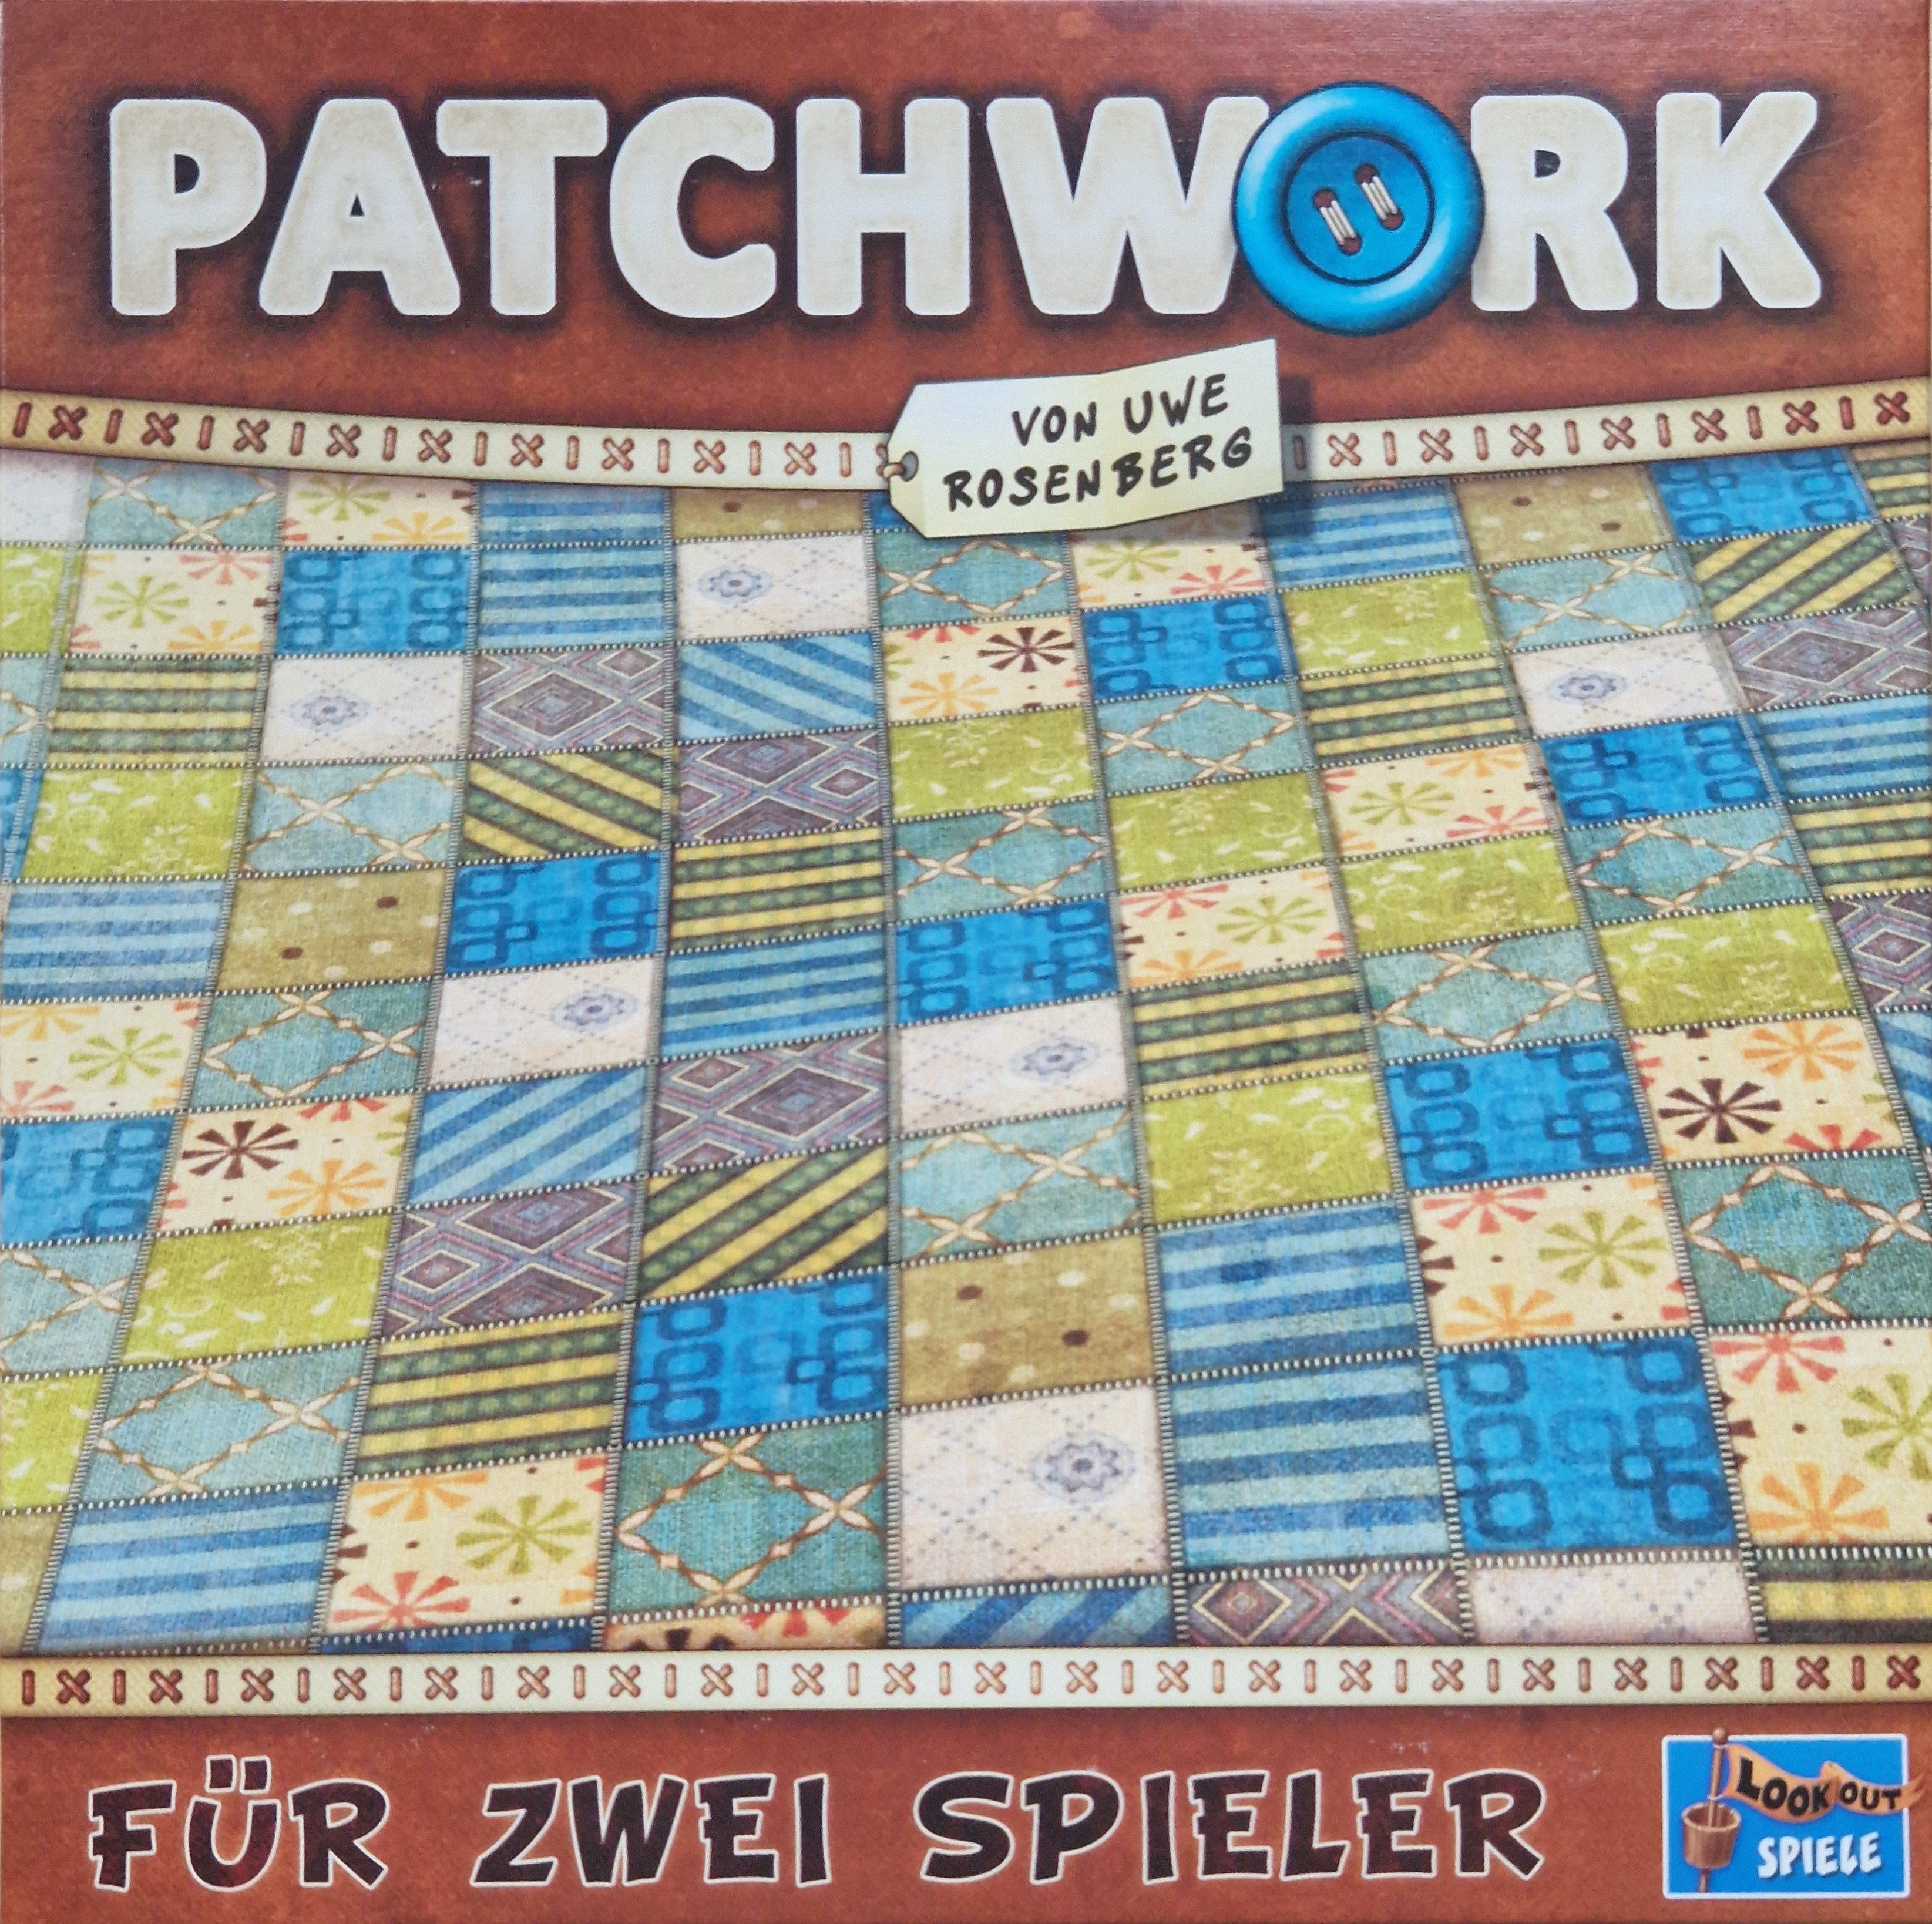
\includegraphics[width=0.28\textwidth]{res/pictures/assets/patchwork-cover.png}
    \caption[Cover von Patchwork]{\unskip}
    Cover von Patchwork
    \label{fig:patchwork-cover}
    \vspace*{-0.75cm}
\end{wrapfigure}

Patchwork ist ein Brettspiel von Uwe Rosenberg, das 2014 bei Lookout Spiele erschienen ist. Bei dem Brettspiel spielen zwei Spieler vom Alter 8 Jahre und aufwärts gegeneinander, wobei ein Spiel in der Regel ungefähr 30 Minuten lang ist \cite{LookoutSpielePatchwork}. Bei dem Brettspiel gestalten zwei Spieler jeweils eine eigne Decke aus Stoffresten, Flicken und Knöpfen, der Technik entsprechend, die der Titel vorgibt. \cite{SpielDesJahresPatchwork}

Das Ziel der Spieler ist mit den gegebenen Stoffplättchen unterschiedlicher Formen und Größen die vorgegebene Fläche zu füllen. Das Puzzlespiel erfordert taktisches Gespür, da die Flickenauswahl die Zugfolge und auch die Flickenauswahl des Gegenspielers beeinflusst. Immer können die Spieler jedoch nicht die gewünschten Flicken verwenden, da diese mit der Spielwährung Knöpfe aus der eigenen Kasse bezahlt werden müssen. An die begehrten Knöpfe kommen die Spieler über die bereits eingearbeiteten Flicken, welche Knöpfe auf sich abgebildet haben. Je mehr dieser Knöpfe auf der eigenen Decke abgebildet sind, desto höher das Einkommen an Knöpfen. Wer am Schluss des Spiels die meisten Knöpfe erwirtschaftet und seine Decke gut bestickt hat, gewinnt den Nähwettstreit. \cite{SpielDesJahresPatchwork}

\section{Spieltheorie}
\label{chapter:spieltheorie}

TODO:

\subsection{Spielbaum}

TODO: Spielbaum, Entscheidungsbaum

\subsection{Spielkomplexität}

TODO:

\begin{itemize}
    \item \textbf{Zustandsraum-Komplexität}: TODO:
    \item \textbf{Spielbaumgröße}: TODO:
    \item \textbf{Entscheidungskomplexität}: TODO: needed?
    \item \textbf{Spielbaumkomplexität}: TODO:
\end{itemize}

\section{Lineare Programmierung}
\label{chapter:lineare-programmierung}

TODO:

\section{Minimax-Algorithmus}
\label{chapter:minimax-algorithmus}

TODO:

Hier haben wir mehr

\section{Monte Carlo Tree Search}
\label{chapter:monte-carlo-tree-search}

\acf{MCTS} ist ein Suchalgorithmus, welcher verwendet wird, um in einem Spiel die beste Aktion zu finden. Dazu wird der Algorithmus während der Entscheidungszeit des Computerspielers ausgeführt. Innerhalb dieser Zeit wird schrittweise ein Suchbaum erstellt. Dabei wird für jede Aktion eine Heuristik erstellt, indem sehr viele Spiele zufällig bis zum Ende ausgespielt werden. Dadurch ergibt sich über die Zeit eine Wahrscheinlichkeit für das Ergebnis des Spiels für jede mögliche Aktion \cite[S. 61]{2008.ParallelMCTS}. Der \ac{MCTS}-Suchprozess besteht aus vier Phasen:

\begin{enumerate}
    \item \textbf{Selektion}: Der Suchbaum wird beginnend ab dem Wurzelknoten bis zu einem Blattknoten durchlaufen, indem in jeder Ebene immer genau ein Kindknoten nach einer bestimmten Richtlinie ausgewählt wird. \cite[S. 187]{2018.ReinforcementLearning}
    \item \textbf{Expansion}: Der ausgewählte Blattknoten wird um ein weiteres Kind erweitert, indem ein noch nicht erforschte Aktion ausgeführt wird. \cite[S. 61]{2008.ParallelMCTS}
    \item \textbf{Simulation}: Ausgehend vom neu hinzugefügten Knoten wird das Spiel bis zum Ende simuliert, indem bis Spielende zufällige Aktionen ausgeführt werden. \cite[S. 61]{2008.ParallelMCTS}
    \item \textbf{Backpropagation}: Das Ergebnis der Simulation wird durch den Suchbaum rückpropagiert, indem das Ergebnis (Gewonnen oder Verloren) ausgehend von dem in Zweitens neu hinzugefügten Knoten bis zum Wurzelknoten hochgereicht wird. \cite[S. 187]{2018.ReinforcementLearning}
\end{enumerate}

Die vier Phasen sind anschaulich in Abbildung \ref{fig:mcts-phases} dargestellt. Diese Phasen werden so lange wiederholt, bis die Entscheidungszeit vorbei ist.

\begin{figure}[!ht]
    \centering
    
\includegraphics[width=\textwidth]{res/pictures/mcts-phases.pdf}
    \caption{Phasen des \acs{MCTS} Algorithmus}
    \label{fig:mcts-phases}
\end{figure}

Für die erste Phase der Selektion wird im Normalfall die in \ref{eqn:uct} dargestellte \ac{UCT} Formel verwendet. Die \ac{UCT} Formel balanciert die Entscheidung zwischen der Ausnutzung von bereits bekannten Aktionen mit der Erkundung von unsicheren Aktionen \cite[S. 206]{2009.ComputerGoMCTS}. Dazu wird im ersten Teil die Anzahl der Siege ($w$) durch die Anzahl der Besuche des Kindknotens ($n$) geteilt. Dieser Term wird immer größer, je öfters eine Simulation nach einem Knotenbesuch gewonnen wird. Der andere Term wird immer größer, je weniger ein Knoten im Vergleich zu seinem Elternknoten ($N$) besucht wird und erzwingt somit auch die Erkundung weniger besuchter Knoten. Bei $c$ handelt es sich um eine Erkundungskonstante, welche das Verhältnis zwischen Ausnutzung und Exploration regelt und normalerweise auf $\sqrt{2}$ gesetzt wird.

\begin{equation}
    \label{eqn:uct}
    \mathbb{U}\mathbb{C}\mathbb{T} = \frac{w}{n} + c \cdot \sqrt{\frac{\ln N}{n}}
\end{equation}

Ein entscheidender Vorteil von \ac{MCTS} ist, dass keine statische Evaluierungsfunktion einer Position wie bei vergleichbaren Algorithmen existieren muss \cite[S. 61]{2008.ParallelMCTS}, da durch zufällige Erkundungen eines Teils des Suchbaums eine Approximation für den tatsächlichen Wert geschaffen wird. \ac{MCTS} hat sich vor allem für Spiele mit einer sehr großen Anzahl an Aktionen bzw. möglichen Zuständen als besser geeignet als traditionelle \hyperref[chapter:minimax-algorithmus]{Minimax}-basierte Programme herausgestellt \cite[S. 1]{2013.MCTSAndMinimaxHybrids} und ist aus diesem Grund auch zu großen Teilen für die Verbesserung der Computergegner in solchen Spielen wie beispielsweise Go verantwortlich \cite[S. 2006]{2009.ComputerGoMCTS} \cite[S. 185]{2018.ReinforcementLearning}.

\section{AlphaZero}
\label{chapter:alphazero}

TODO:

\section{Interaktive Systeme}
\label{chapter:interaktive-systeme}

TODO:


\chapter{Analyse des Brettspiels}
\label{chapter:analyse-des-bretspiels}

TODO:


\chapter{Umsetzung}
\label{chapter:umsetzung}

TODO:
\chapter{Evaluation}
\label{chapter:evaluation}

TODO:
\chapter{Fazit}
\label{chapter:fazit}

TODO:

% ---- Literaturverzeichnis
\cleardoublepage
\renewcommand*{\chapterpagestyle}{plain}
\pagestyle{plain}
\pagenumbering{Roman}                   % Römische Seitenzahlen
\setcounter{page}{\numexpr\value{savepage}+1}
\printbibliography[title=Literaturverzeichnis]

% ---- Anhang
\appendix
\clearpage
\pagenumbering{Roman}  % römische Seitenzahlen für Anhang
\chapter{Anhangskapitel}
\label{anhang:chapter-anhangskapitel}

TODO:

Tabelle/Text mit Patchwork Terminologie

\pagebreak

\chapter{Patchwork}

% \section{Patchwork \textemdash Terminologie}

% TODO:

\section{Zeitpläne}

\begin{figure}[!ht]
    \centering
    \begin{minipage}{.48\textwidth}
        \centering
        \begin{tikzpicture}
            \node [inner sep=0pt,,outer sep=0pt,clip,rounded corners=0.15cm] (image) at (0,0) {\includegraphics[width=0.75\linewidth]{res/pictures/assets/time-board-side-1.png}};
            \drawshadow{image}
        \end{tikzpicture}
    \end{minipage}
    \hfill
    \begin{minipage}{.48\textwidth}
        \centering
        \begin{tikzpicture}
            \node [inner sep=0pt,,outer sep=0pt,clip,rounded corners=0.15cm] (image) at (0,0) {\includegraphics[width=0.75\linewidth]{res/pictures/assets/time-board-side-2.png}};
            \drawshadow{image}
        \end{tikzpicture}
    \end{minipage}
    \vspace*{-0.05cm}
    \caption{Die zwei Seiten des Zeitplans}
    \label{fig:patchwork-time-board}
\end{figure}

\section{Ablagepläne}

\begin{figure}[!ht]
    \centering
    \begin{minipage}{.48\textwidth}
        \centering
        \begin{tikzpicture}
            \node [inner sep=0pt,,outer sep=0pt,clip,rounded corners=0.15cm] (image) at (0,0) {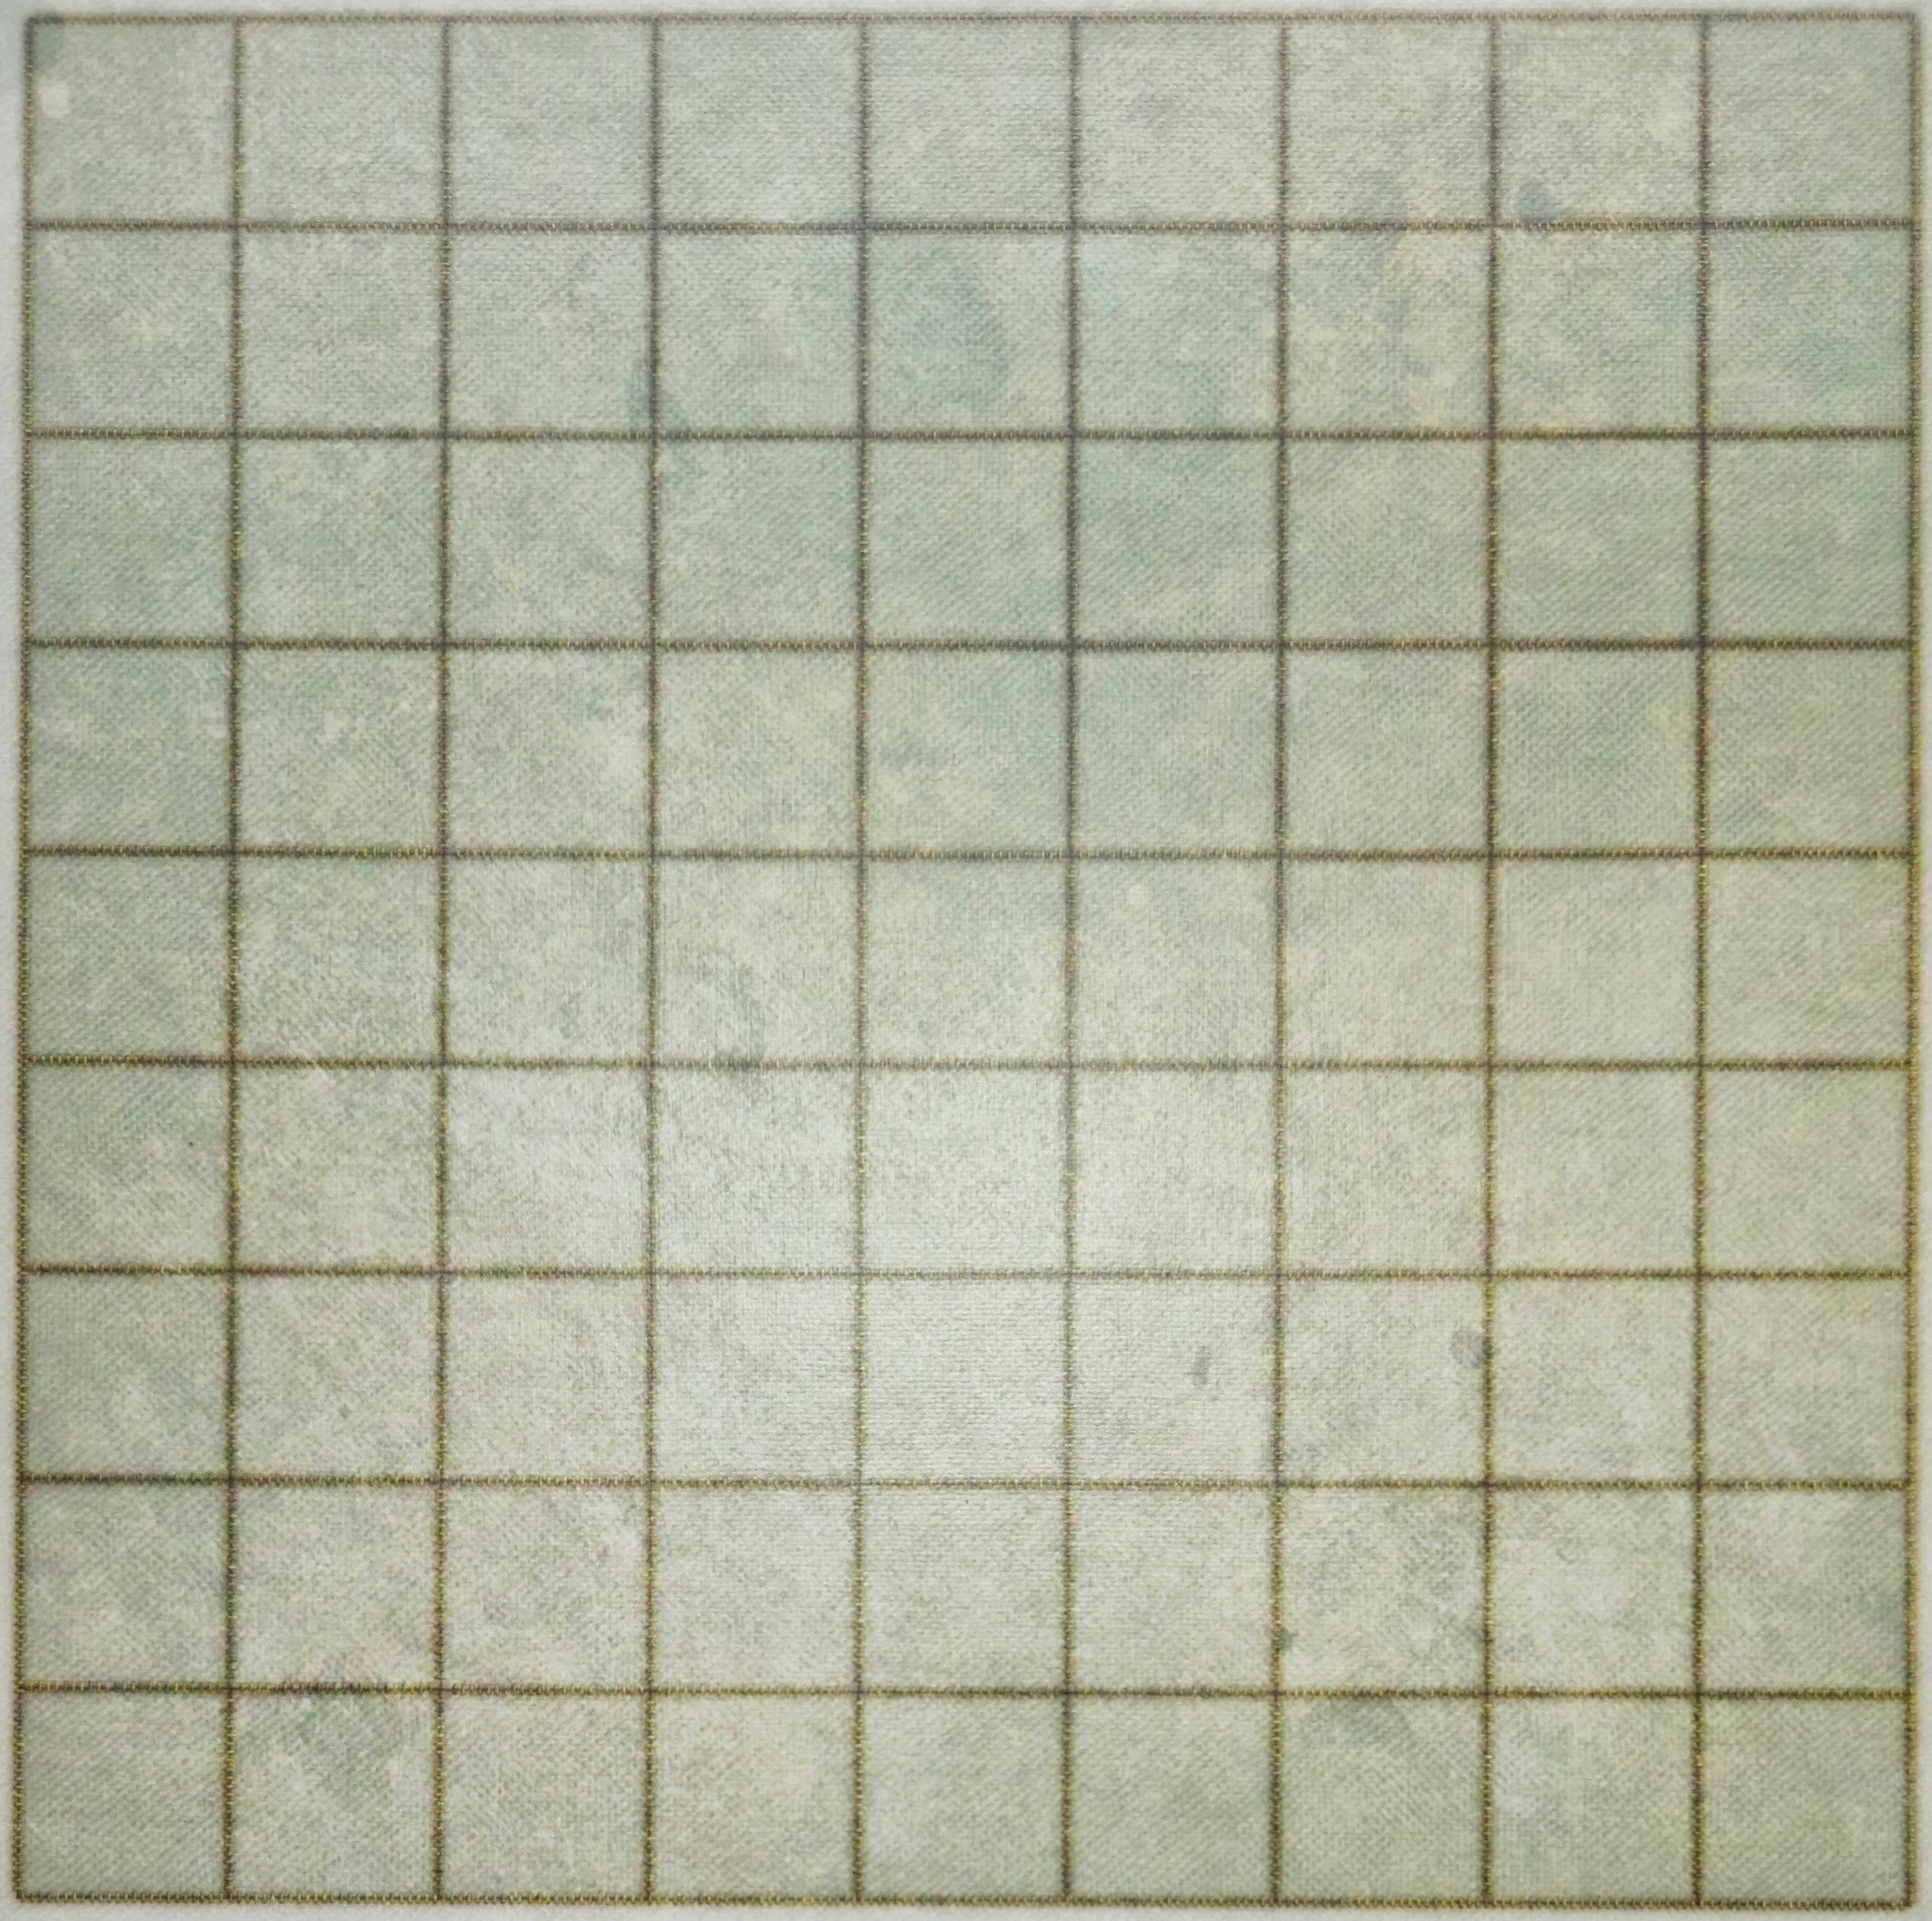
\includegraphics[width=0.75\linewidth]{res/pictures/assets/board-player-1.png}};
            \drawshadow{image}
        \end{tikzpicture}
    \end{minipage}
    \hfill
    \begin{minipage}{.48\textwidth}
        \centering
        \begin{tikzpicture}
            \node [inner sep=0pt,,outer sep=0pt,clip,rounded corners=0.15cm] (image) at (0,0) {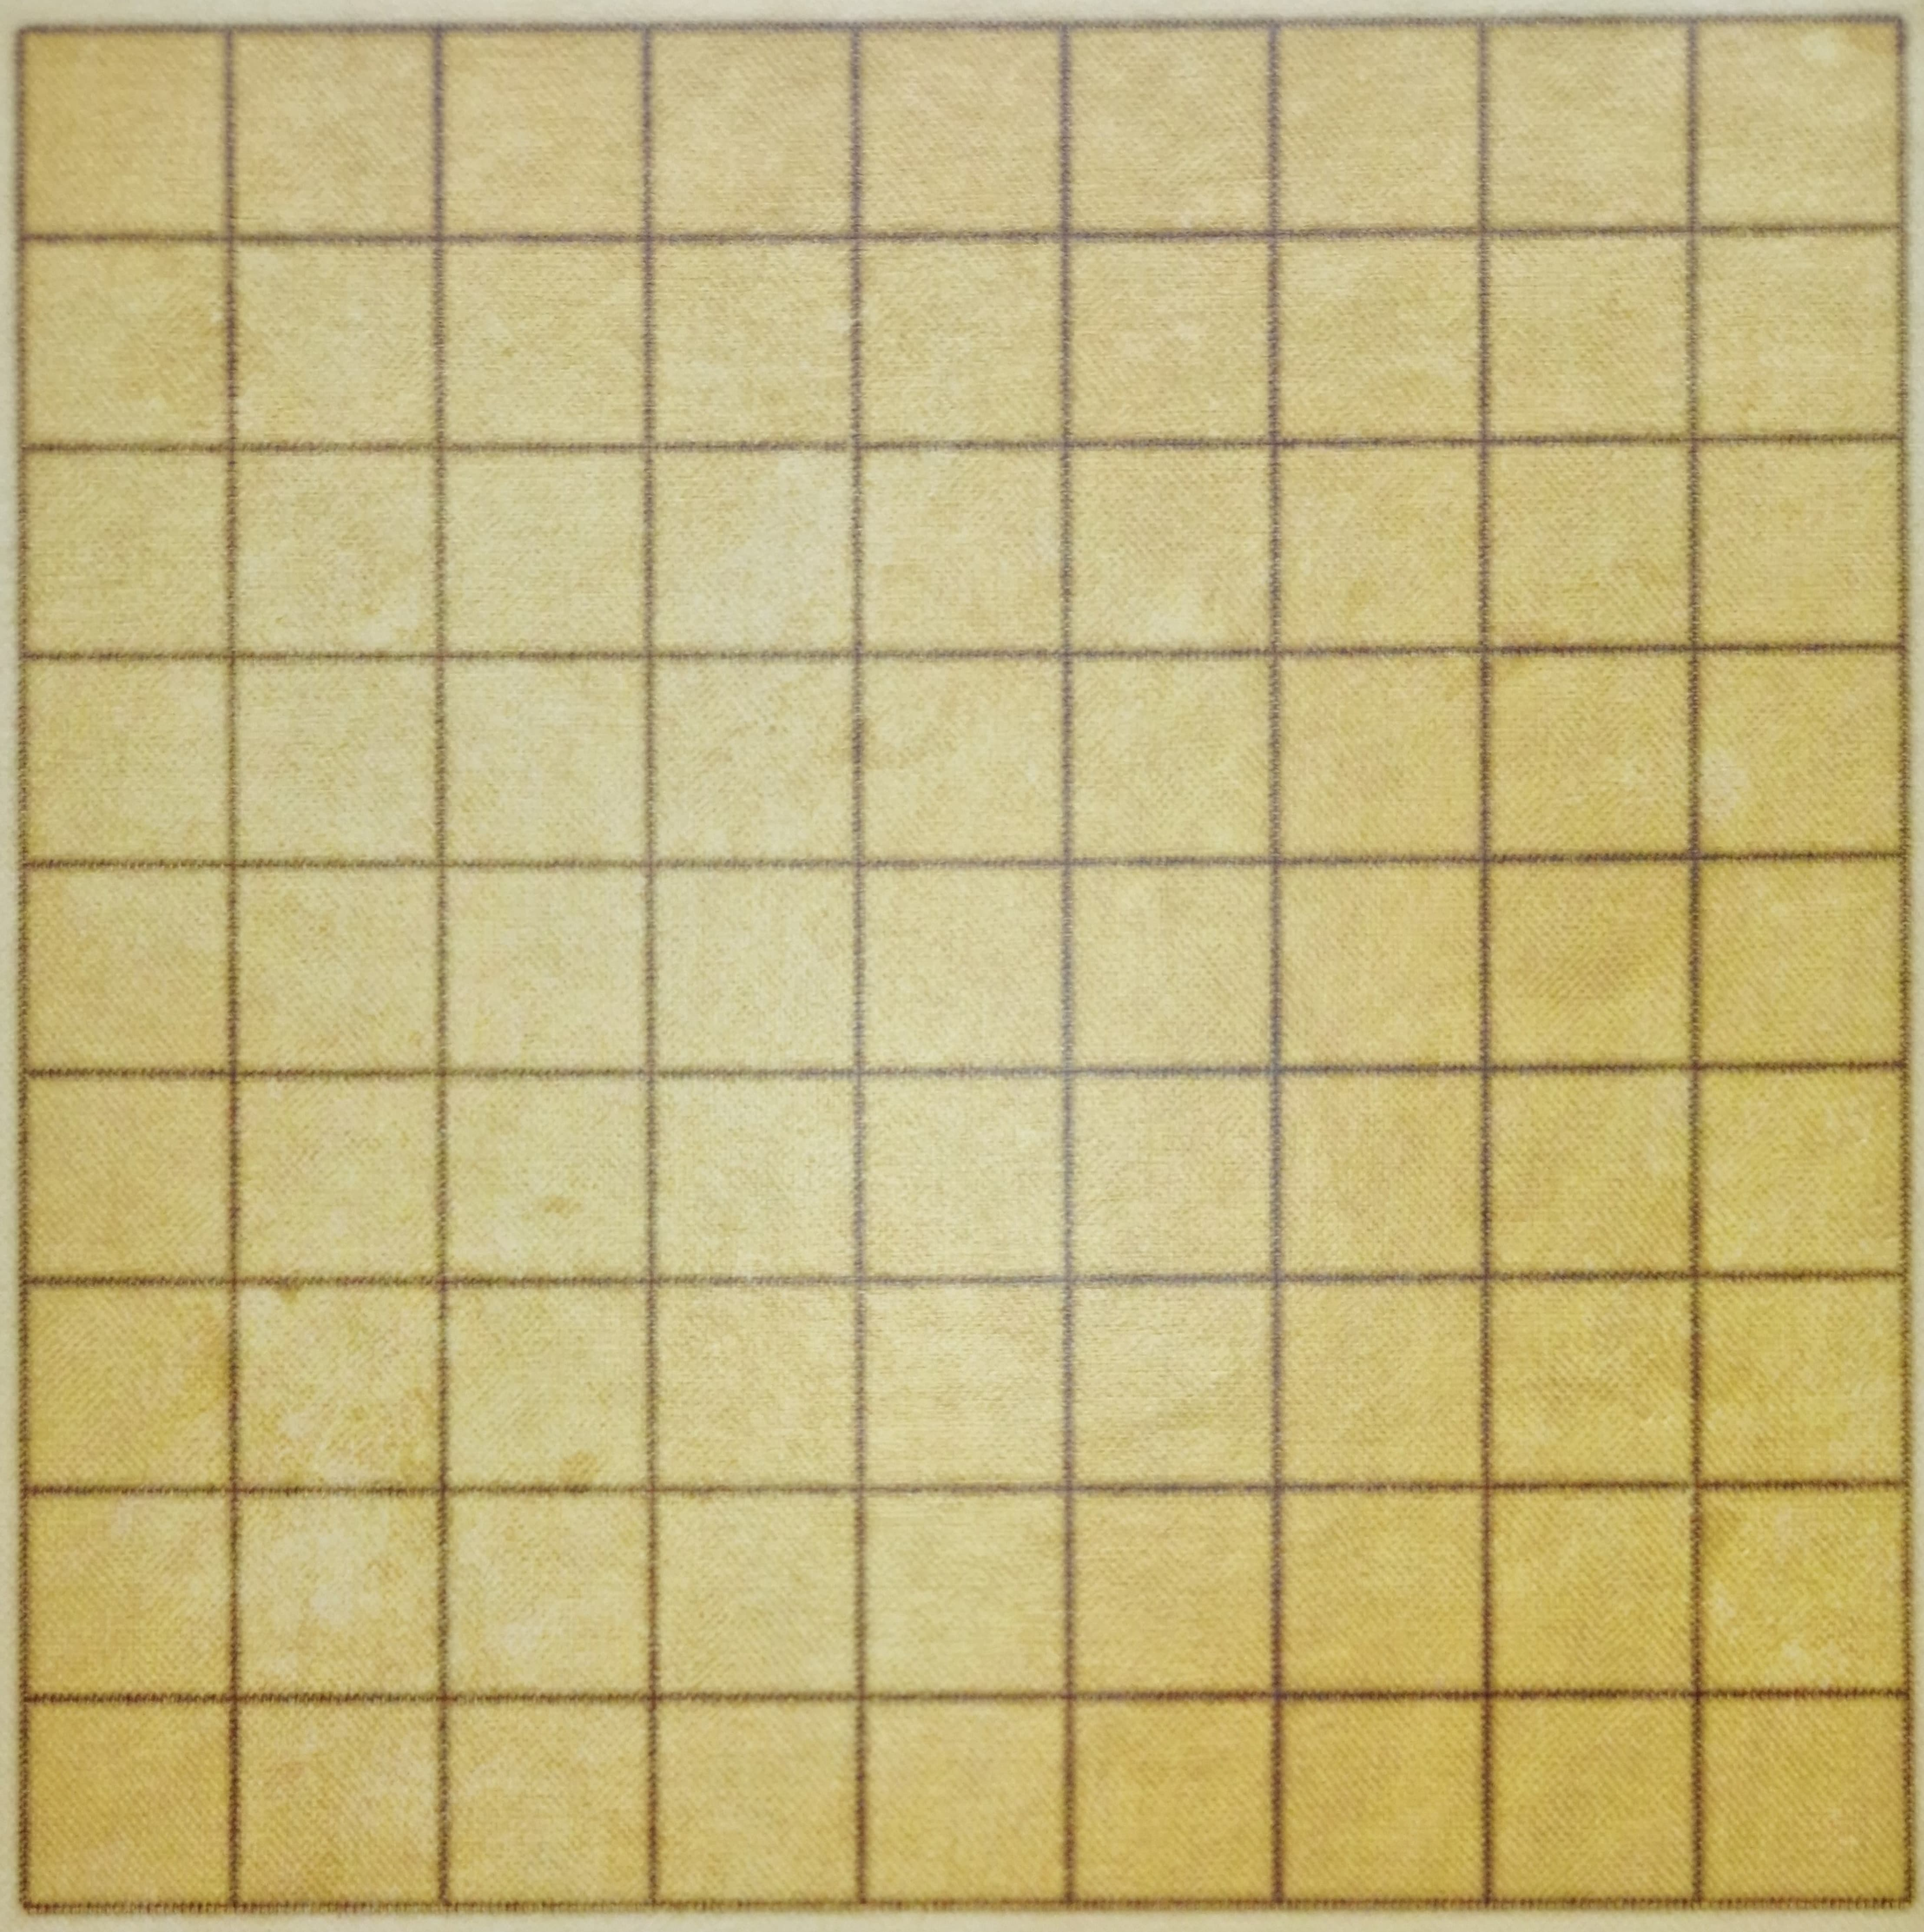
\includegraphics[width=0.75\linewidth]{res/pictures/assets/board-player-2.png}};
            \drawshadow{image}
        \end{tikzpicture}
    \end{minipage}
    \vspace*{-0.05cm}
    \caption{Ablagepläne (Decken) der Spieler}
    \label{fig:patchwork-player-quilt-board}
\end{figure}

\pagebreak

\section{Flicken}
\label{anhang:section-patchwork-patches}

% \setlength{\tabcolsep}{5pt}

\begin{longtable}[t]{|c|c|c|c|c|c|c|}
    \hline
    \raisebox{0pt}[3ex][2ex]{Flicken}                                                                                                                 & ID   & Felder & \makecell{ Knopf                                              \\ Kosten } & \makecell{ Zeit \\ Kosten } & \makecell{ Knopf \\ Einkommen } & $\frac{\text{Knopfeinkommen}}{\text{Felder}\, \cdot\, \text{Zeitkosten}}$ \\ \hline
    \endfirsthead
    \multicolumn{7}{c}{\tablename\ \thetable\ -- \textit{Fortsetzung von der vorherigen Seite}}                                                                                                                                       \\
    \hline
    \raisebox{0pt}[3ex][2ex]{Flicken}                                                                                                                 & ID   & Felder & \makecell{ Knopf                                              \\ Kosten } & \makecell{ Zeit \\ Kosten } & \makecell{ Knopf \\ Einkommen } & $\frac{\text{Knopfeinkommen}}{\text{Felder}\, \cdot\, \text{Zeitkosten}}$ \\ \hline
    \endhead
    \hline \multicolumn{7}{r}{\textit{Fortsetzung auf der nächsten Seite}}                                                                                                                                                            \\
    \endfoot
    \hline
    \caption{Alle 33 Flicken in Patchwork}
    \label{tabelle:patchwork-patches}
    \endlastfoot
    \adjustbox{valign=m, max width=0.2\textwidth, max height=0.1\textheight}{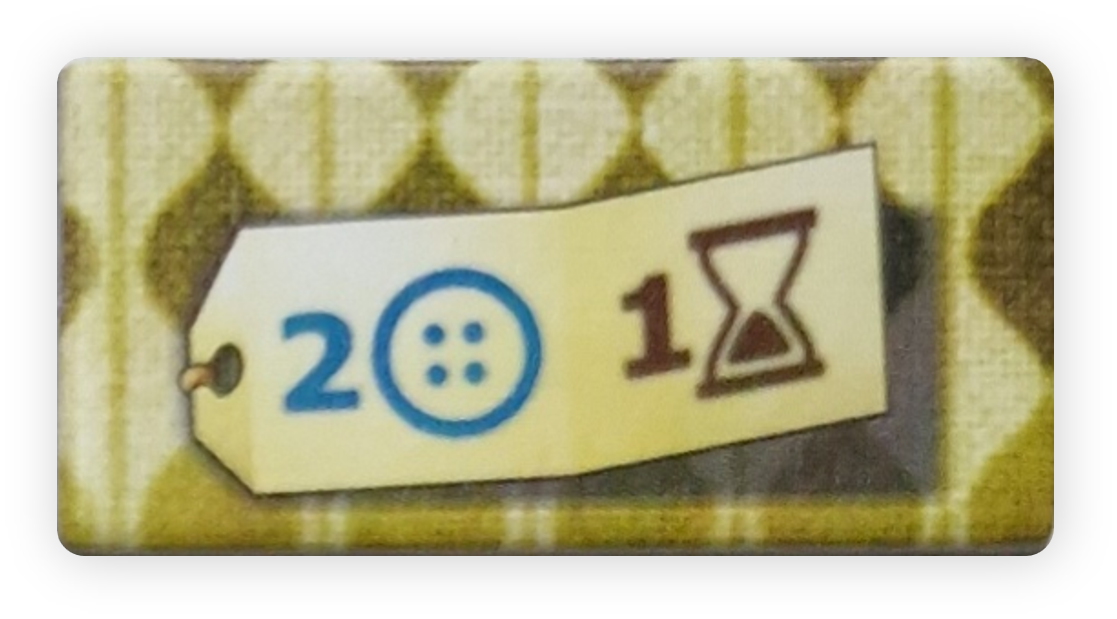
\includegraphics[width=0.2\textwidth]{res/pictures/assets/00-front.png}} & $0$  & $2$    & $2$              & $1$ & $0$ & $0$                            \\ \hline
    \adjustbox{valign=m, max width=0.2\textwidth, max height=0.1\textheight}{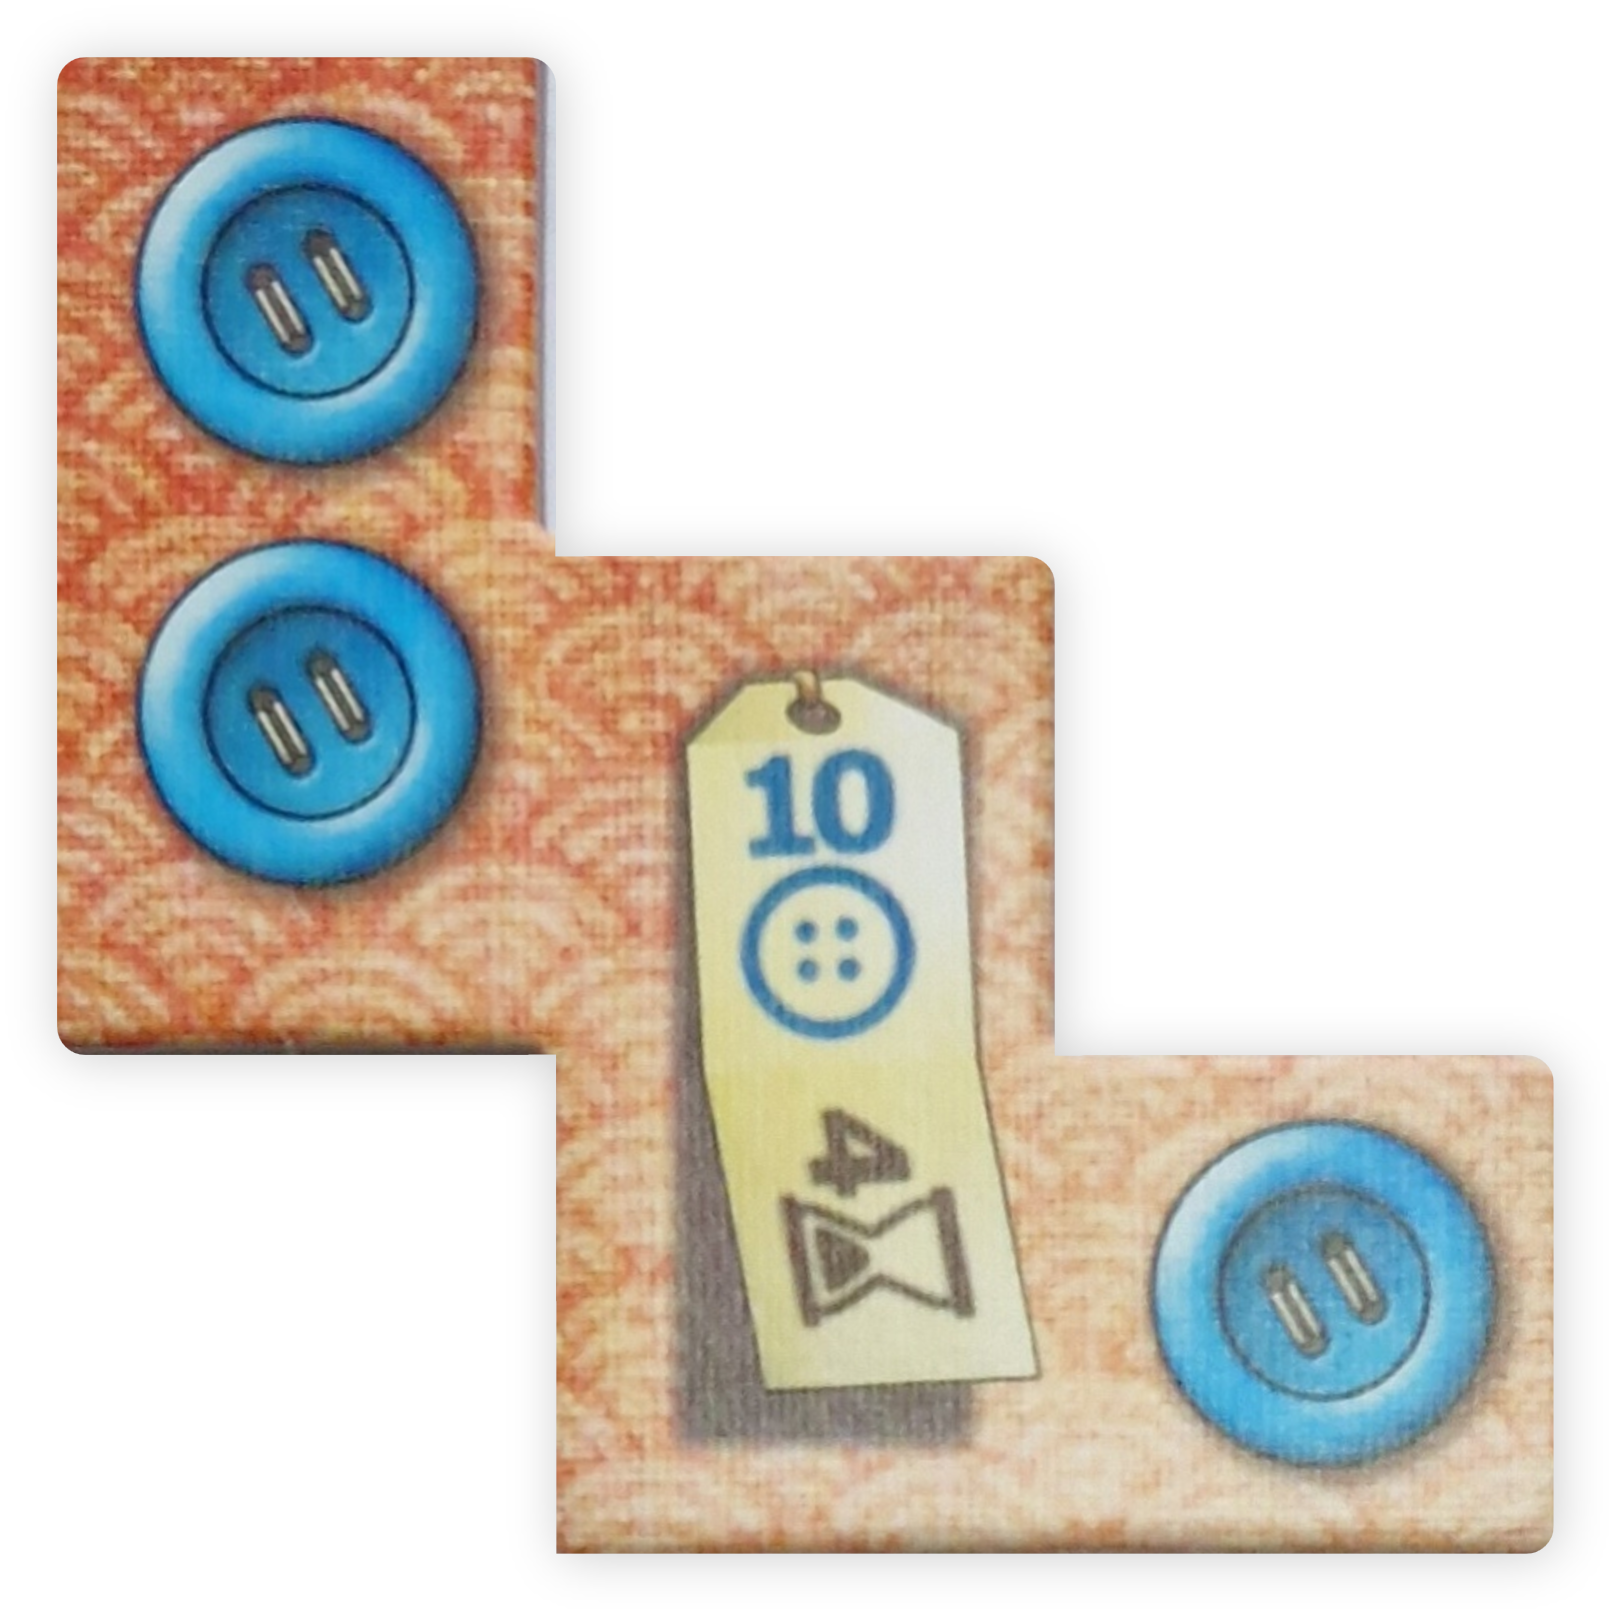
\includegraphics[width=0.2\textwidth]{res/pictures/assets/01-front.png}} & $1$  & $5$    & $10$             & $4$ & $3$ & $\frac{3}{20} = 0{,}15$        \\ \hline
    \adjustbox{valign=m, max width=0.2\textwidth, max height=0.1\textheight}{\includegraphics[width=0.2\textwidth]{res/pictures/assets/02-front.png}} & $2$  & $8$    & $5$              & $3$ & $1$ & $\frac{1}{24} \approx 0{,}042$ \\ \hline
    \adjustbox{valign=m, max width=0.2\textwidth, max height=0.1\textheight}{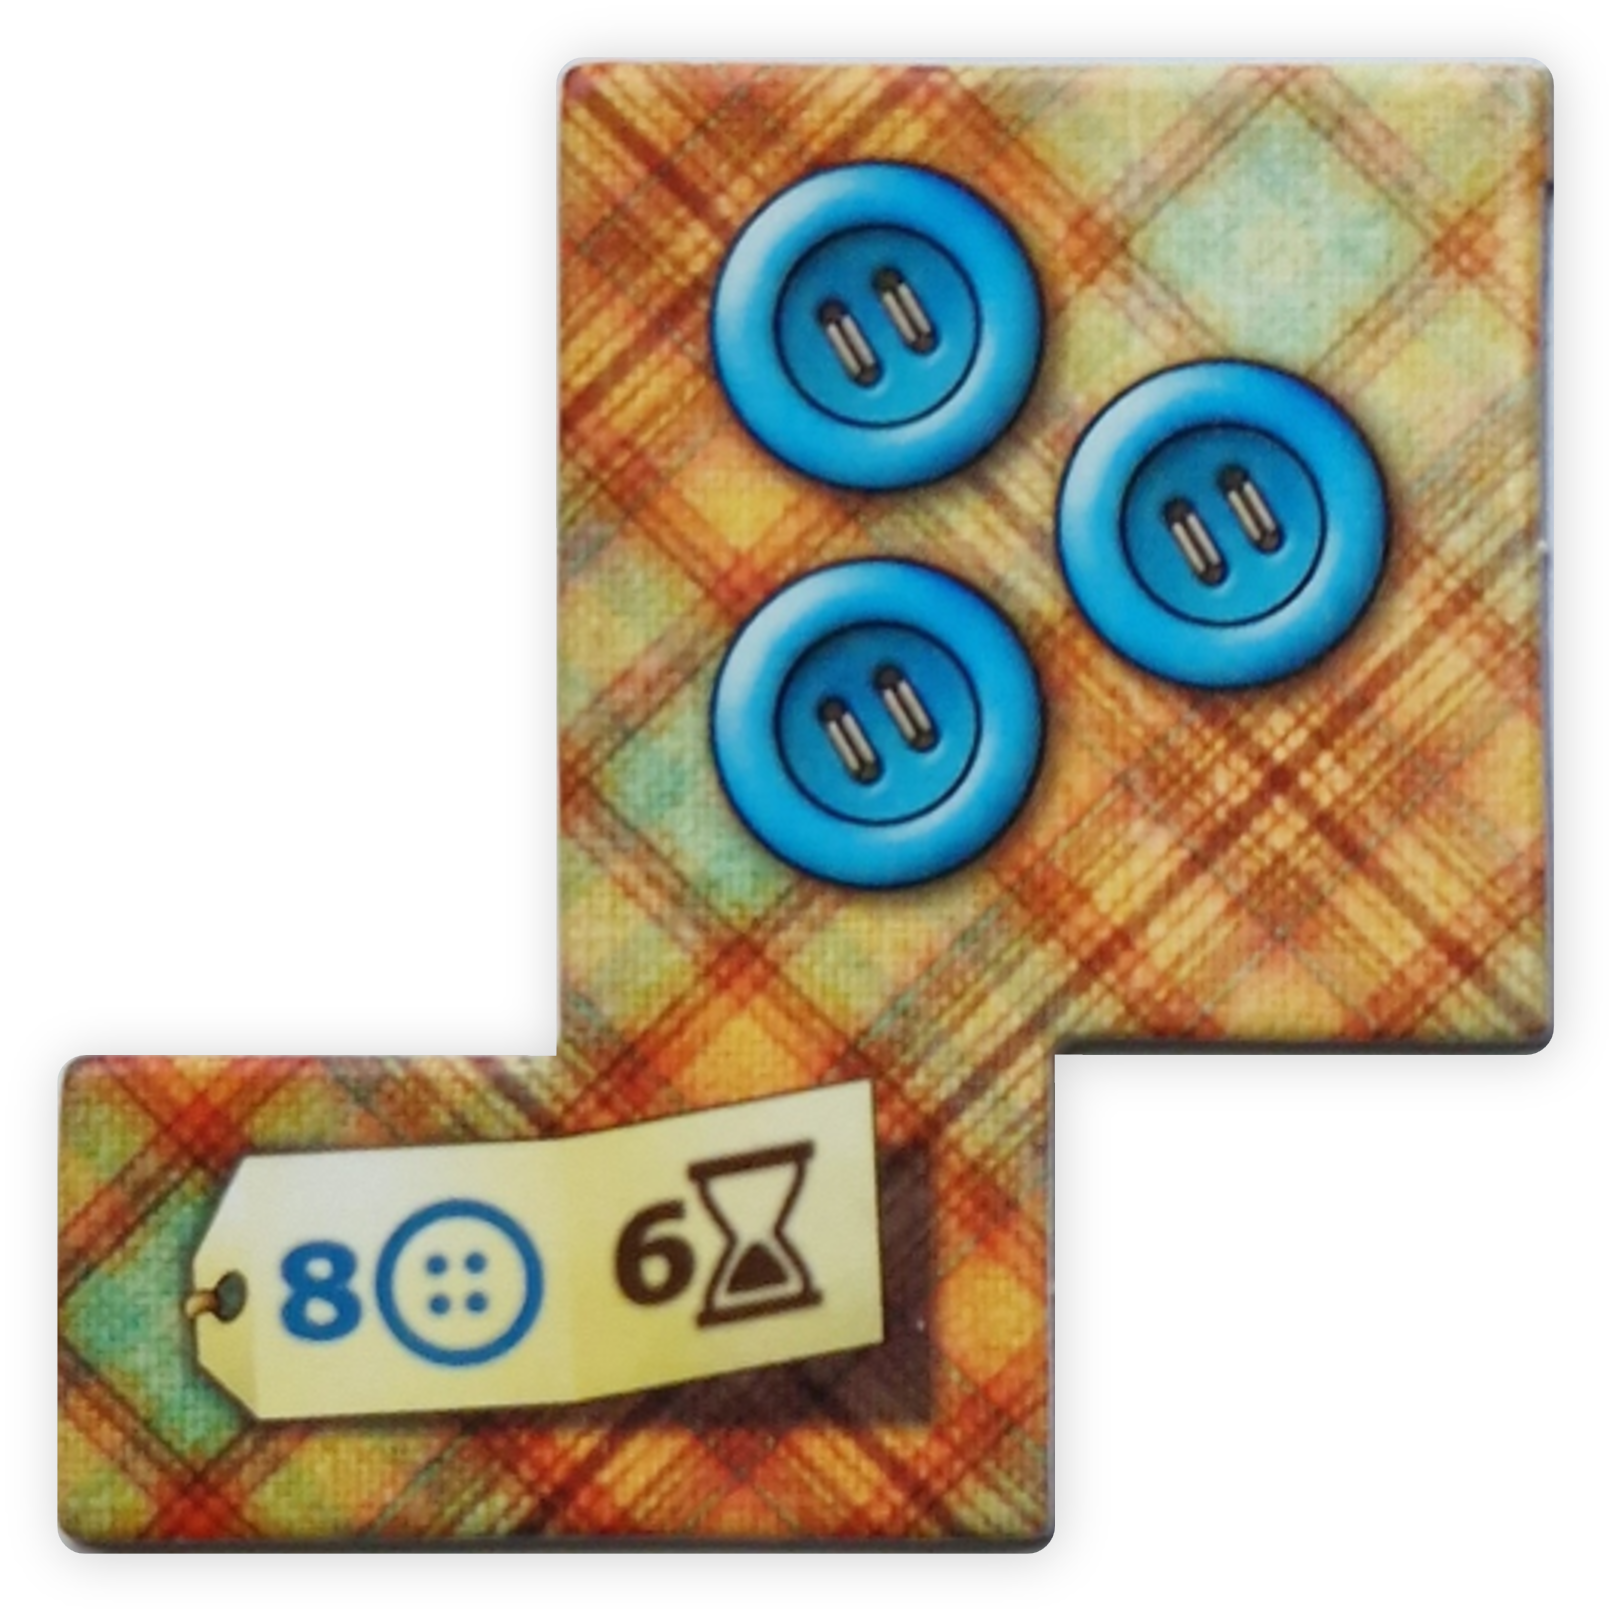
\includegraphics[width=0.2\textwidth]{res/pictures/assets/03-front.png}} & $3$  & $6$    & $8$              & $6$ & $3$ & $\frac{1}{12} \approx 0{,}083$ \\ \hline
    \adjustbox{valign=m, max width=0.2\textwidth, max height=0.1\textheight}{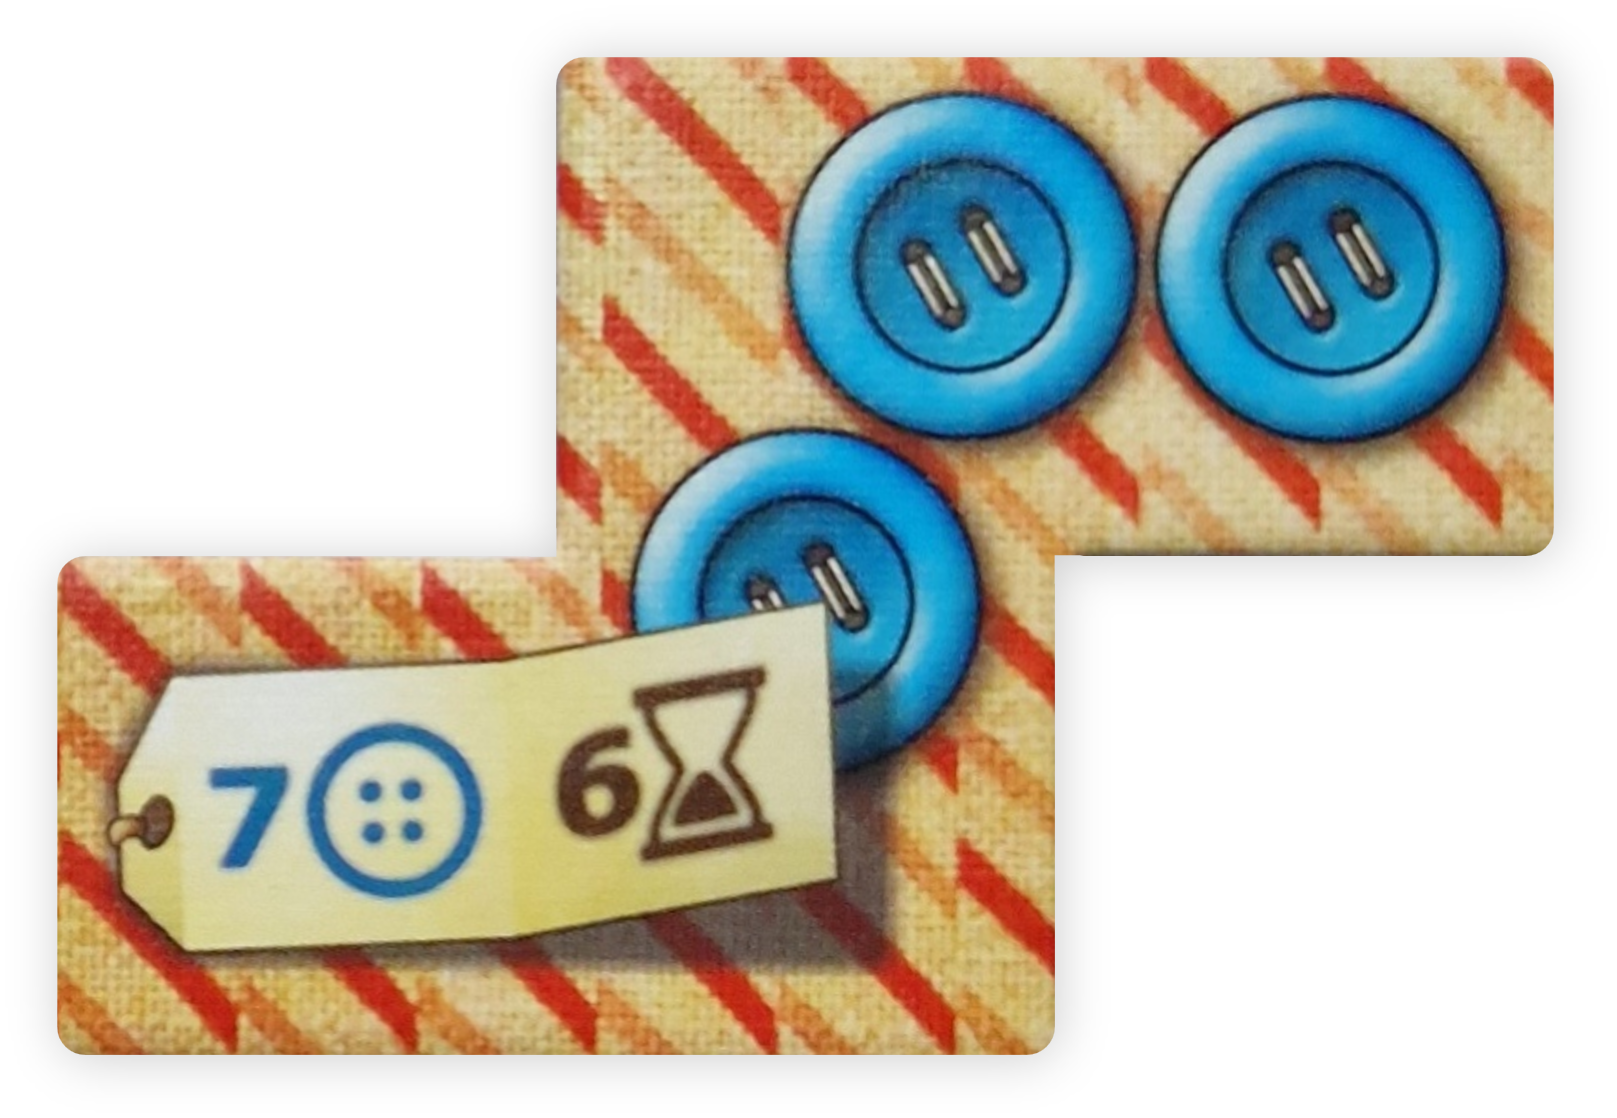
\includegraphics[width=0.2\textwidth]{res/pictures/assets/04-front.png}} & $4$  & $4$    & $7$              & $6$ & $3$ & $\frac{1}{8} = 0{,}125$        \\ \hline
    \adjustbox{valign=m, max width=0.2\textwidth, max height=0.1\textheight}{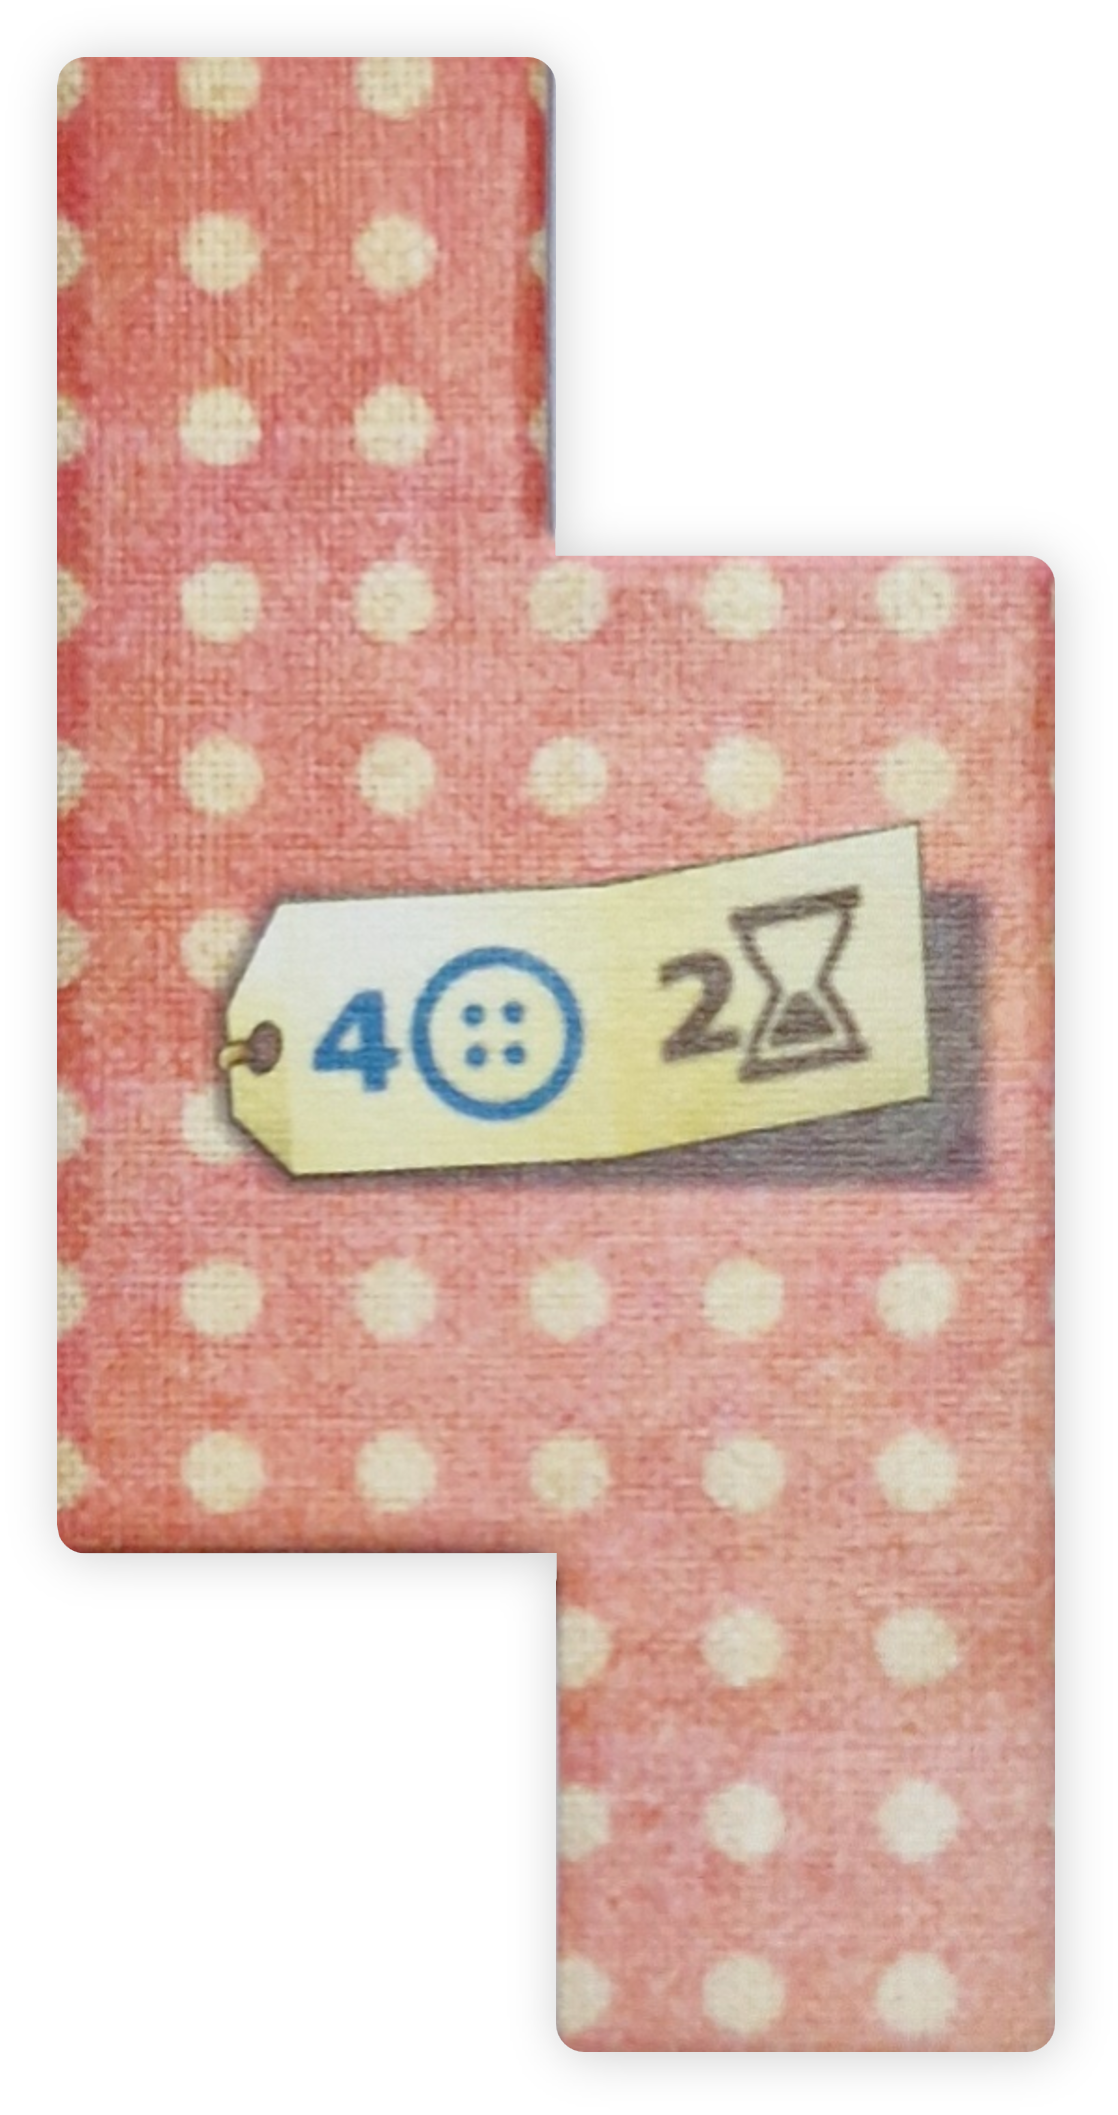
\includegraphics[width=0.2\textwidth]{res/pictures/assets/05-front.png}} & $5$  & $6$    & $4$              & $2$ & $0$ & $0$                            \\ \hline
    \adjustbox{valign=m, max width=0.2\textwidth, max height=0.1\textheight}{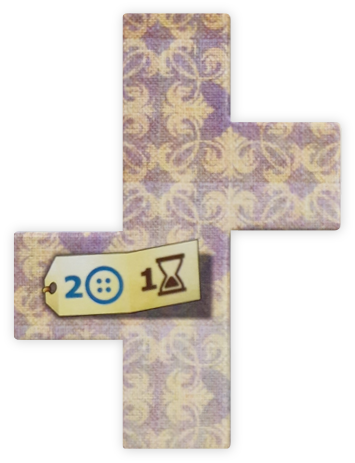
\includegraphics[width=0.2\textwidth]{res/pictures/assets/06-front.png}} & $6$  & $6$    & $2$              & $1$ & $0$ & $0$                            \\ \hline
    \adjustbox{valign=m, max width=0.2\textwidth, max height=0.1\textheight}{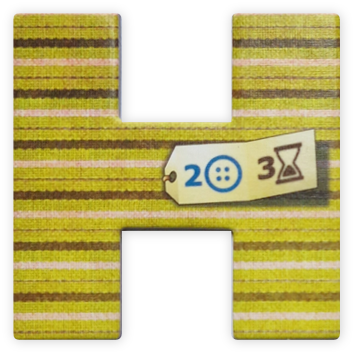
\includegraphics[width=0.2\textwidth]{res/pictures/assets/07-front.png}} & $7$  & $7$    & $2$              & $3$ & $0$ & $0$                            \\ \hline
    \adjustbox{valign=m, max width=0.2\textwidth, max height=0.1\textheight}{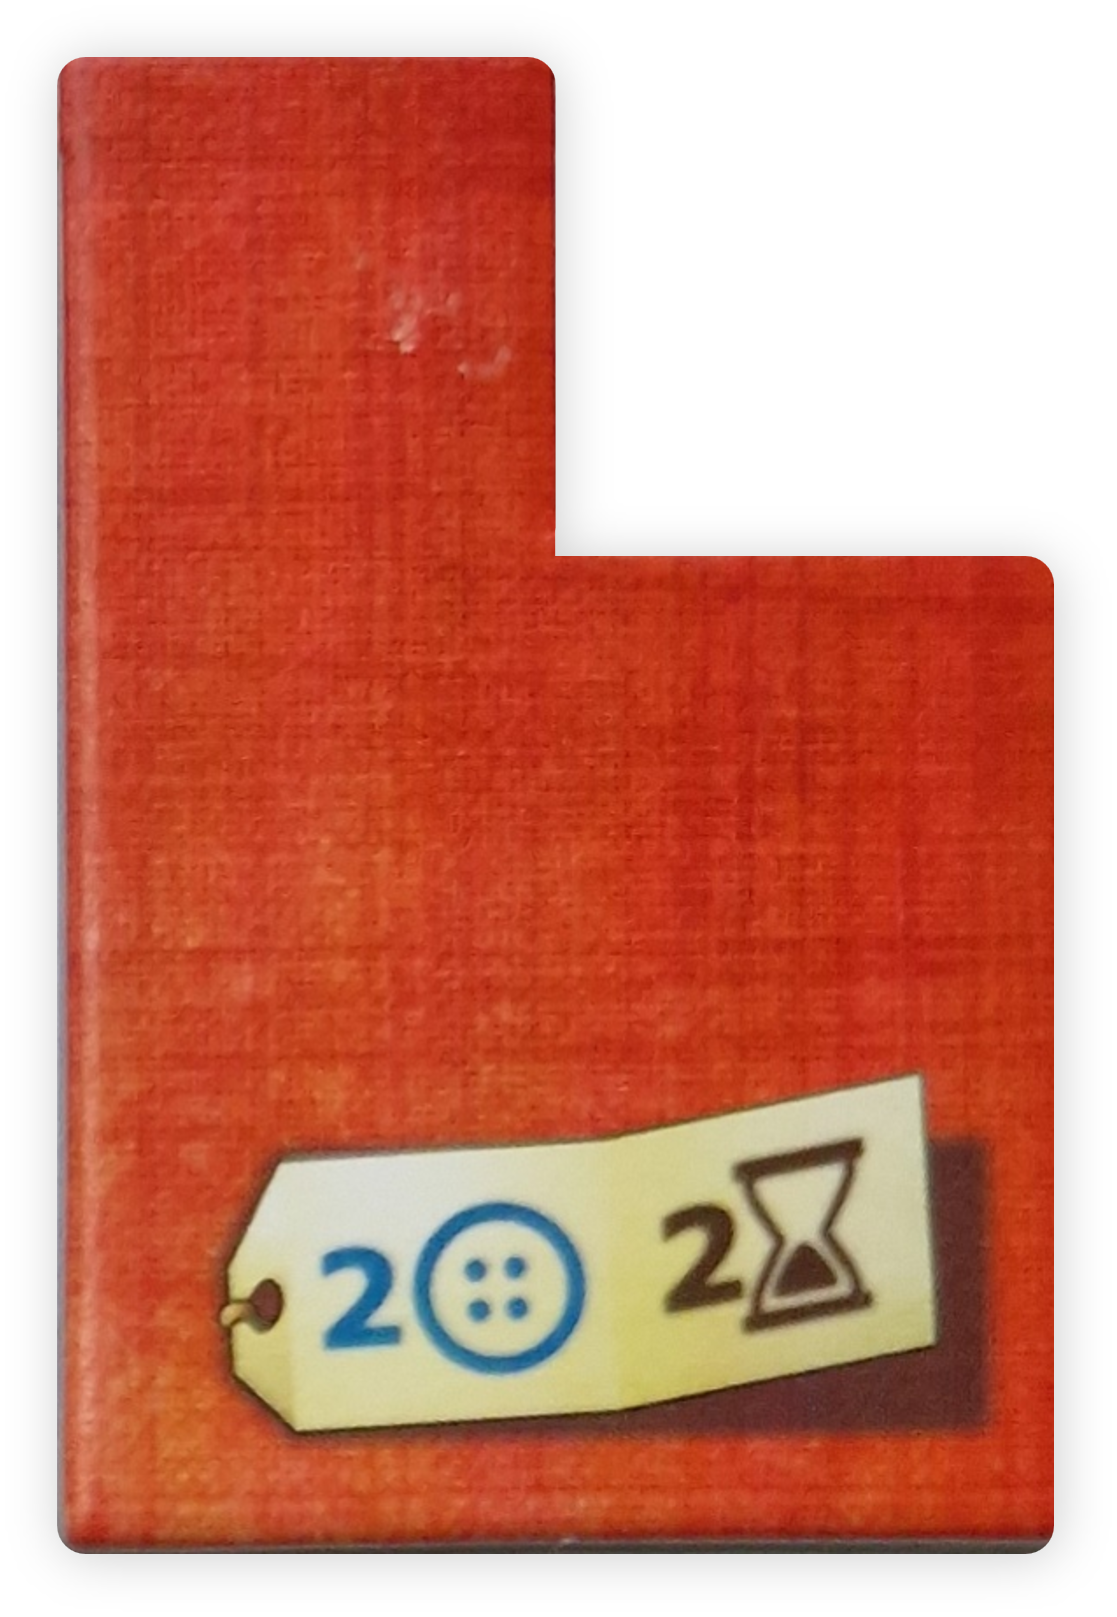
\includegraphics[width=0.2\textwidth]{res/pictures/assets/08-front.png}} & $8$  & $5$    & $2$              & $2$ & $0$ & $0$                            \\ \hline
    \adjustbox{valign=m, max width=0.2\textwidth, max height=0.1\textheight}{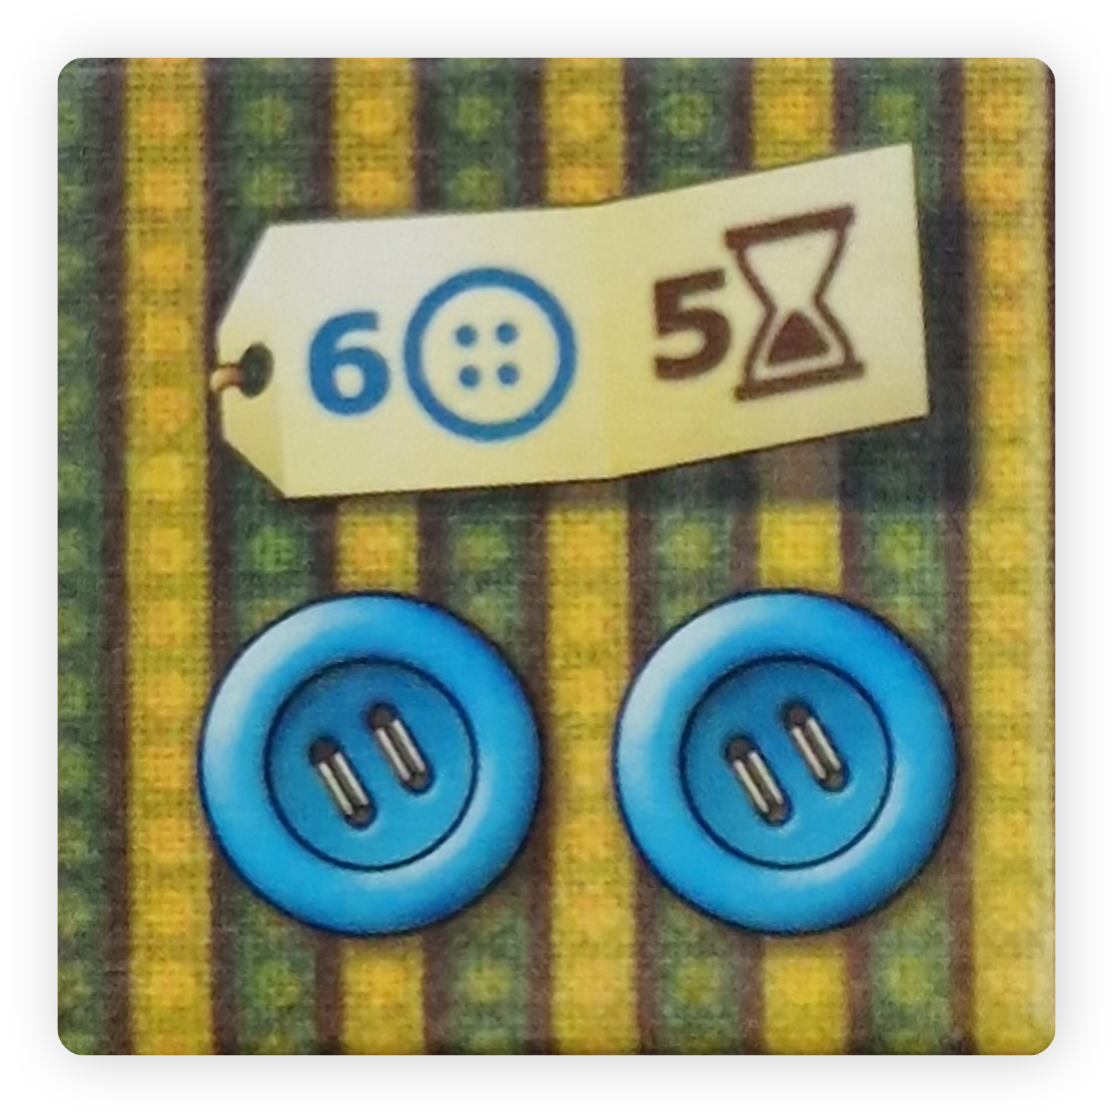
\includegraphics[width=0.2\textwidth]{res/pictures/assets/09-front.png}} & $9$  & $4$    & $6$              & $5$ & $2$ & $\frac{1}{10} = 0{,}1$         \\ \hline
    \adjustbox{valign=m, max width=0.2\textwidth, max height=0.1\textheight}{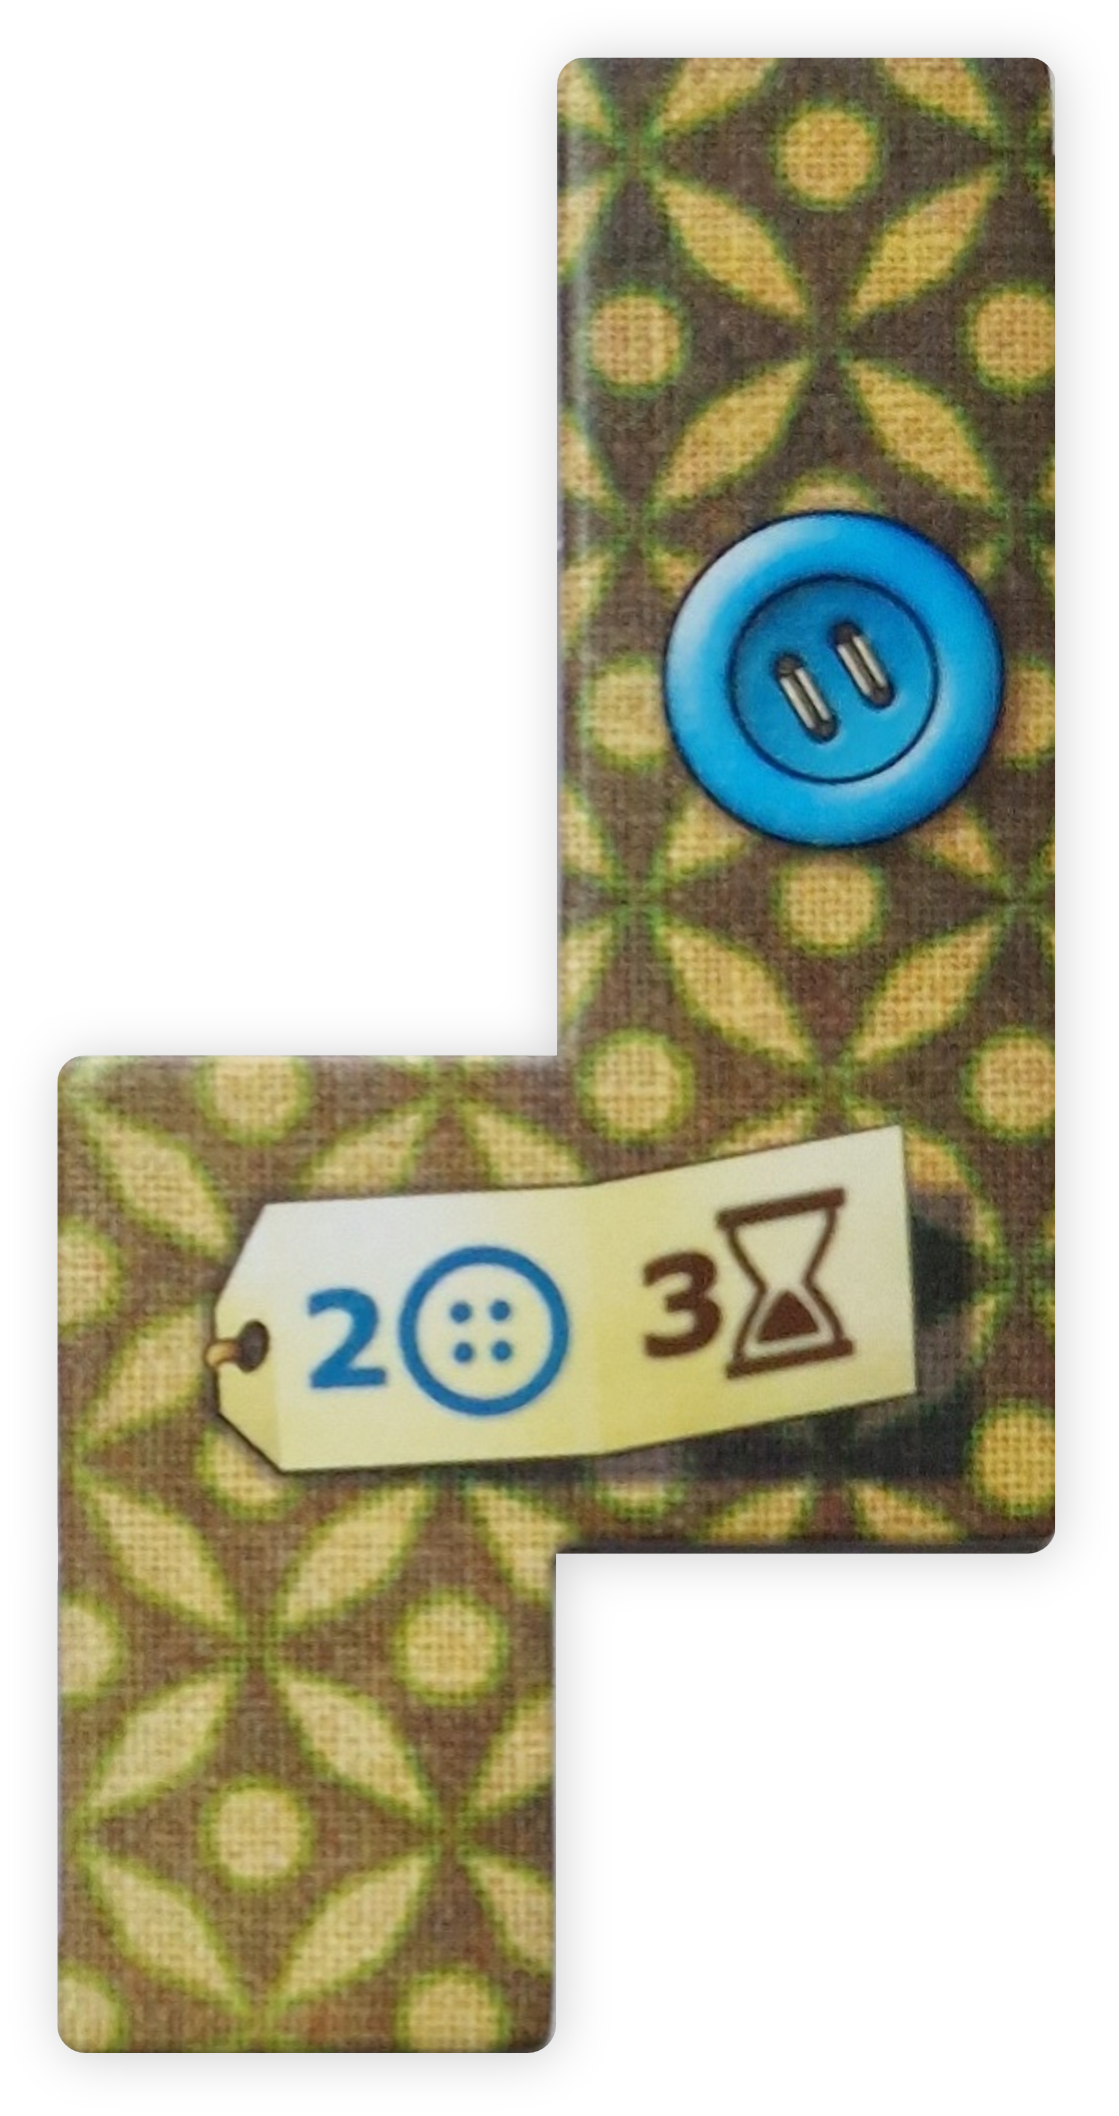
\includegraphics[width=0.2\textwidth]{res/pictures/assets/10-front.png}} & $10$ & $5$    & $2$              & $3$ & $1$ & $\frac{1}{15} \approx 0{,}067$ \\ \hline
    \adjustbox{valign=m, max width=0.2\textwidth, max height=0.1\textheight}{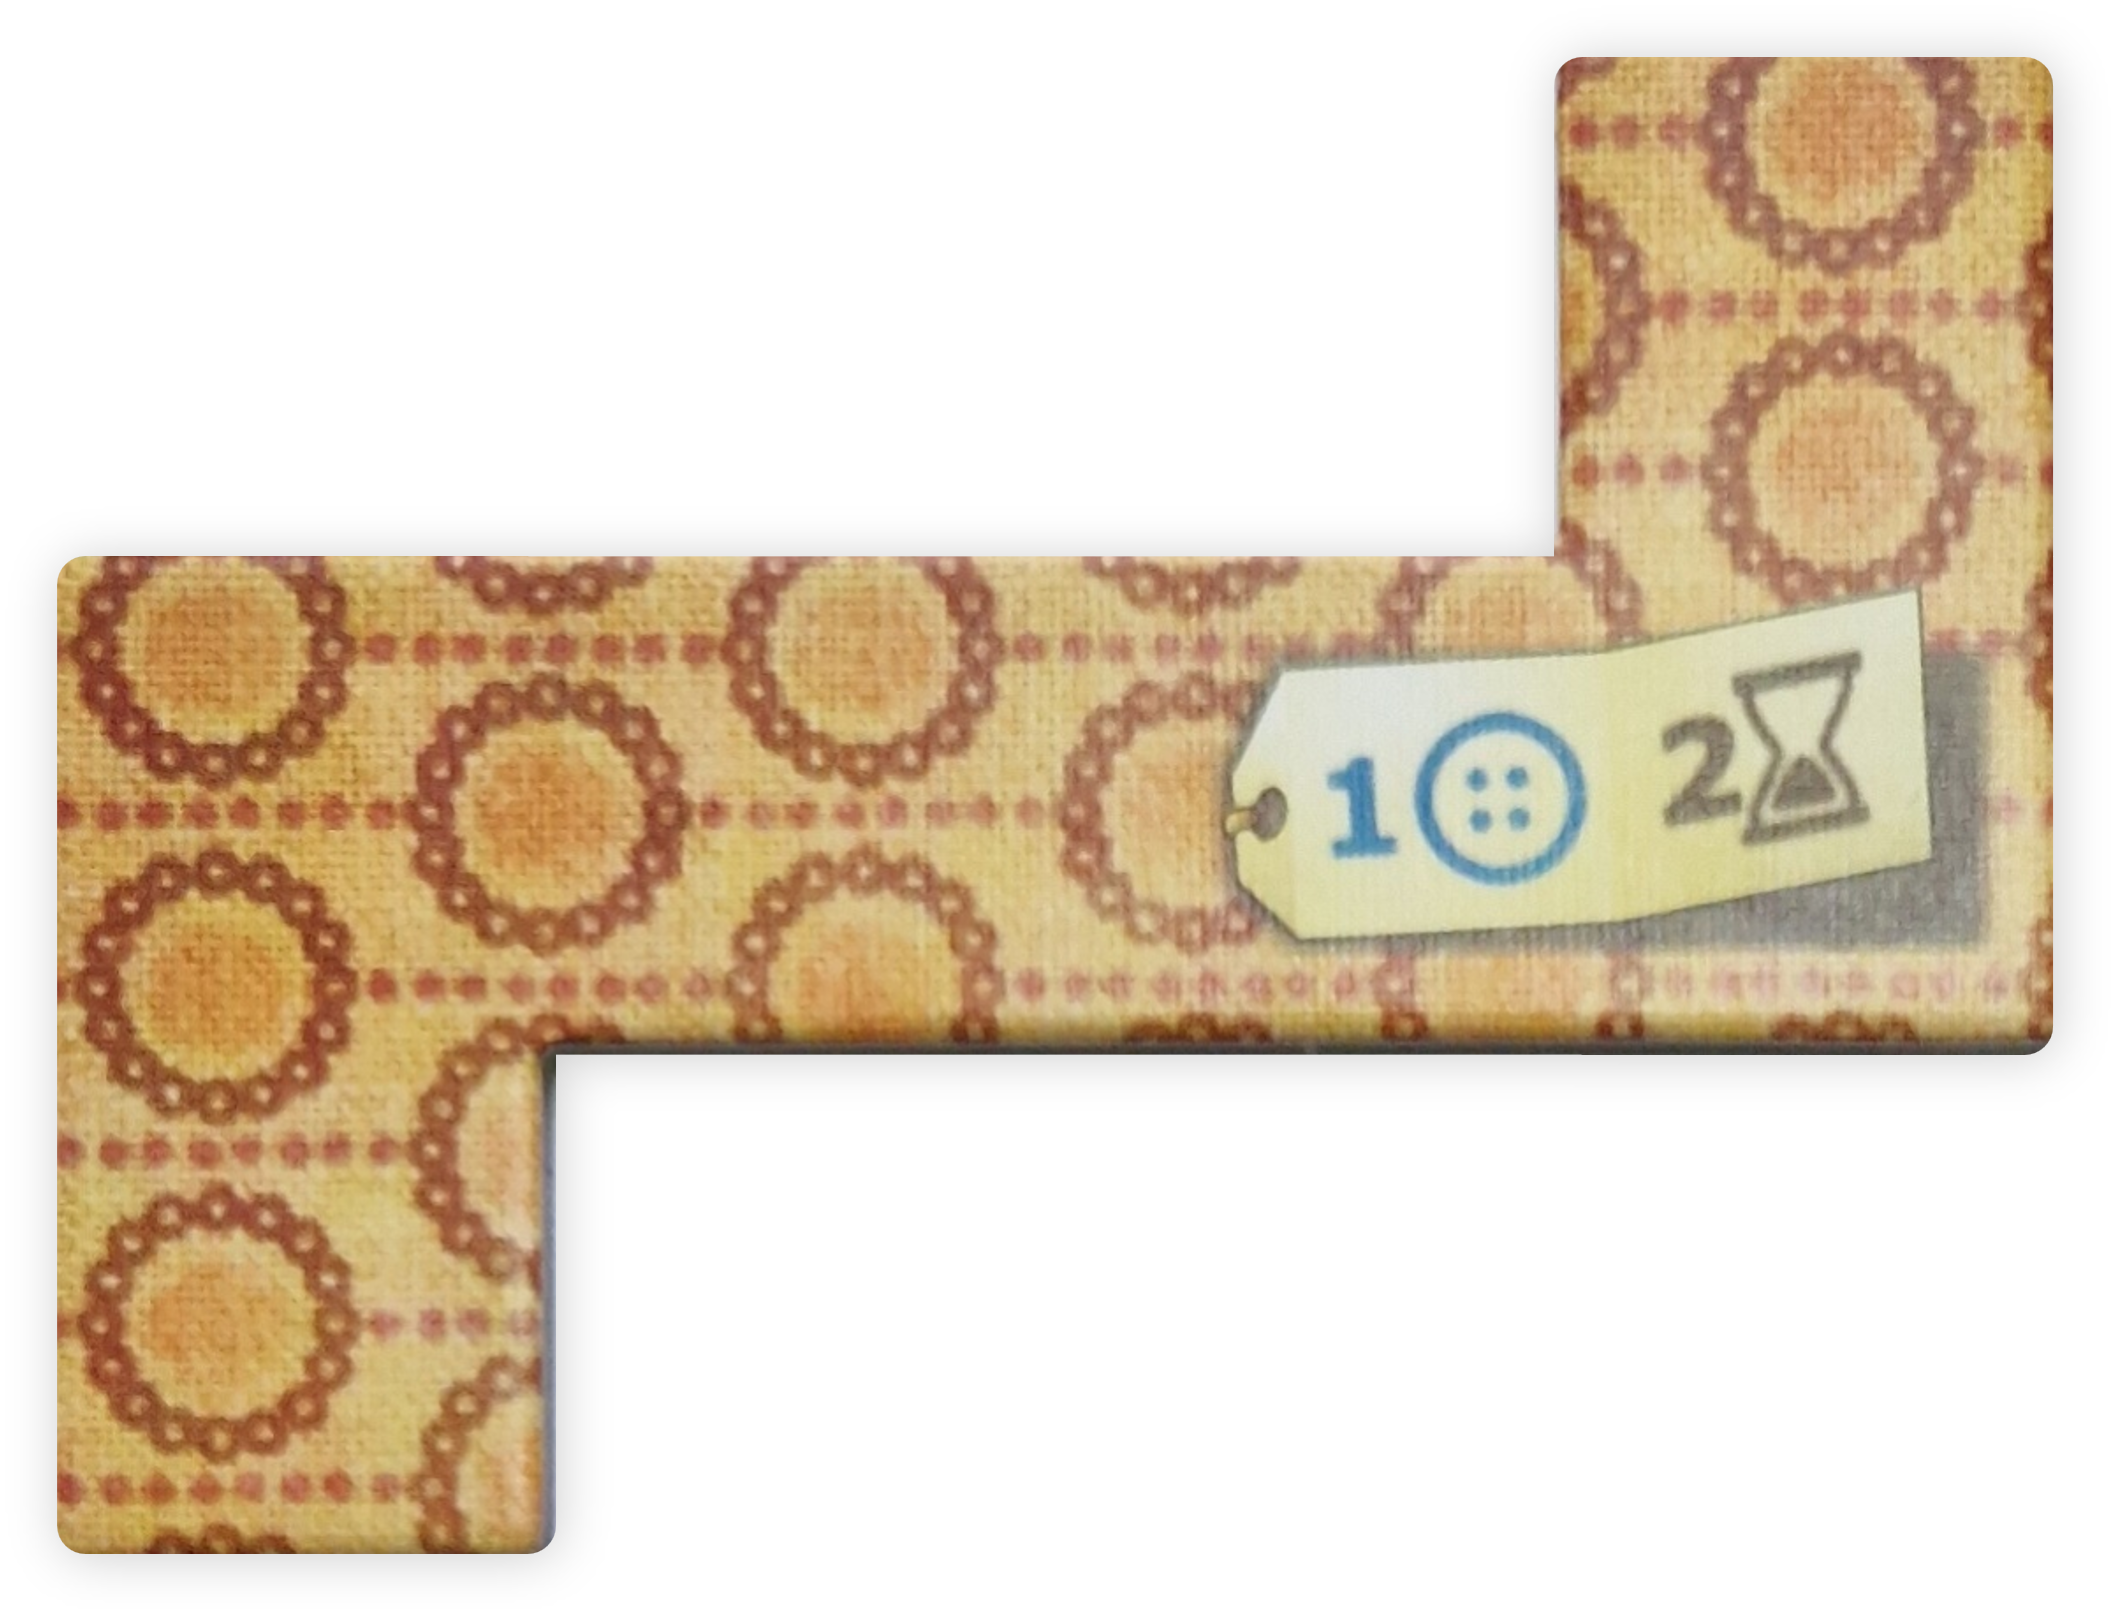
\includegraphics[width=0.2\textwidth]{res/pictures/assets/11-front.png}} & $11$ & $6$    & $1$              & $2$ & $0$ & $0$                            \\ \hline
    \adjustbox{valign=m, max width=0.2\textwidth, max height=0.1\textheight}{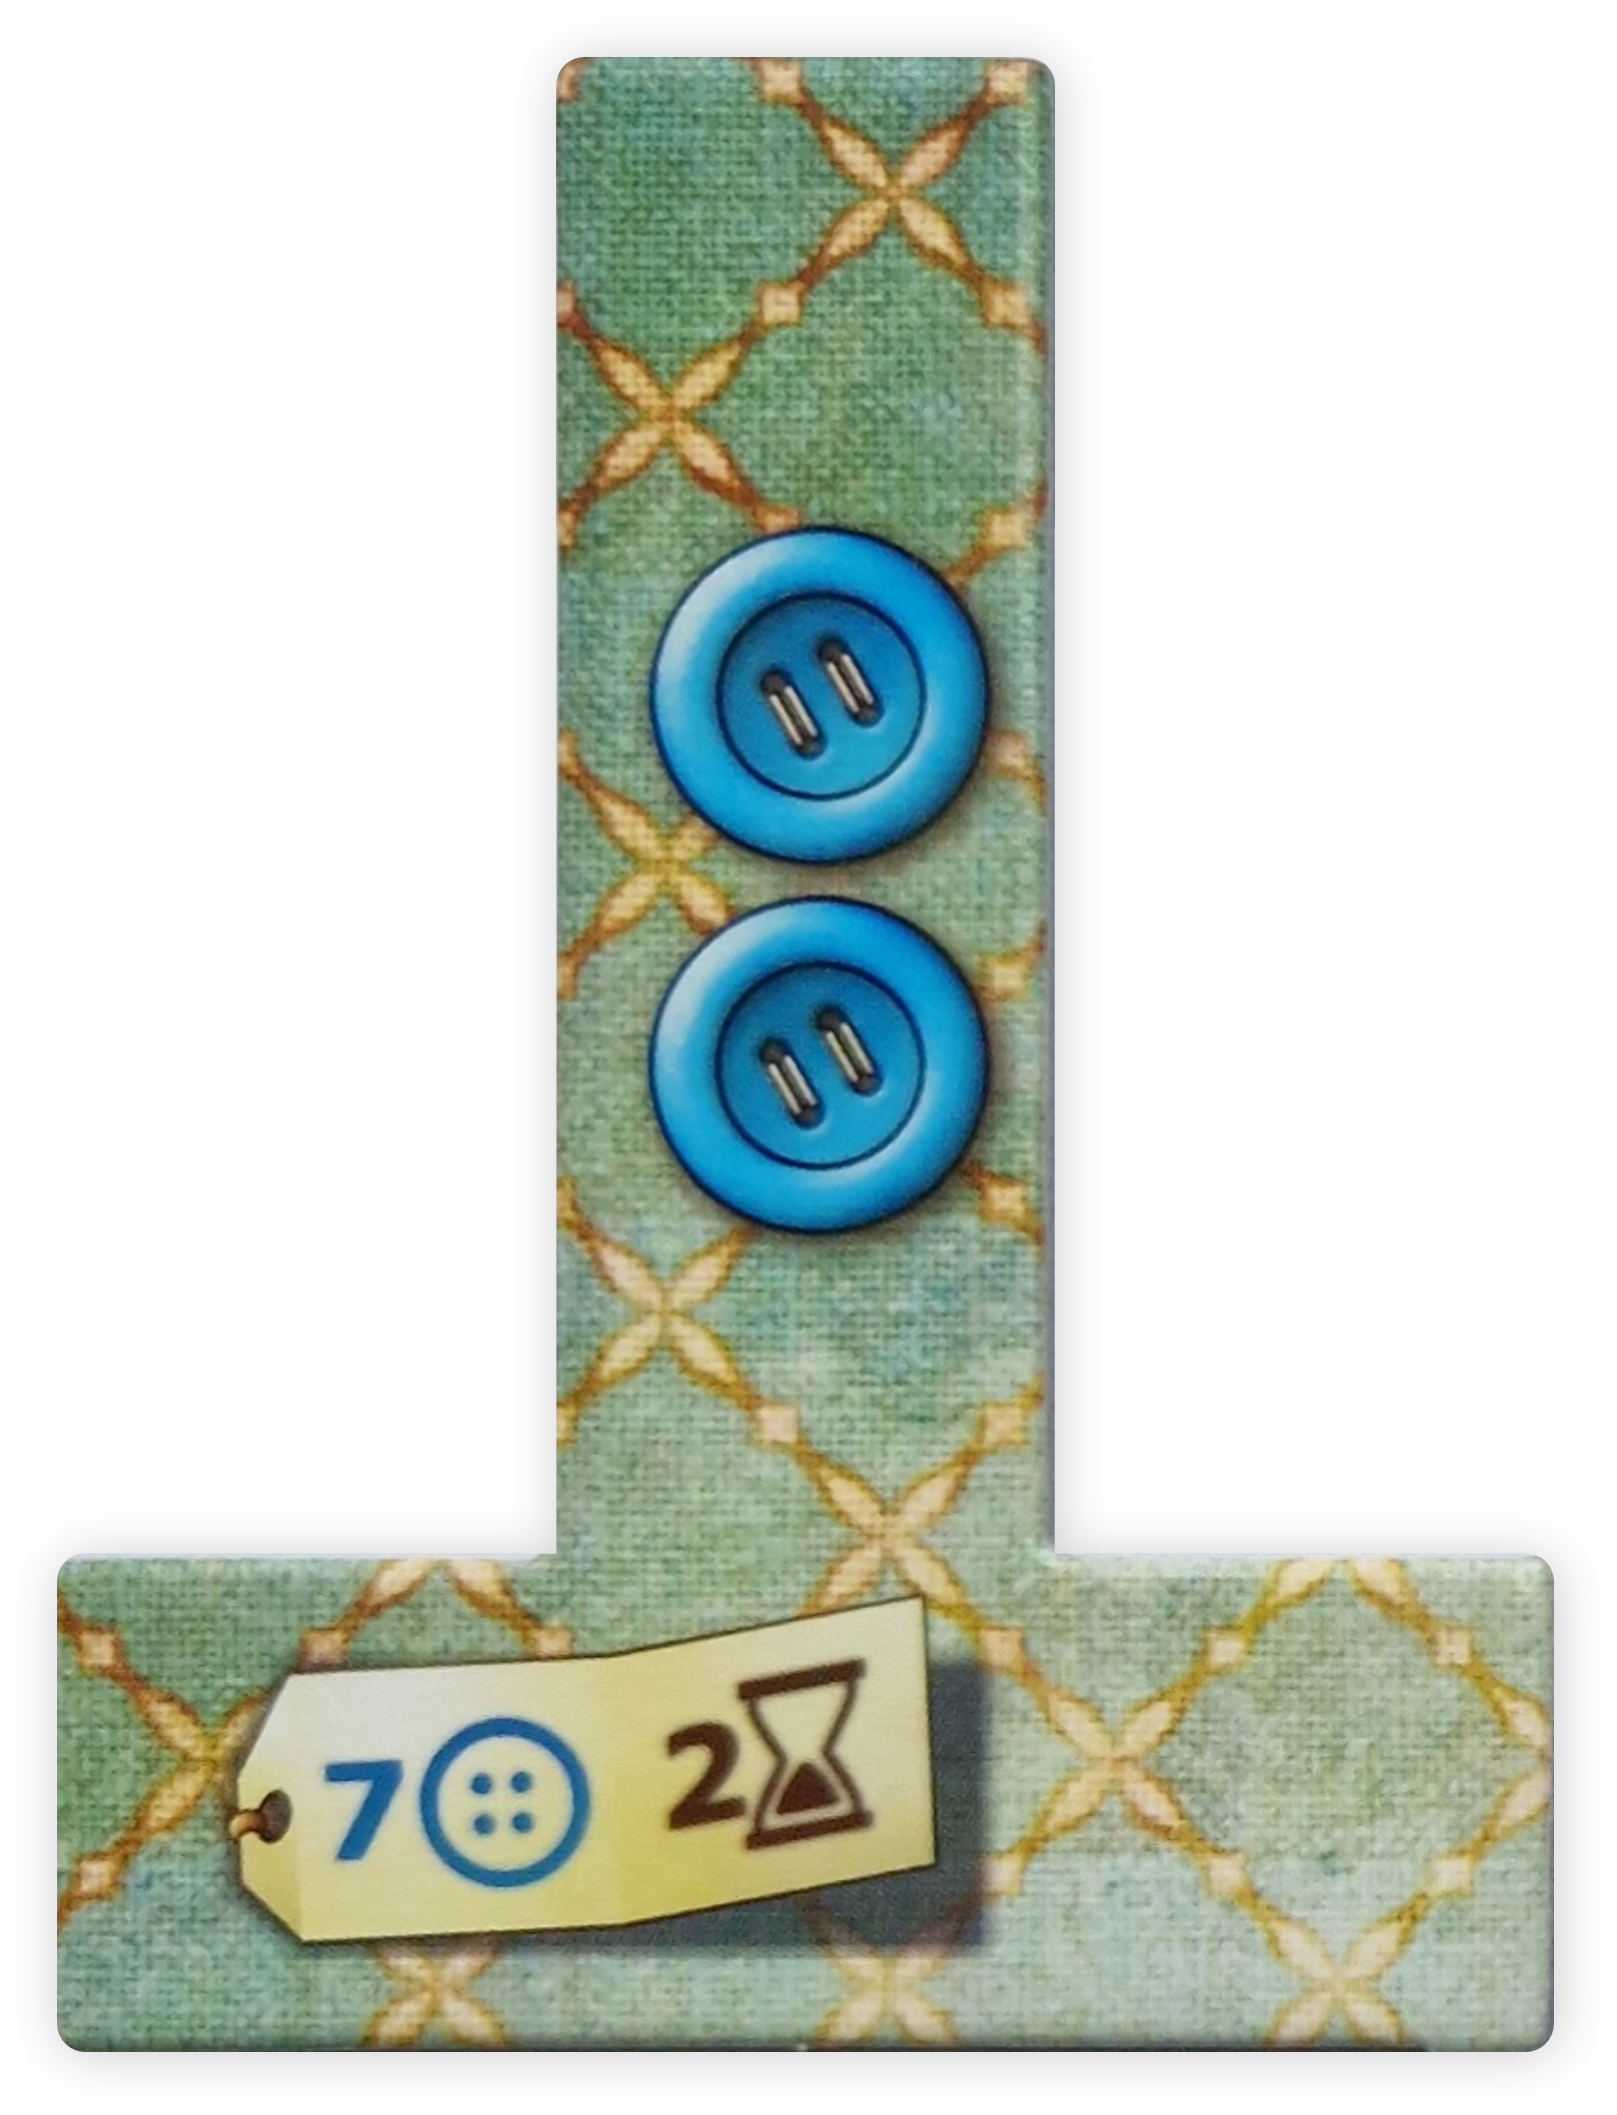
\includegraphics[width=0.2\textwidth]{res/pictures/assets/12-front.png}} & $12$ & $6$    & $10$             & $5$ & $3$ & $\frac{1}{10} = 0{,}1$         \\ \hline
    \adjustbox{valign=m, max width=0.2\textwidth, max height=0.1\textheight}{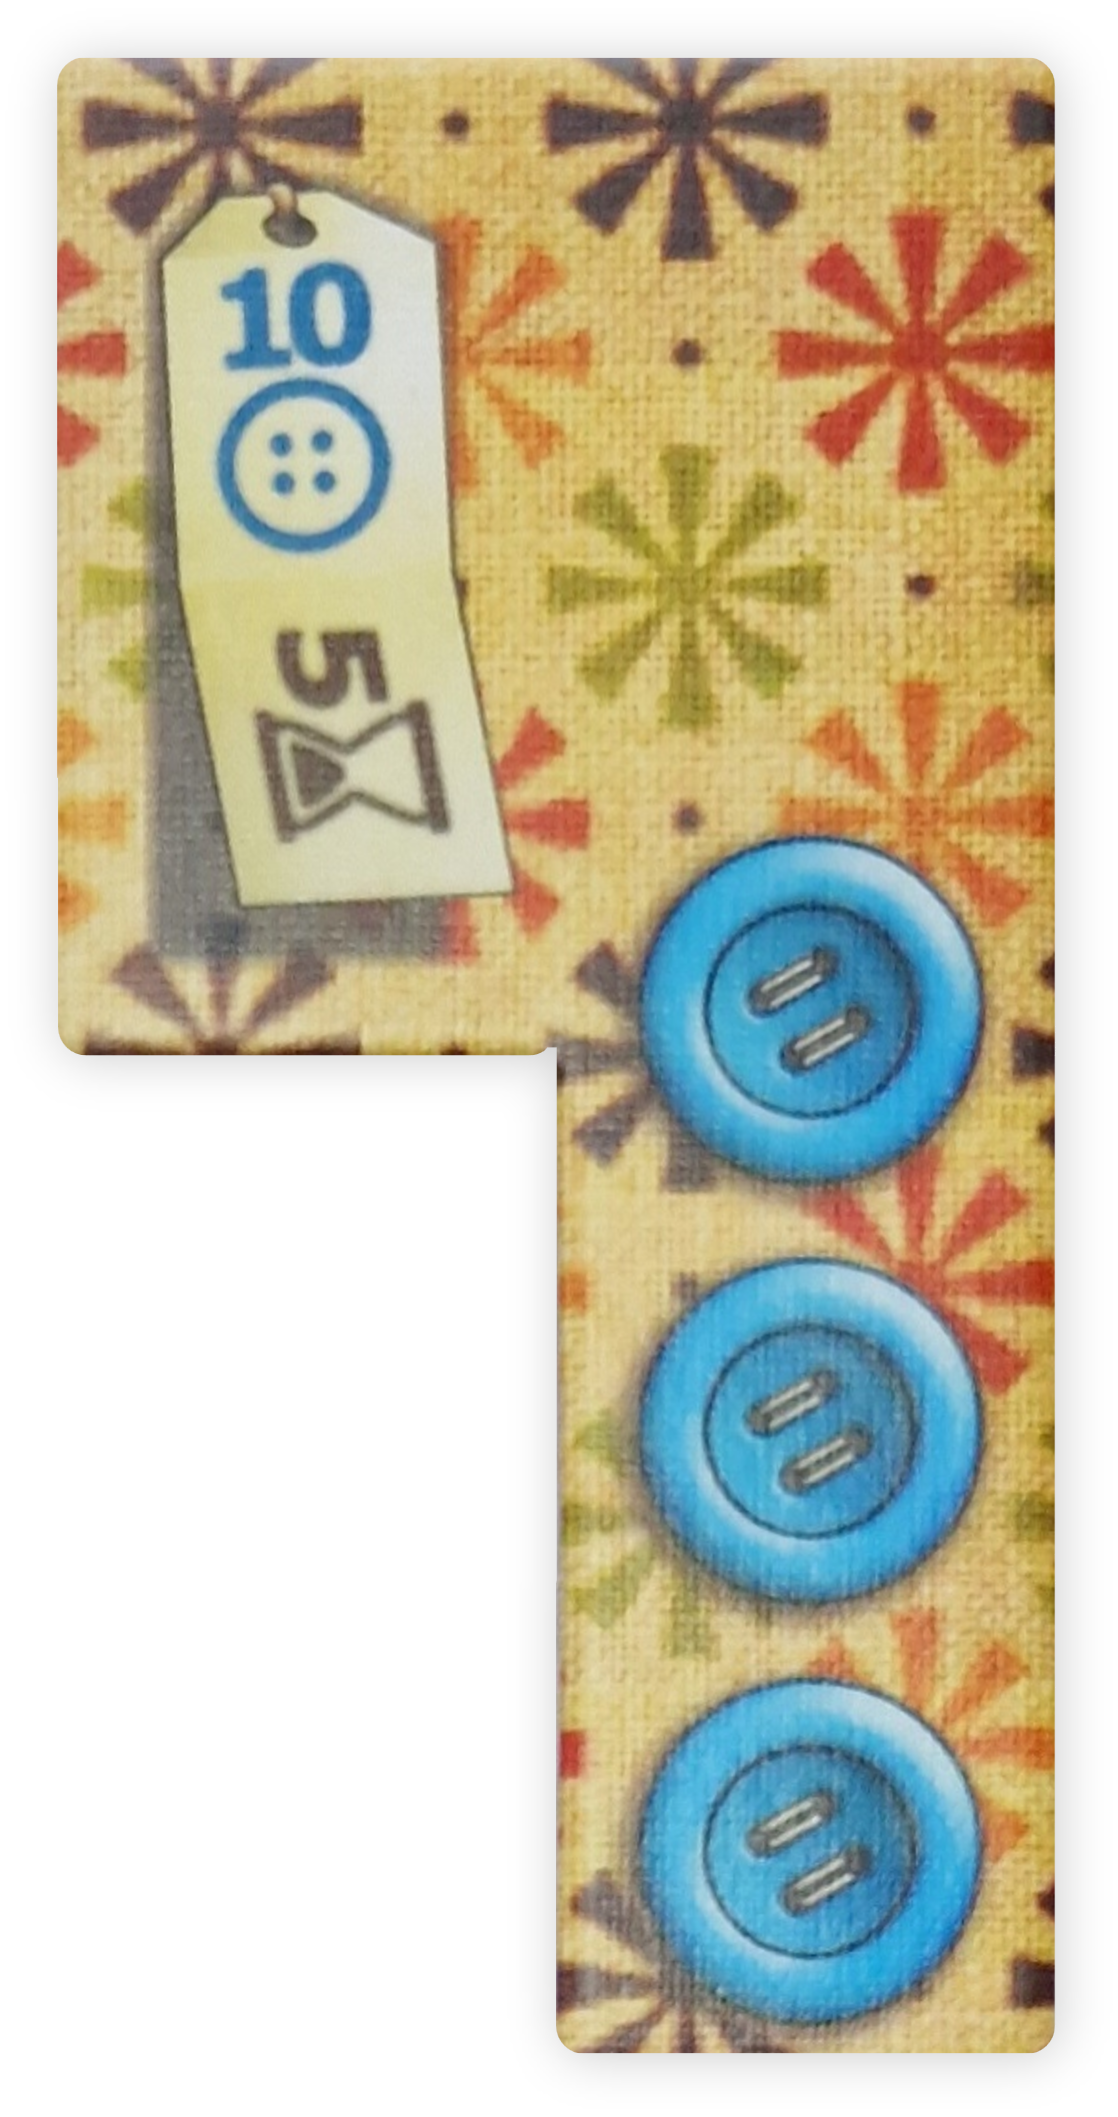
\includegraphics[width=0.2\textwidth]{res/pictures/assets/13-front.png}} & $13$ & $6$    & $7$              & $2$ & $2$ & $\frac{1}{16} \approx 0{,}167$ \\ \hline
    \adjustbox{valign=m, max width=0.2\textwidth, max height=0.1\textheight}{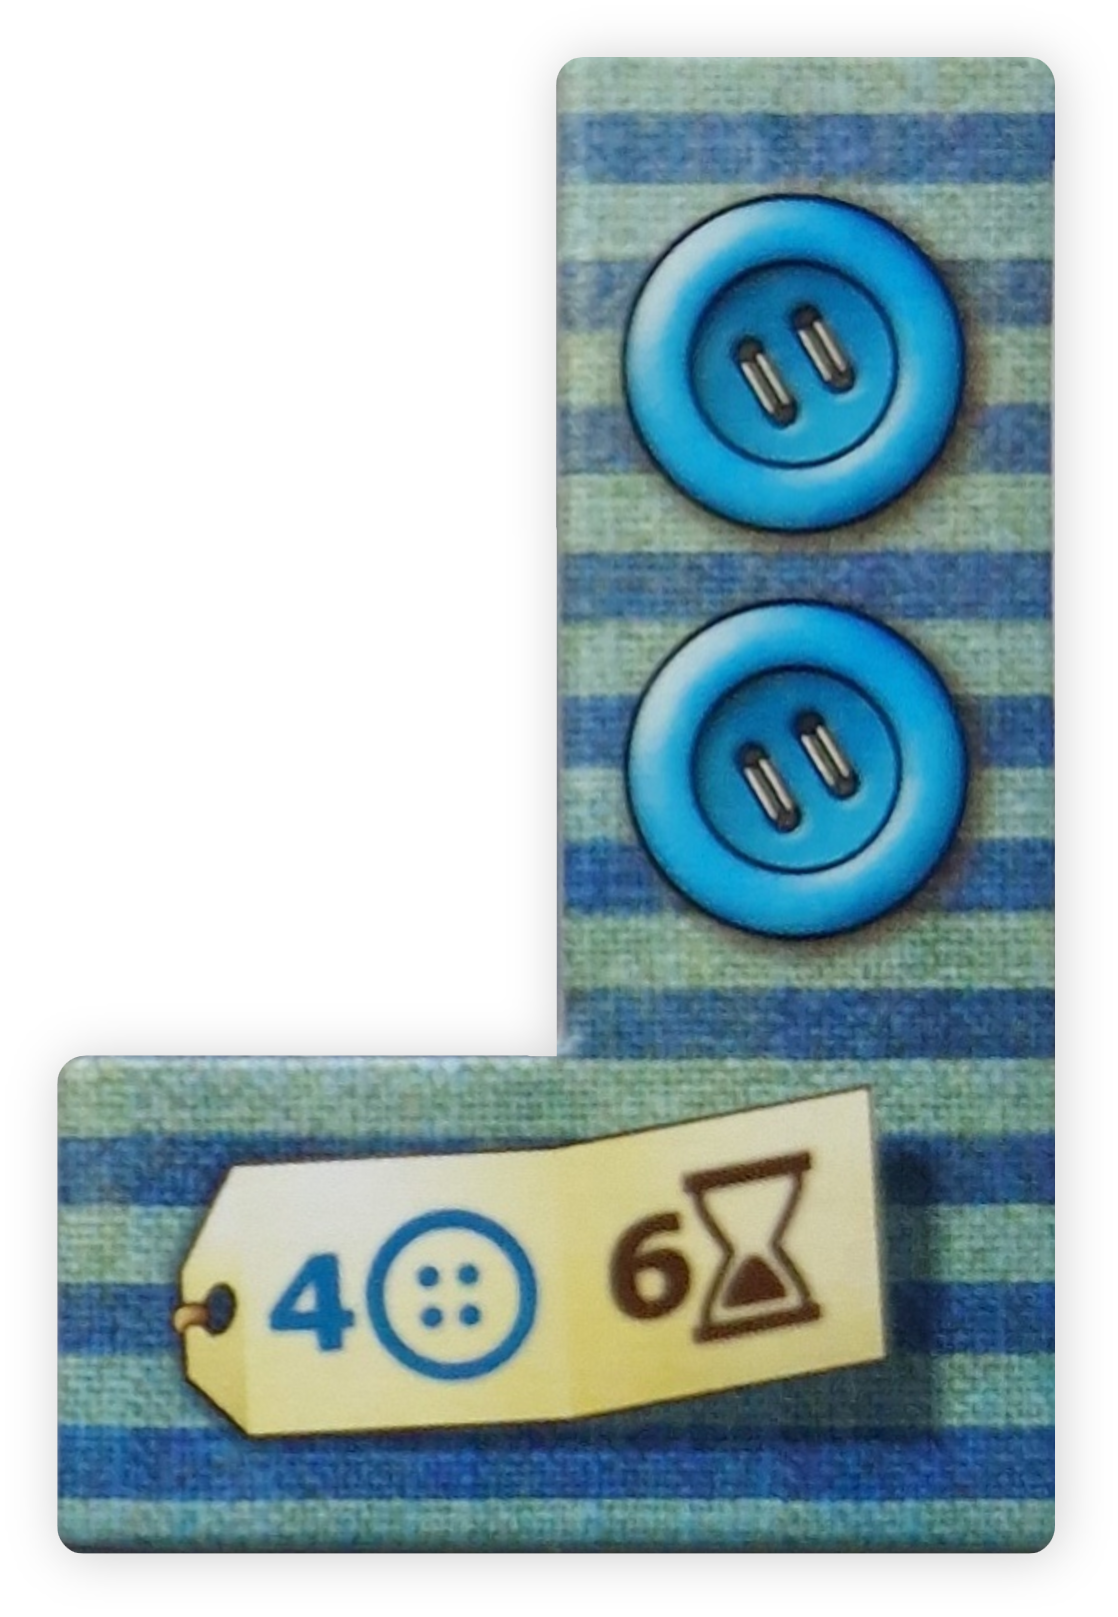
\includegraphics[width=0.2\textwidth]{res/pictures/assets/14-front.png}} & $14$ & $4$    & $4$              & $6$ & $2$ & $\frac{1}{12} \approx 0{,}083$ \\ \hline
    \adjustbox{valign=m, max width=0.2\textwidth, max height=0.1\textheight}{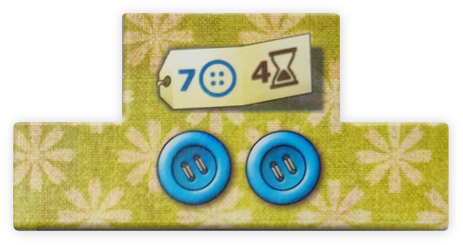
\includegraphics[width=0.2\textwidth]{res/pictures/assets/15-front.png}} & $15$ & $6$    & $7$              & $4$ & $2$ & $\frac{1}{12} \approx 0{,}083$ \\ \hline
    \adjustbox{valign=m, max width=0.2\textwidth, max height=0.1\textheight}{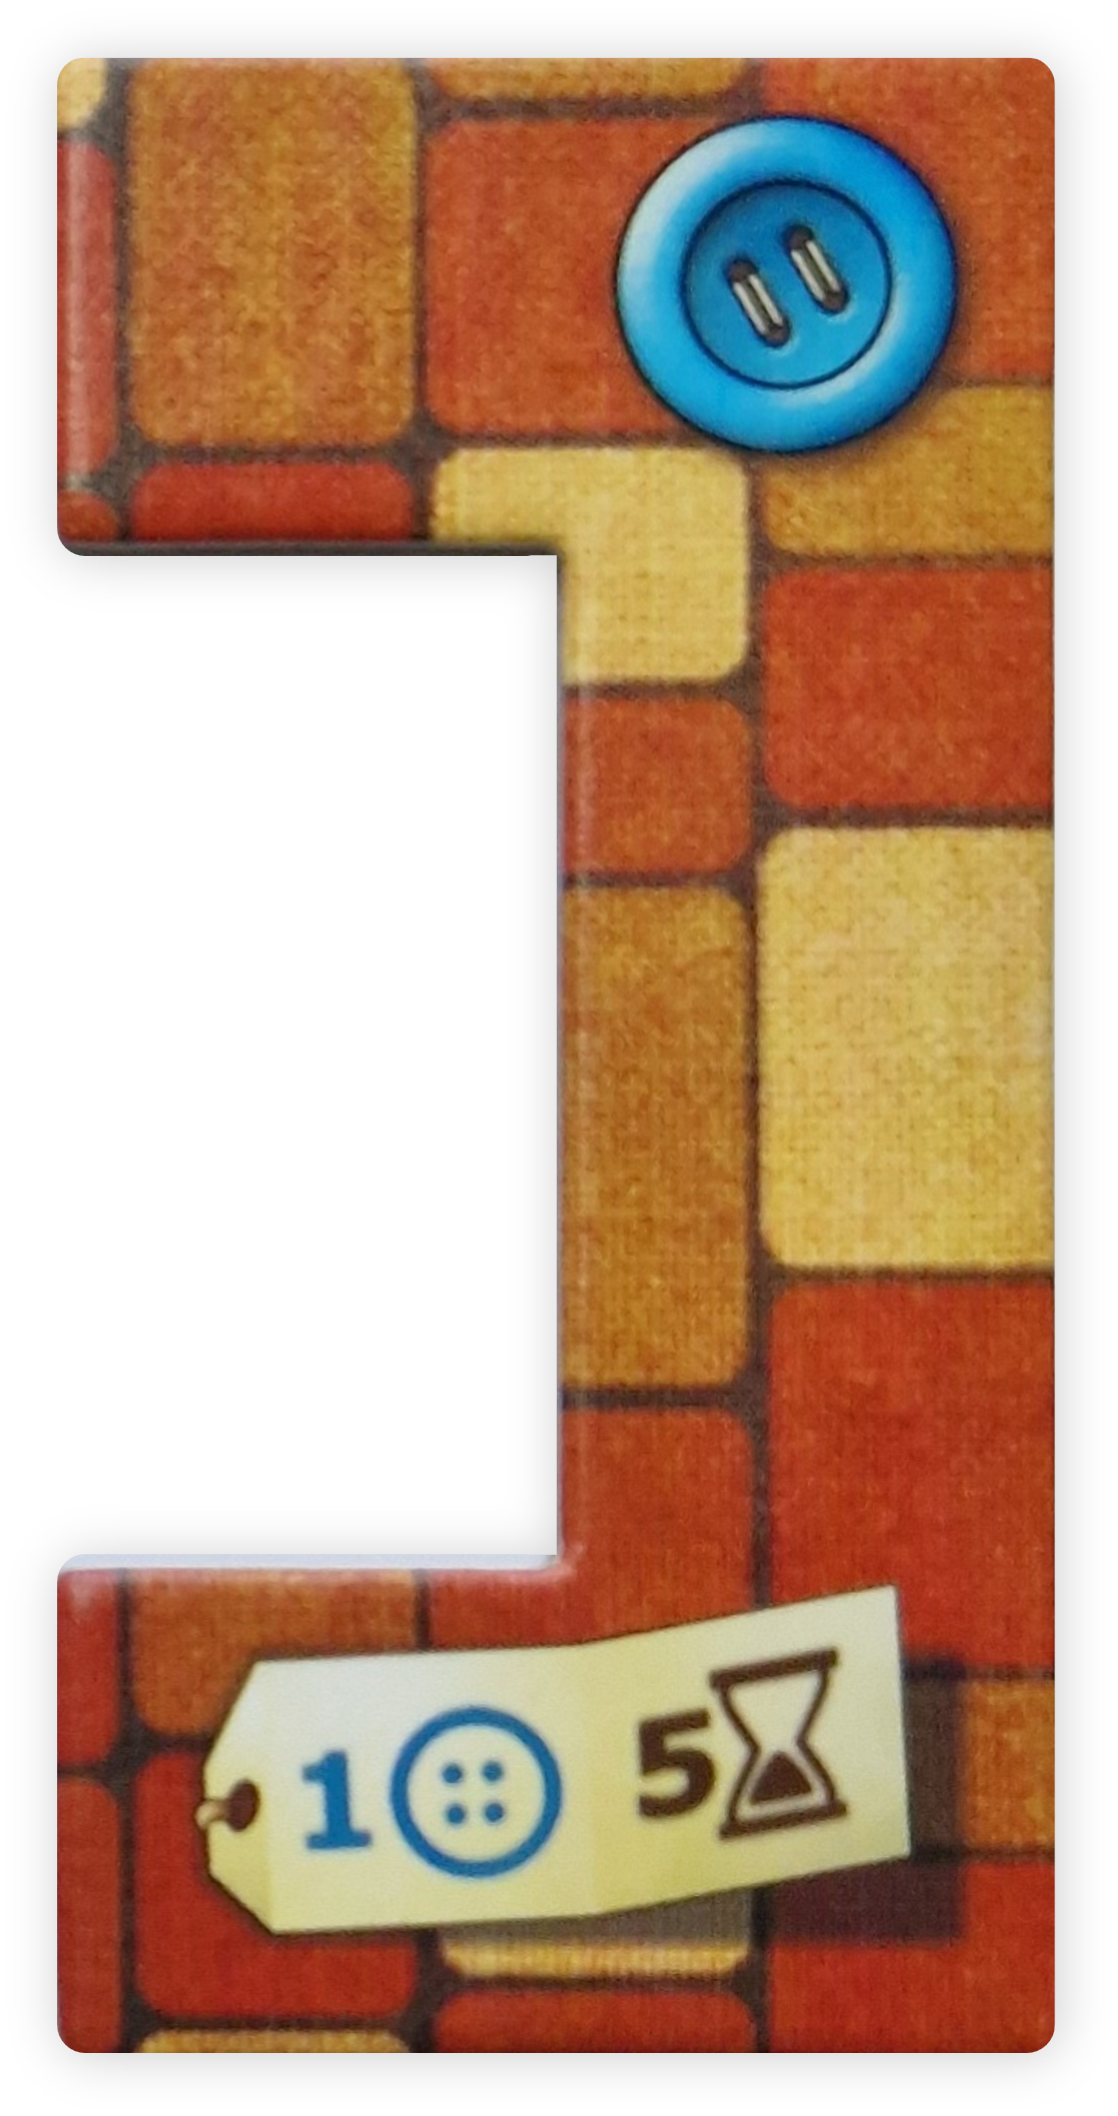
\includegraphics[width=0.2\textwidth]{res/pictures/assets/16-front.png}} & $16$ & $6$    & $1$              & $5$ & $1$ & $\frac{1}{30} \approx 0{,}033$ \\ \hline
    \adjustbox{valign=m, max width=0.2\textwidth, max height=0.1\textheight}{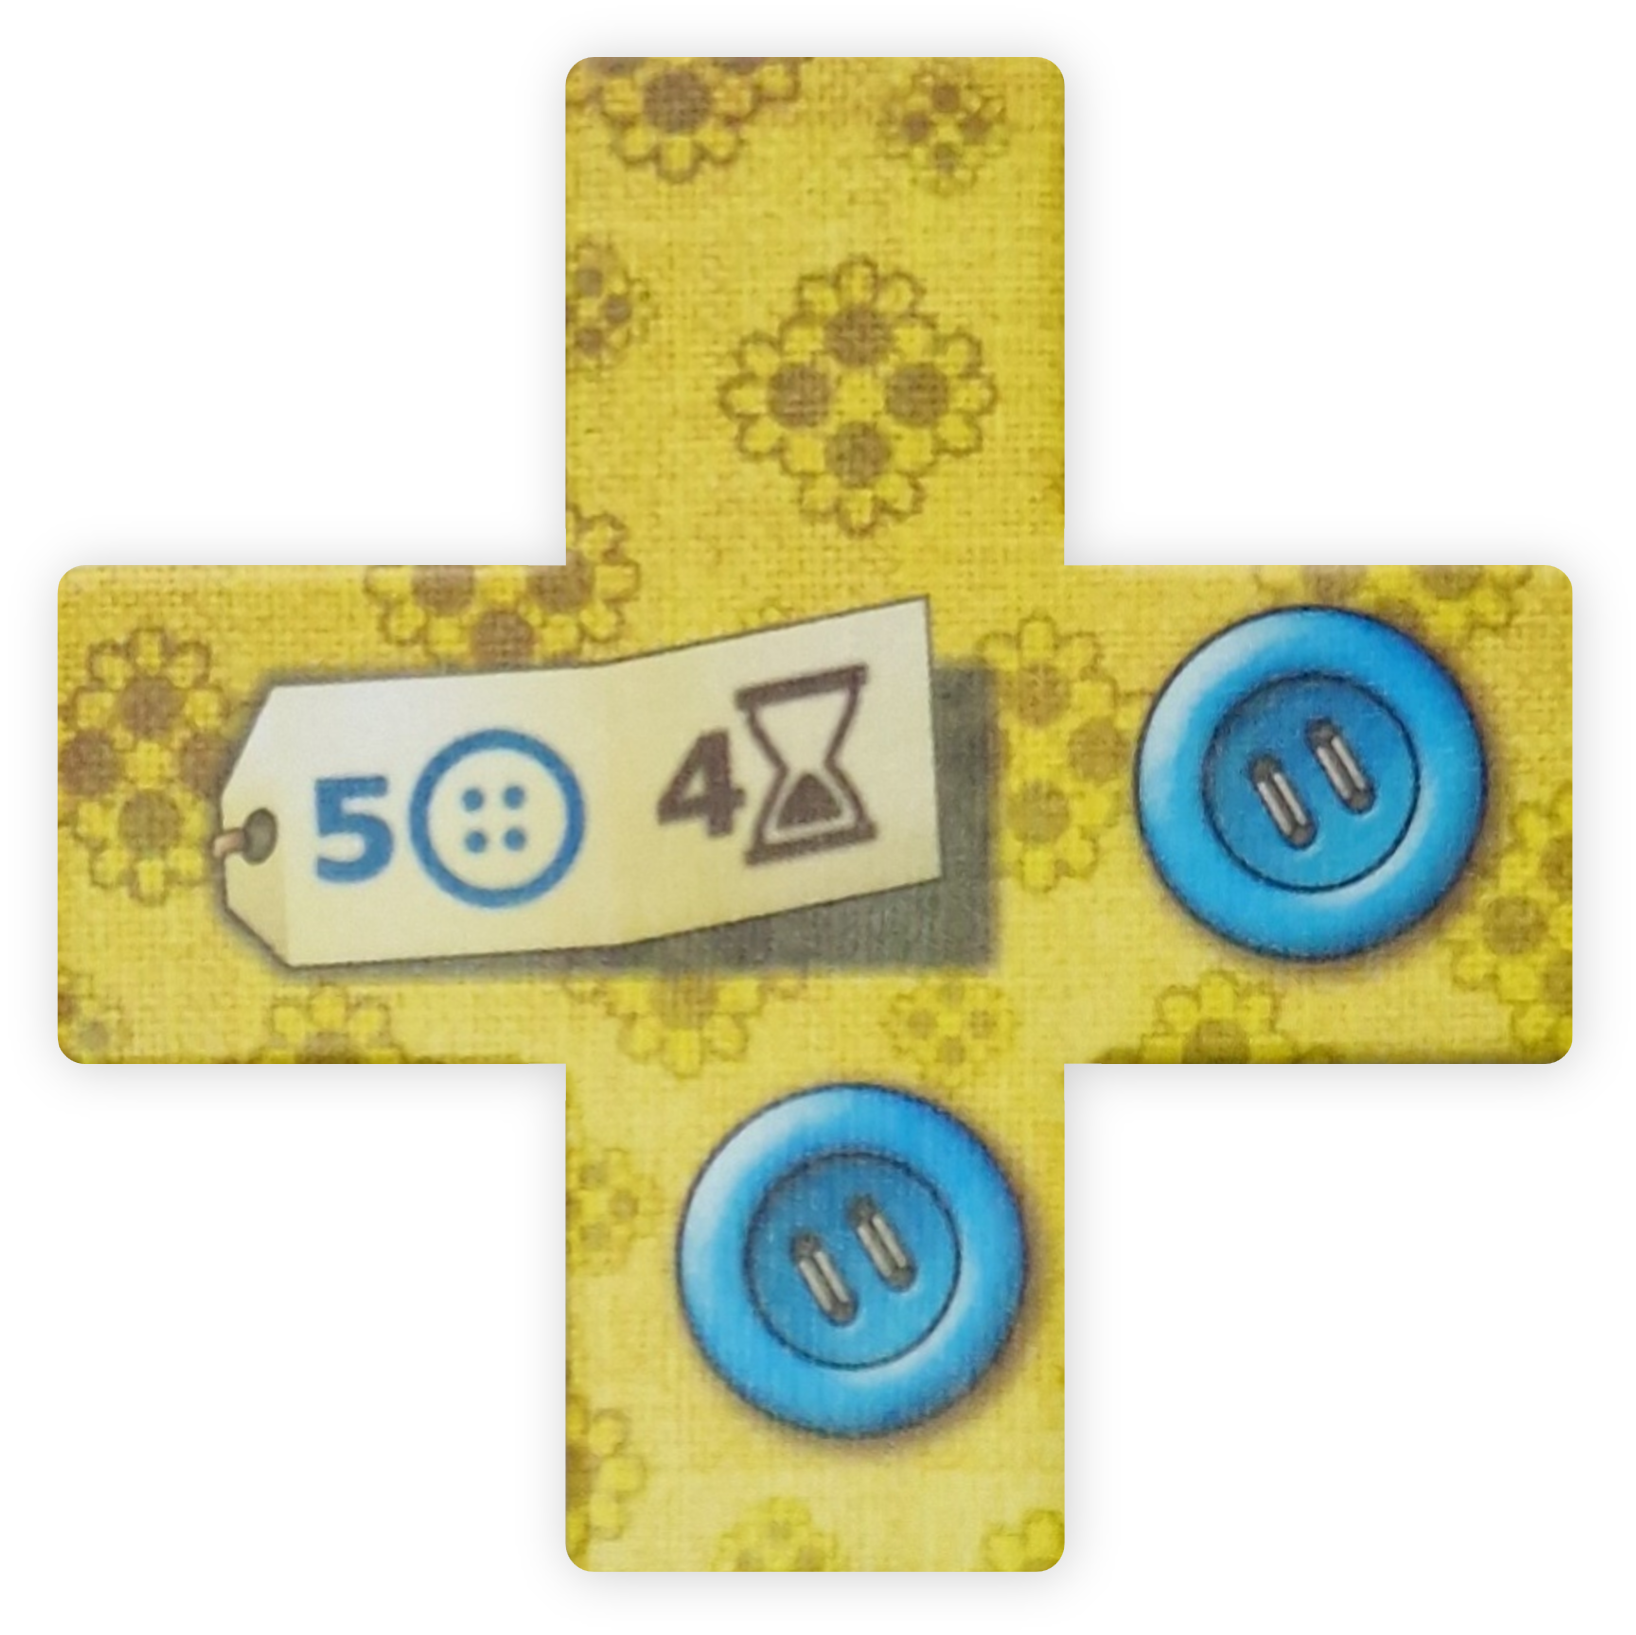
\includegraphics[width=0.2\textwidth]{res/pictures/assets/17-front.png}} & $17$ & $5$    & $5$              & $4$ & $2$ & $\frac{1}{10} = 0{,}1$         \\ \hline
    \adjustbox{valign=m, max width=0.2\textwidth, max height=0.1\textheight}{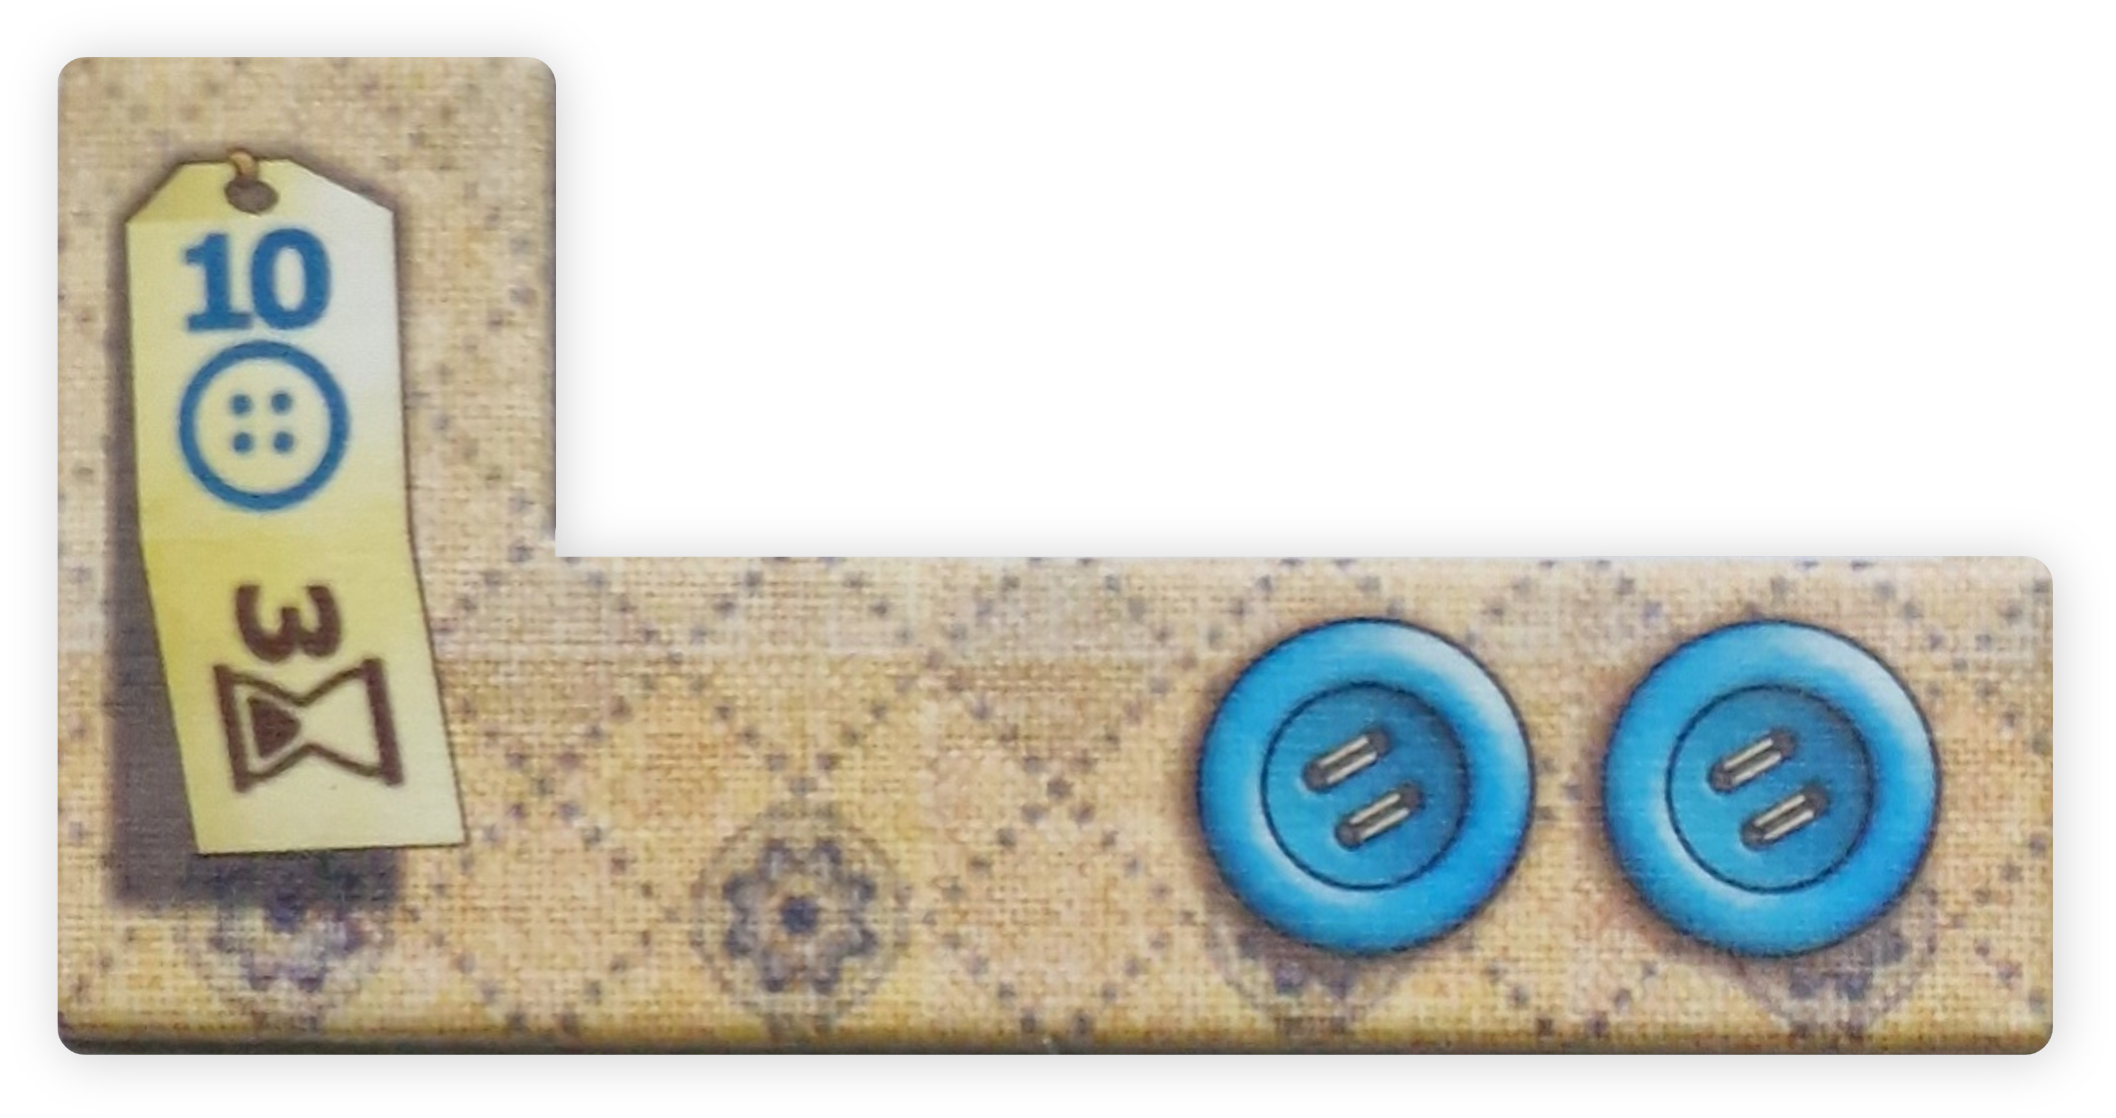
\includegraphics[width=0.2\textwidth]{res/pictures/assets/18-front.png}} & $18$ & $5$    & $10$             & $3$ & $2$ & $\frac{2}{15} \approx 0{,}133$ \\ \hline
    \adjustbox{valign=m, max width=0.2\textwidth, max height=0.1\textheight}{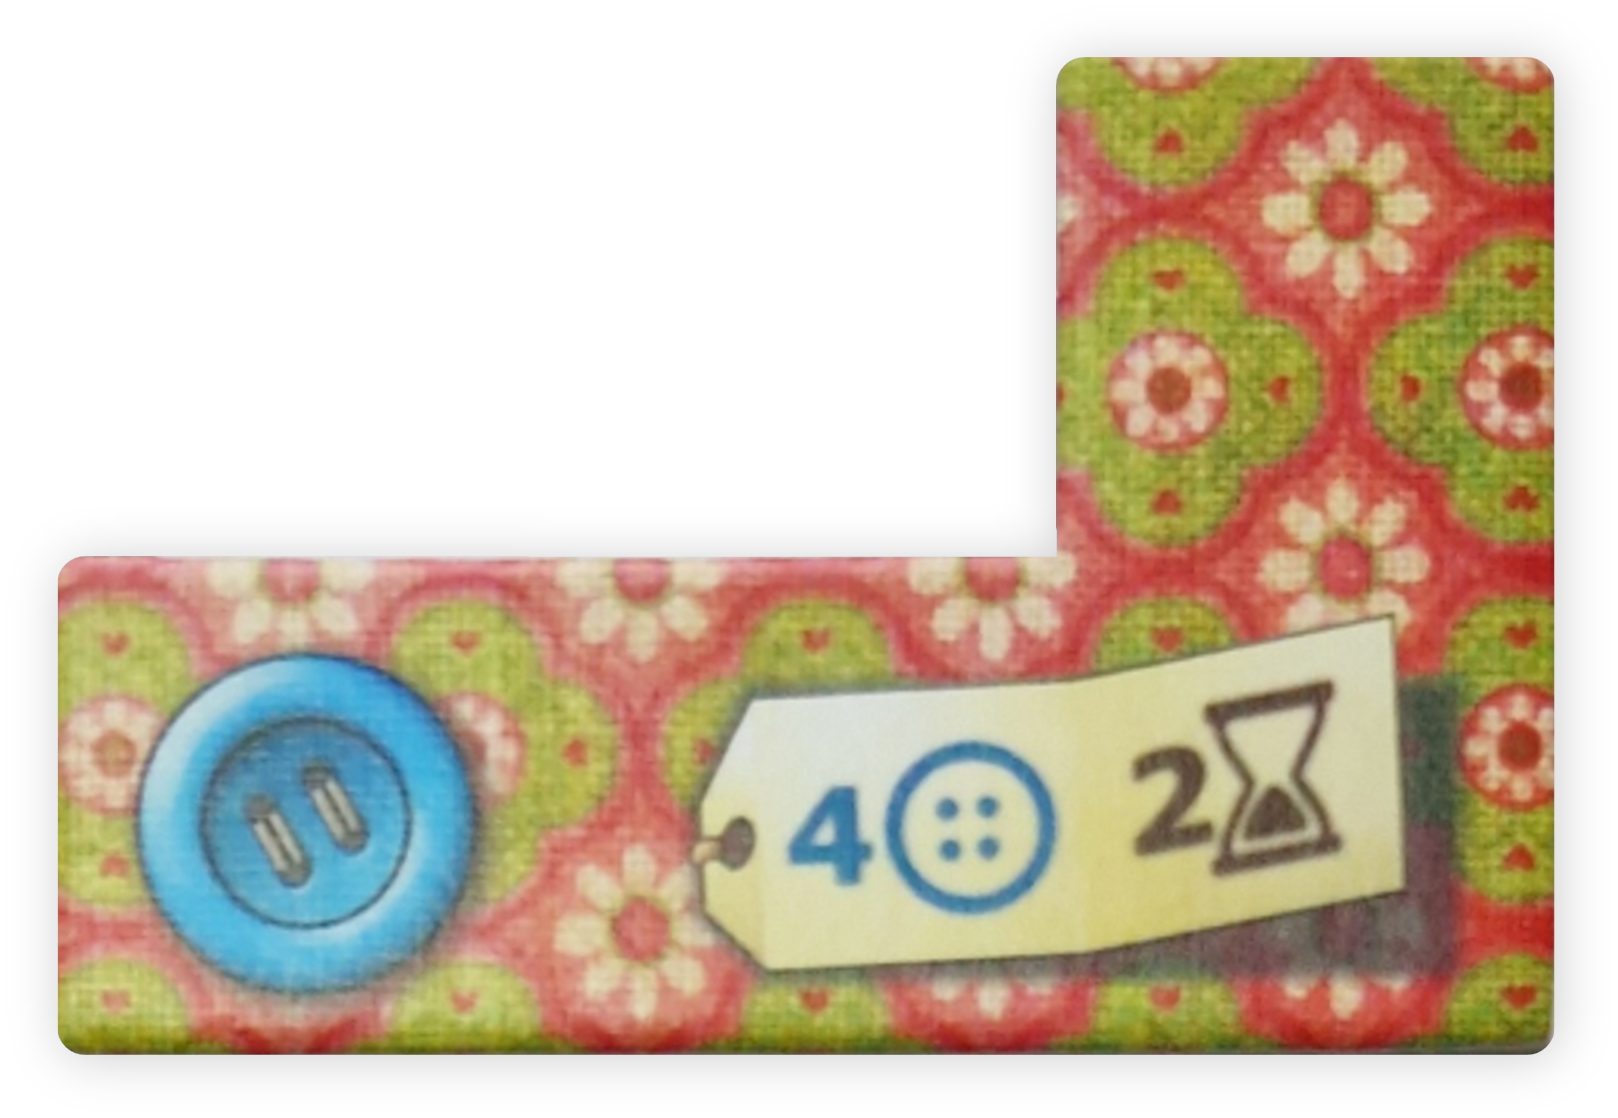
\includegraphics[width=0.2\textwidth]{res/pictures/assets/19-front.png}} & $19$ & $4$    & $4$              & $2$ & $1$ & $\frac{1}{8} = 0{,}125$        \\ \hline
    \adjustbox{valign=m, max width=0.2\textwidth, max height=0.1\textheight}{\includegraphics[width=0.2\textwidth]{res/pictures/assets/20-front.png}} & $20$ & $7$    & $1$              & $4$ & $1$ & $\frac{1}{28} \approx 0{,}036$ \\ \hline
    \adjustbox{valign=m, max width=0.2\textwidth, max height=0.1\textheight}{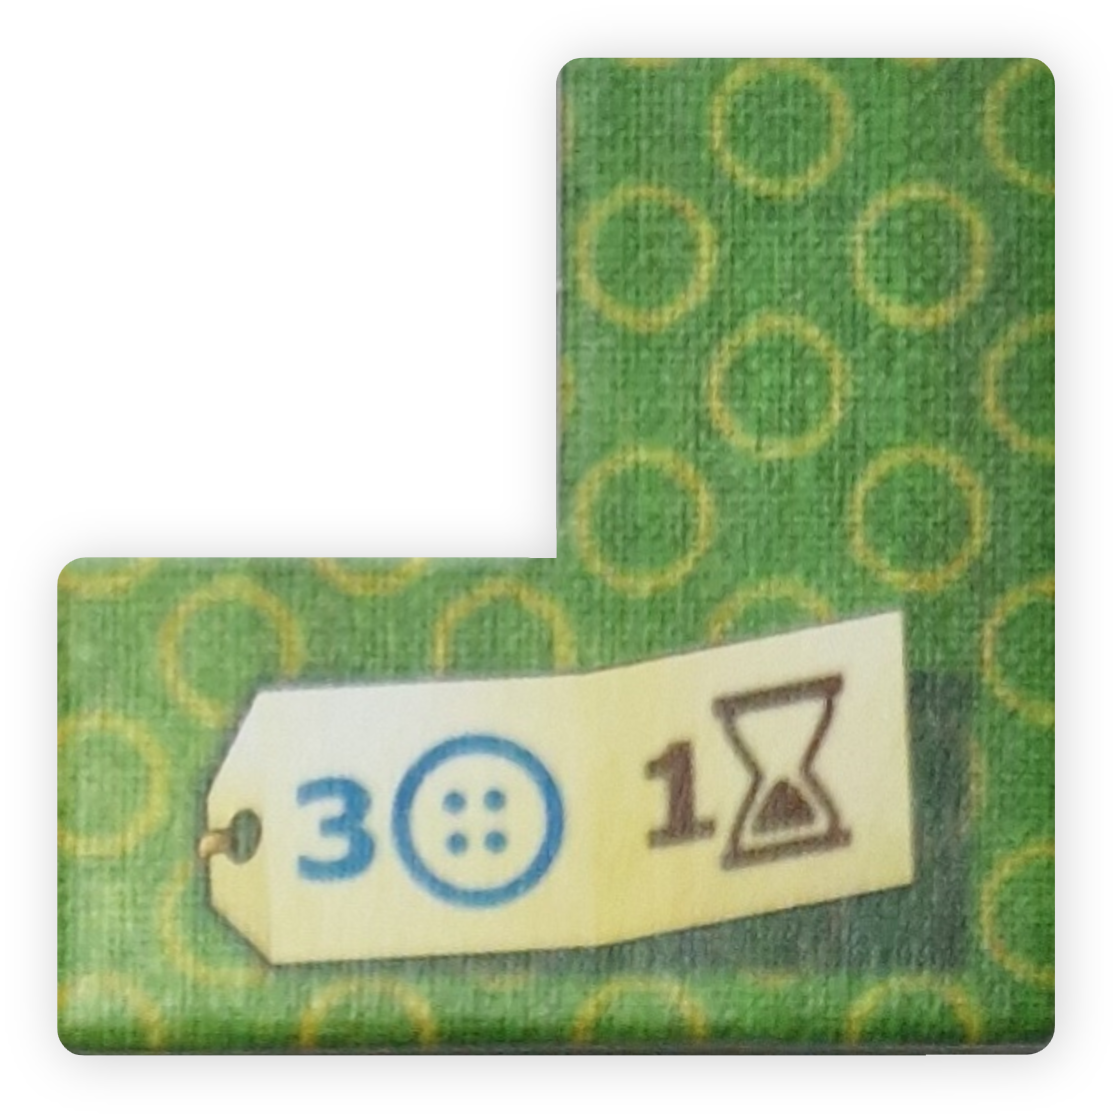
\includegraphics[width=0.2\textwidth]{res/pictures/assets/21-front.png}} & $21$ & $3$    & $1$              & $3$ & $0$ & $0$                            \\ \hline
    \adjustbox{valign=m, max width=0.2\textwidth, max height=0.1\textheight}{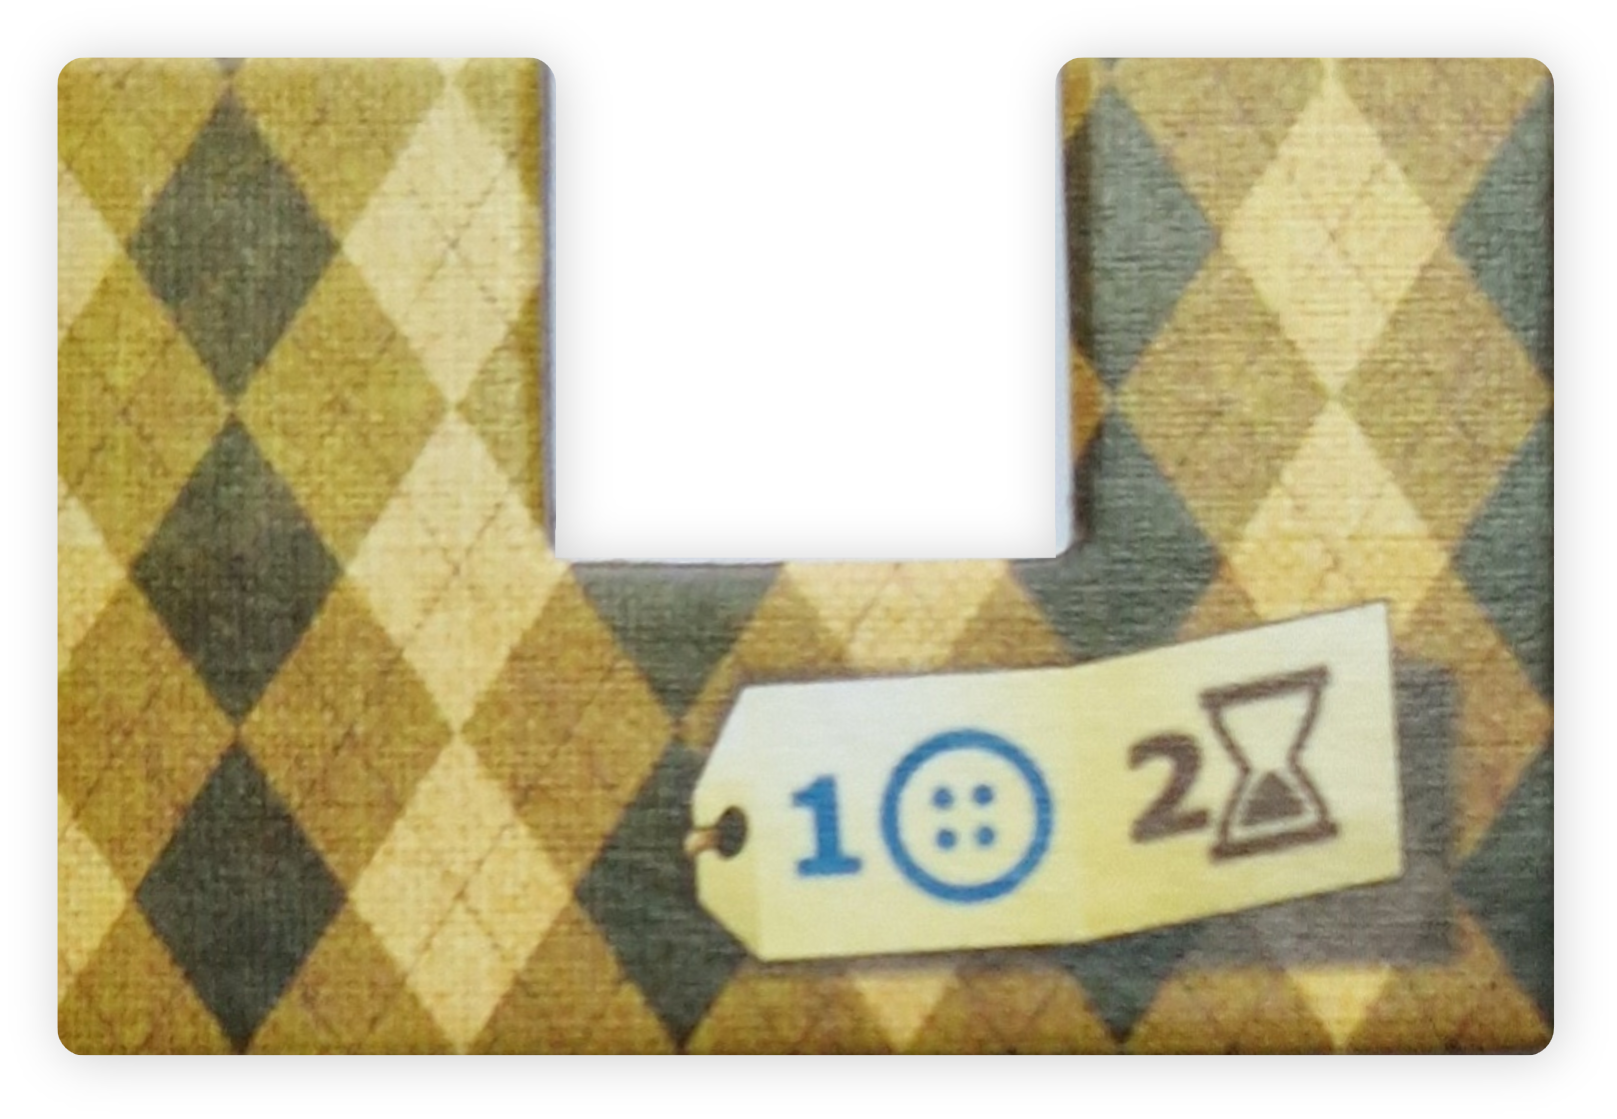
\includegraphics[width=0.2\textwidth]{res/pictures/assets/22-front.png}} & $22$ & $5$    & $1$              & $2$ & $0$ & $0$                            \\ \hline
    \adjustbox{valign=m, max width=0.2\textwidth, max height=0.1\textheight}{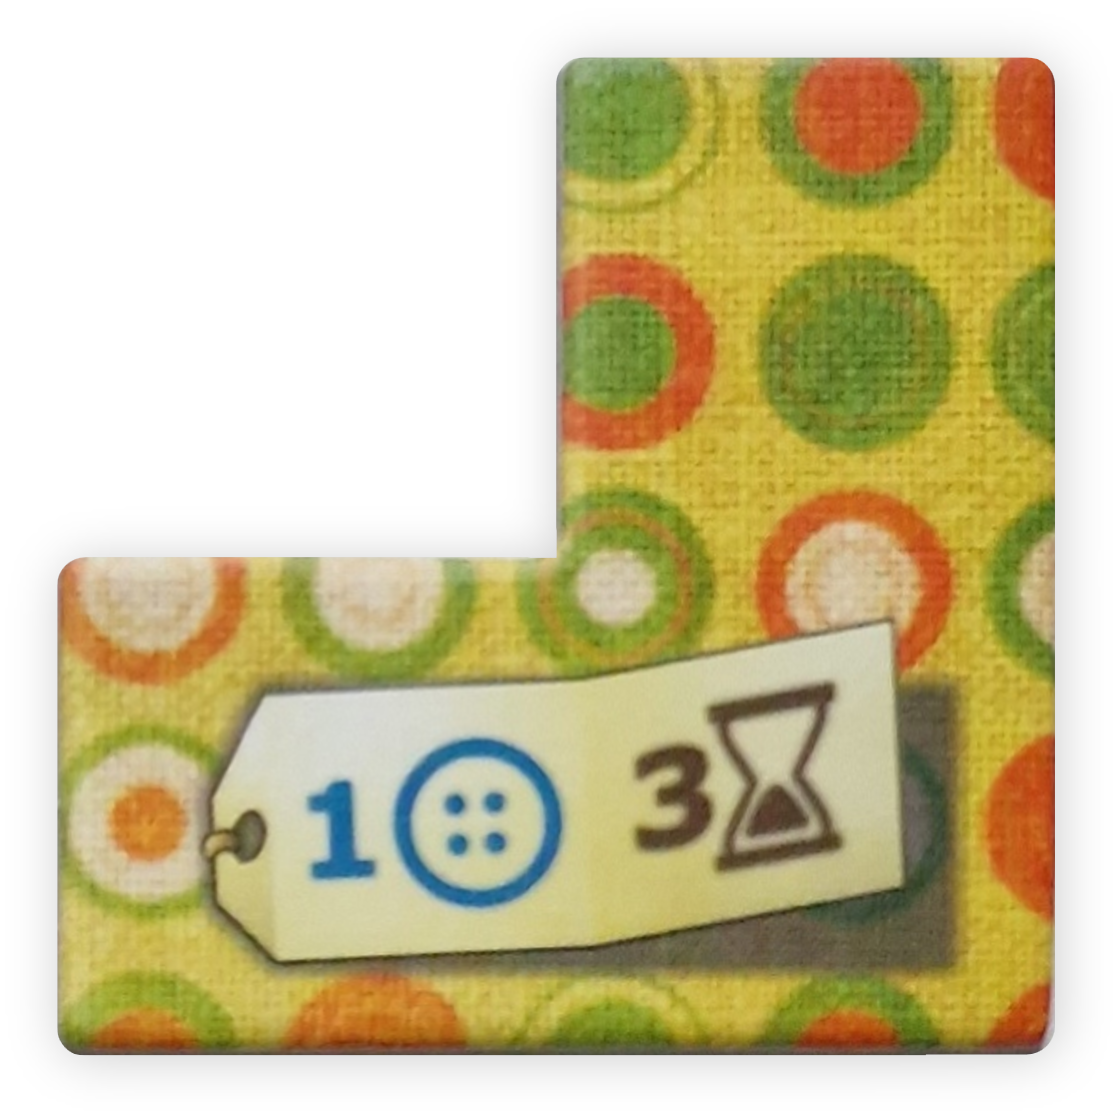
\includegraphics[width=0.2\textwidth]{res/pictures/assets/23-front.png}} & $23$ & $3$    & $3$              & $1$ & $0$ & $0$                            \\ \hline
    \adjustbox{valign=m, max width=0.2\textwidth, max height=0.1\textheight}{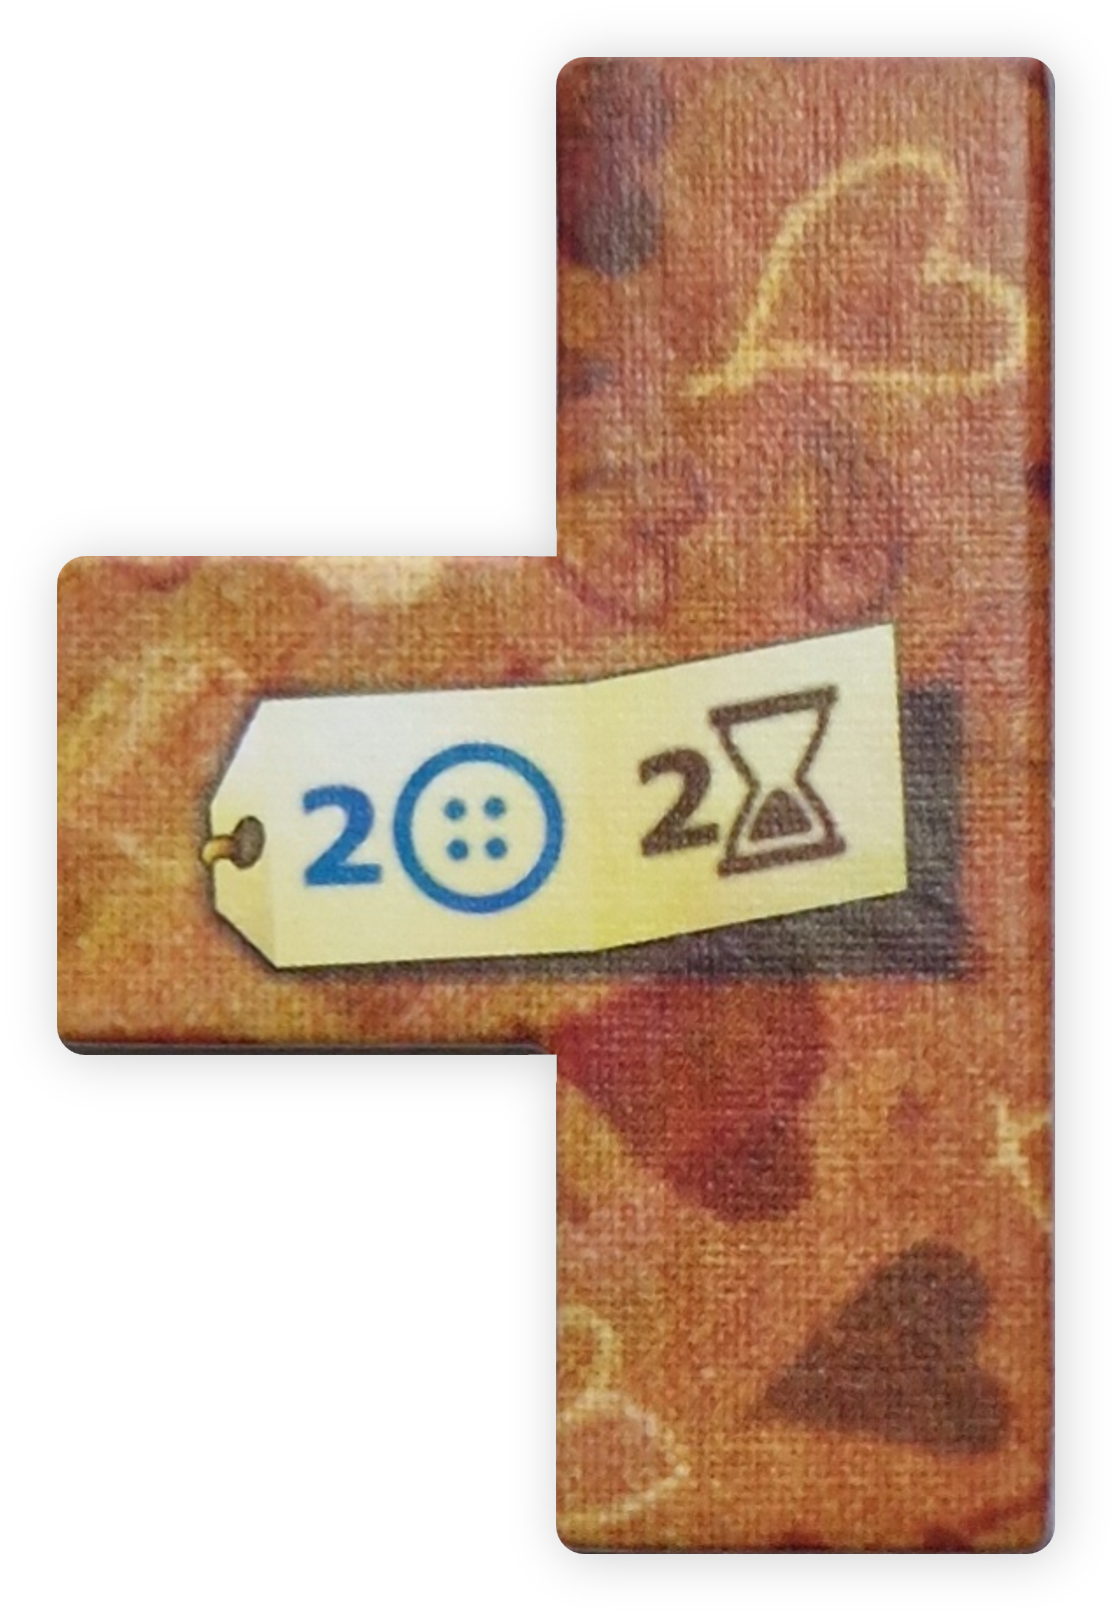
\includegraphics[width=0.2\textwidth]{res/pictures/assets/24-front.png}} & $24$ & $4$    & $2$              & $2$ & $0$ & $0$                            \\ \hline
    \adjustbox{valign=m, max width=0.2\textwidth, max height=0.1\textheight}{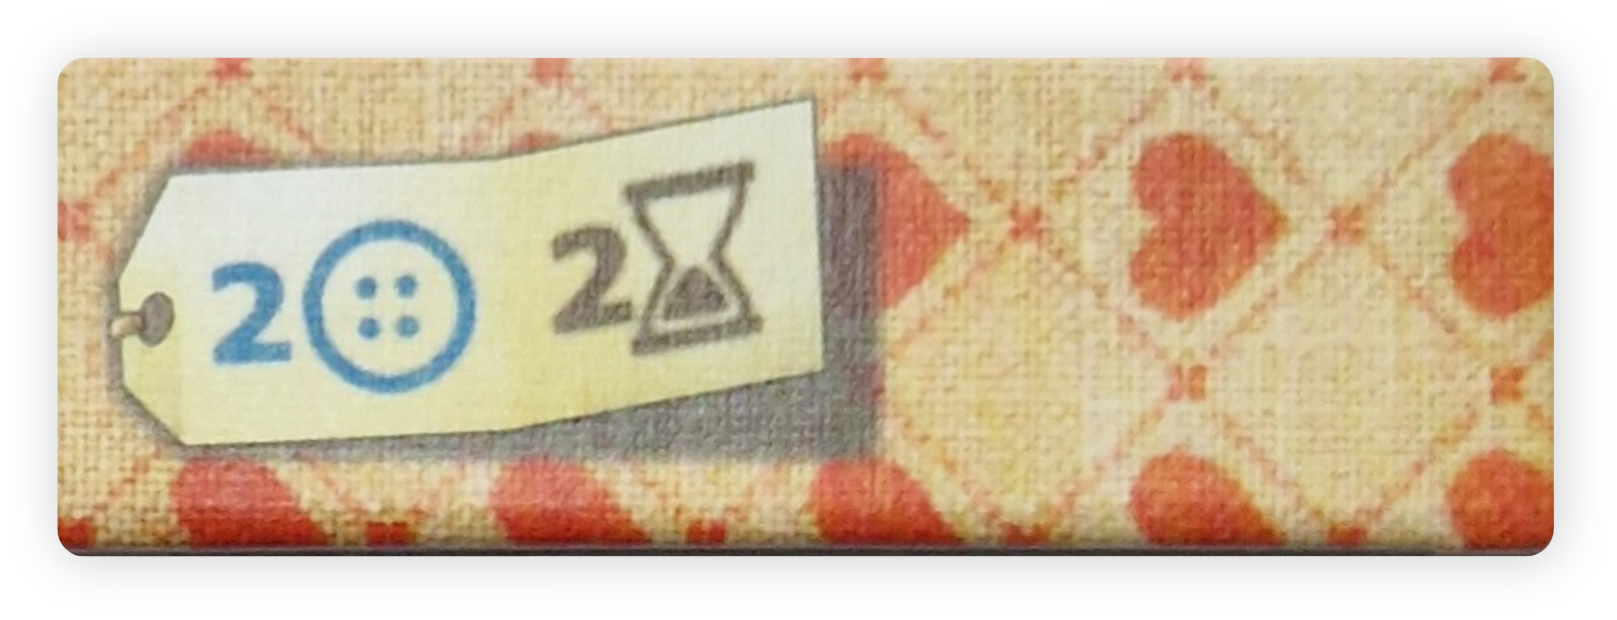
\includegraphics[width=0.2\textwidth]{res/pictures/assets/25-front.png}} & $25$ & $3$    & $2$              & $2$ & $0$ & $0$                            \\ \hline
    \adjustbox{valign=m, max width=0.2\textwidth, max height=0.1\textheight}{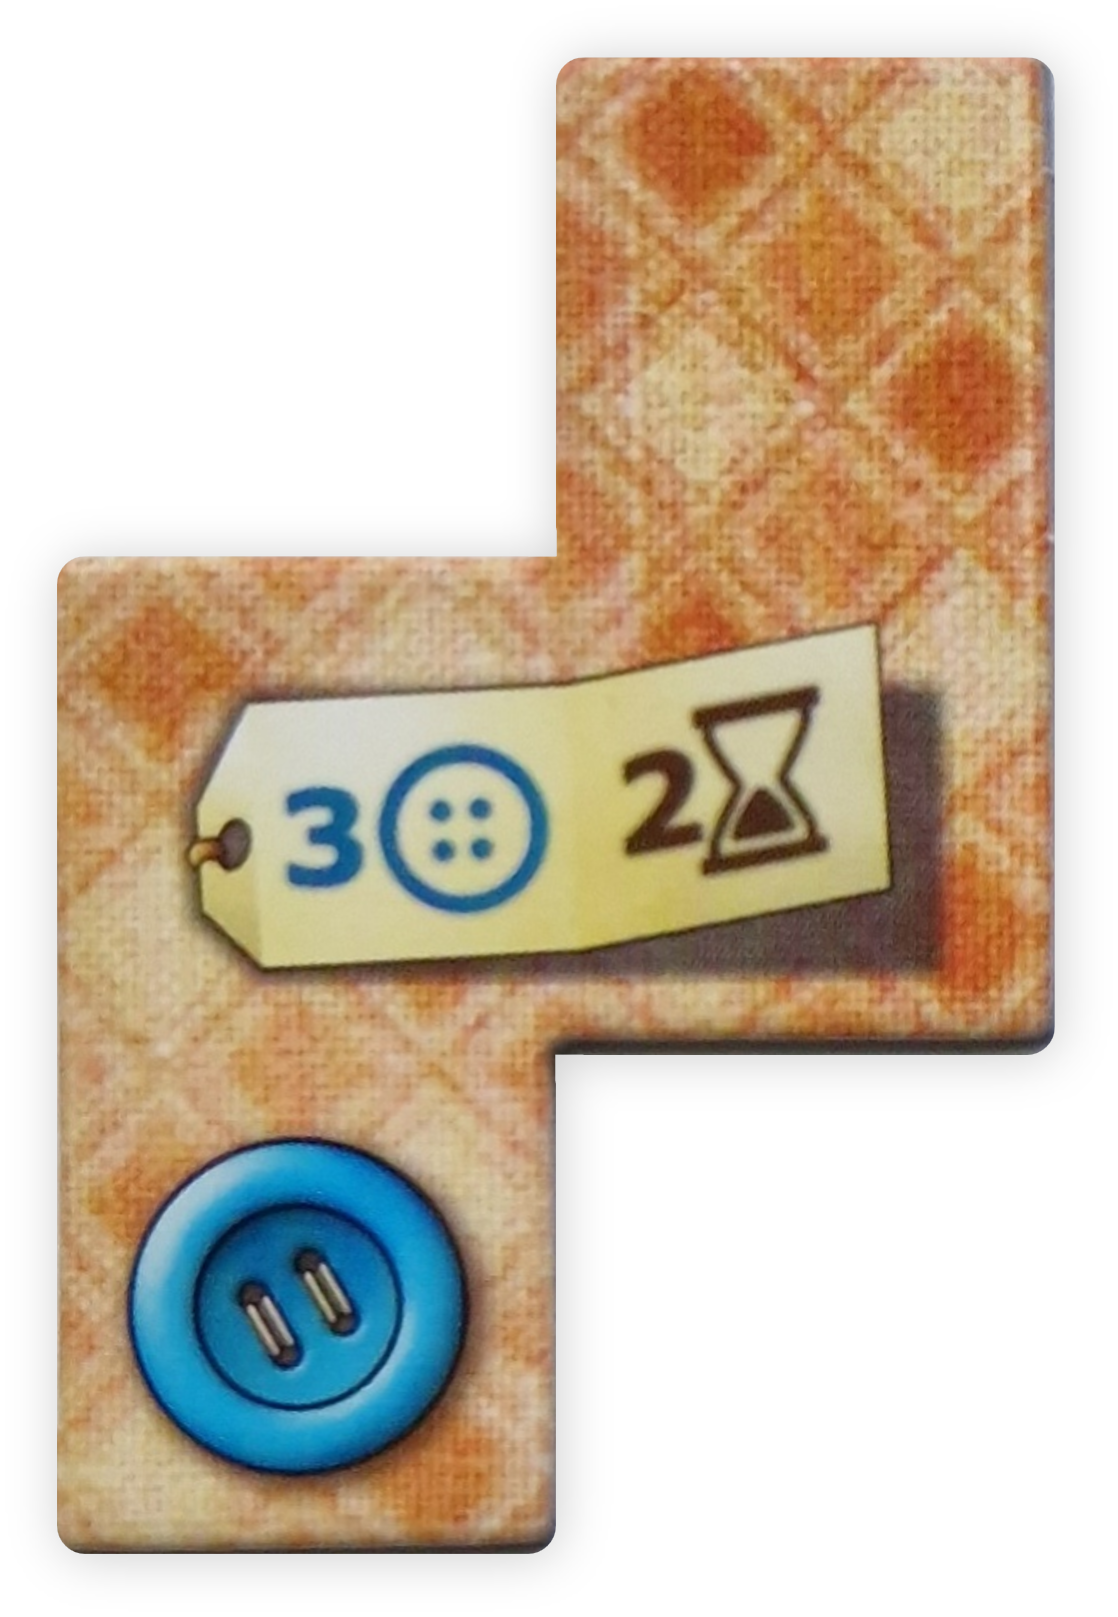
\includegraphics[width=0.2\textwidth]{res/pictures/assets/26-front.png}} & $26$ & $4$    & $3$              & $2$ & $1$ & $\frac{1}{8} = 0{,}125$        \\ \hline
    \adjustbox{valign=m, max width=0.2\textwidth, max height=0.1\textheight}{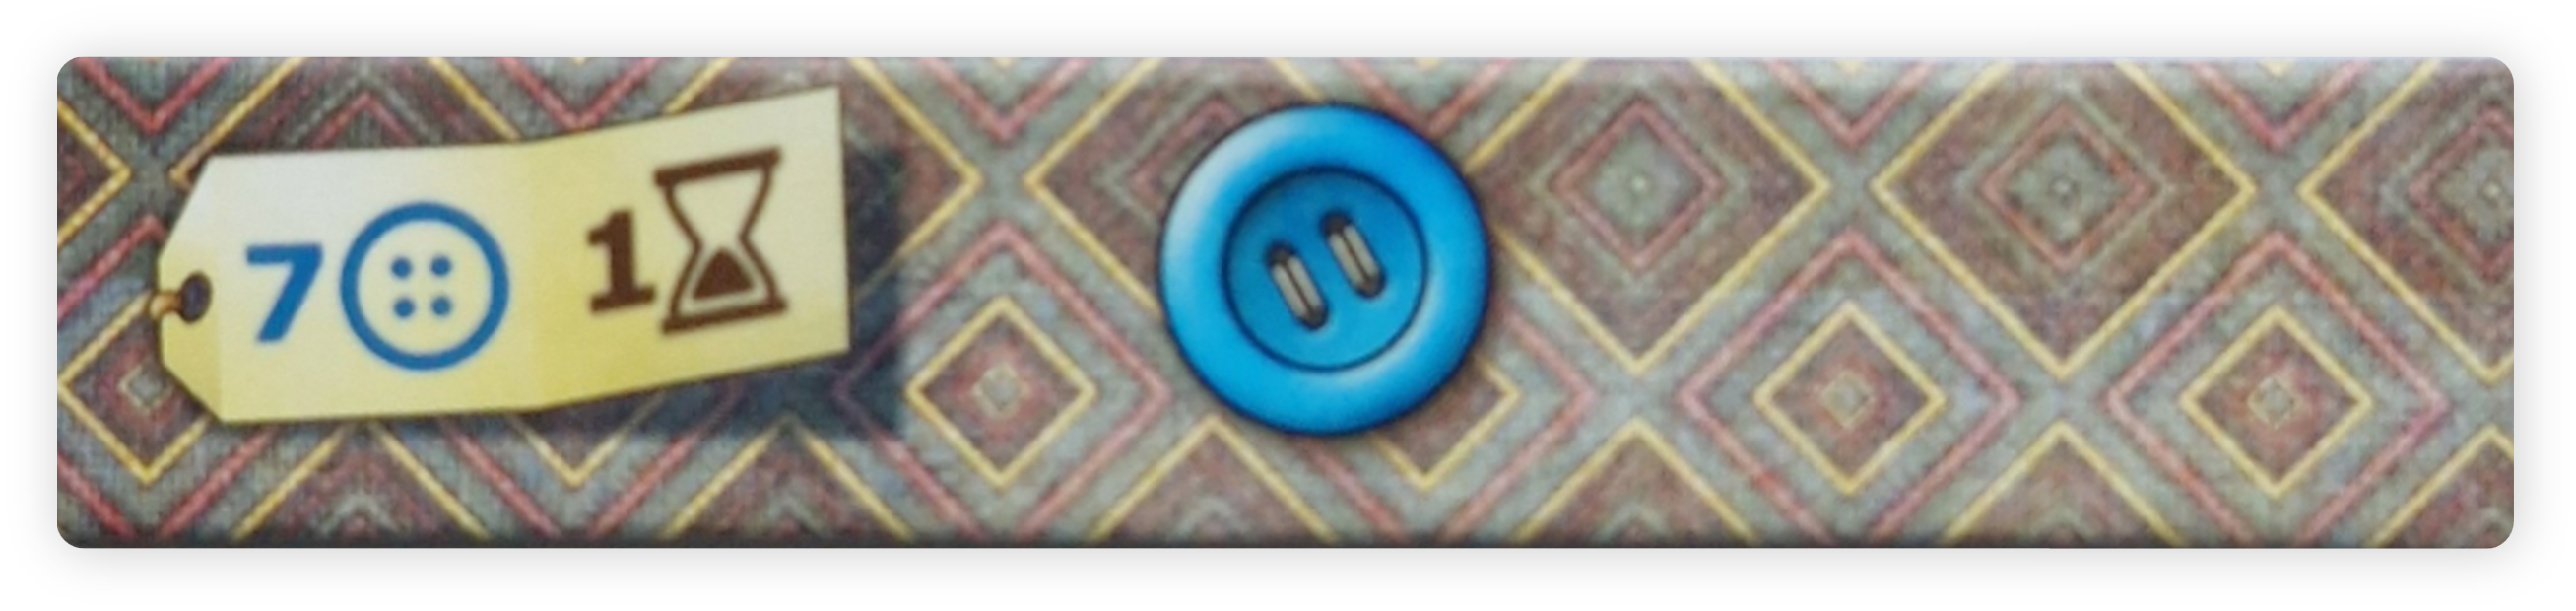
\includegraphics[width=0.2\textwidth]{res/pictures/assets/27-front.png}} & $27$ & $5$    & $7$              & $1$ & $1$ & $\frac{1}{5} = 0{,}2$          \\ \hline
    \adjustbox{valign=m, max width=0.2\textwidth, max height=0.1\textheight}{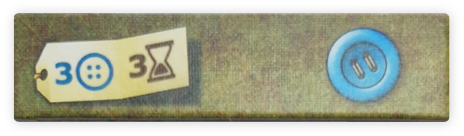
\includegraphics[width=0.2\textwidth]{res/pictures/assets/28-front.png}} & $28$ & $4$    & $3$              & $3$ & $1$ & $\frac{1}{12} \approx 0{,}083$ \\ \hline
    \adjustbox{valign=m, max width=0.2\textwidth, max height=0.1\textheight}{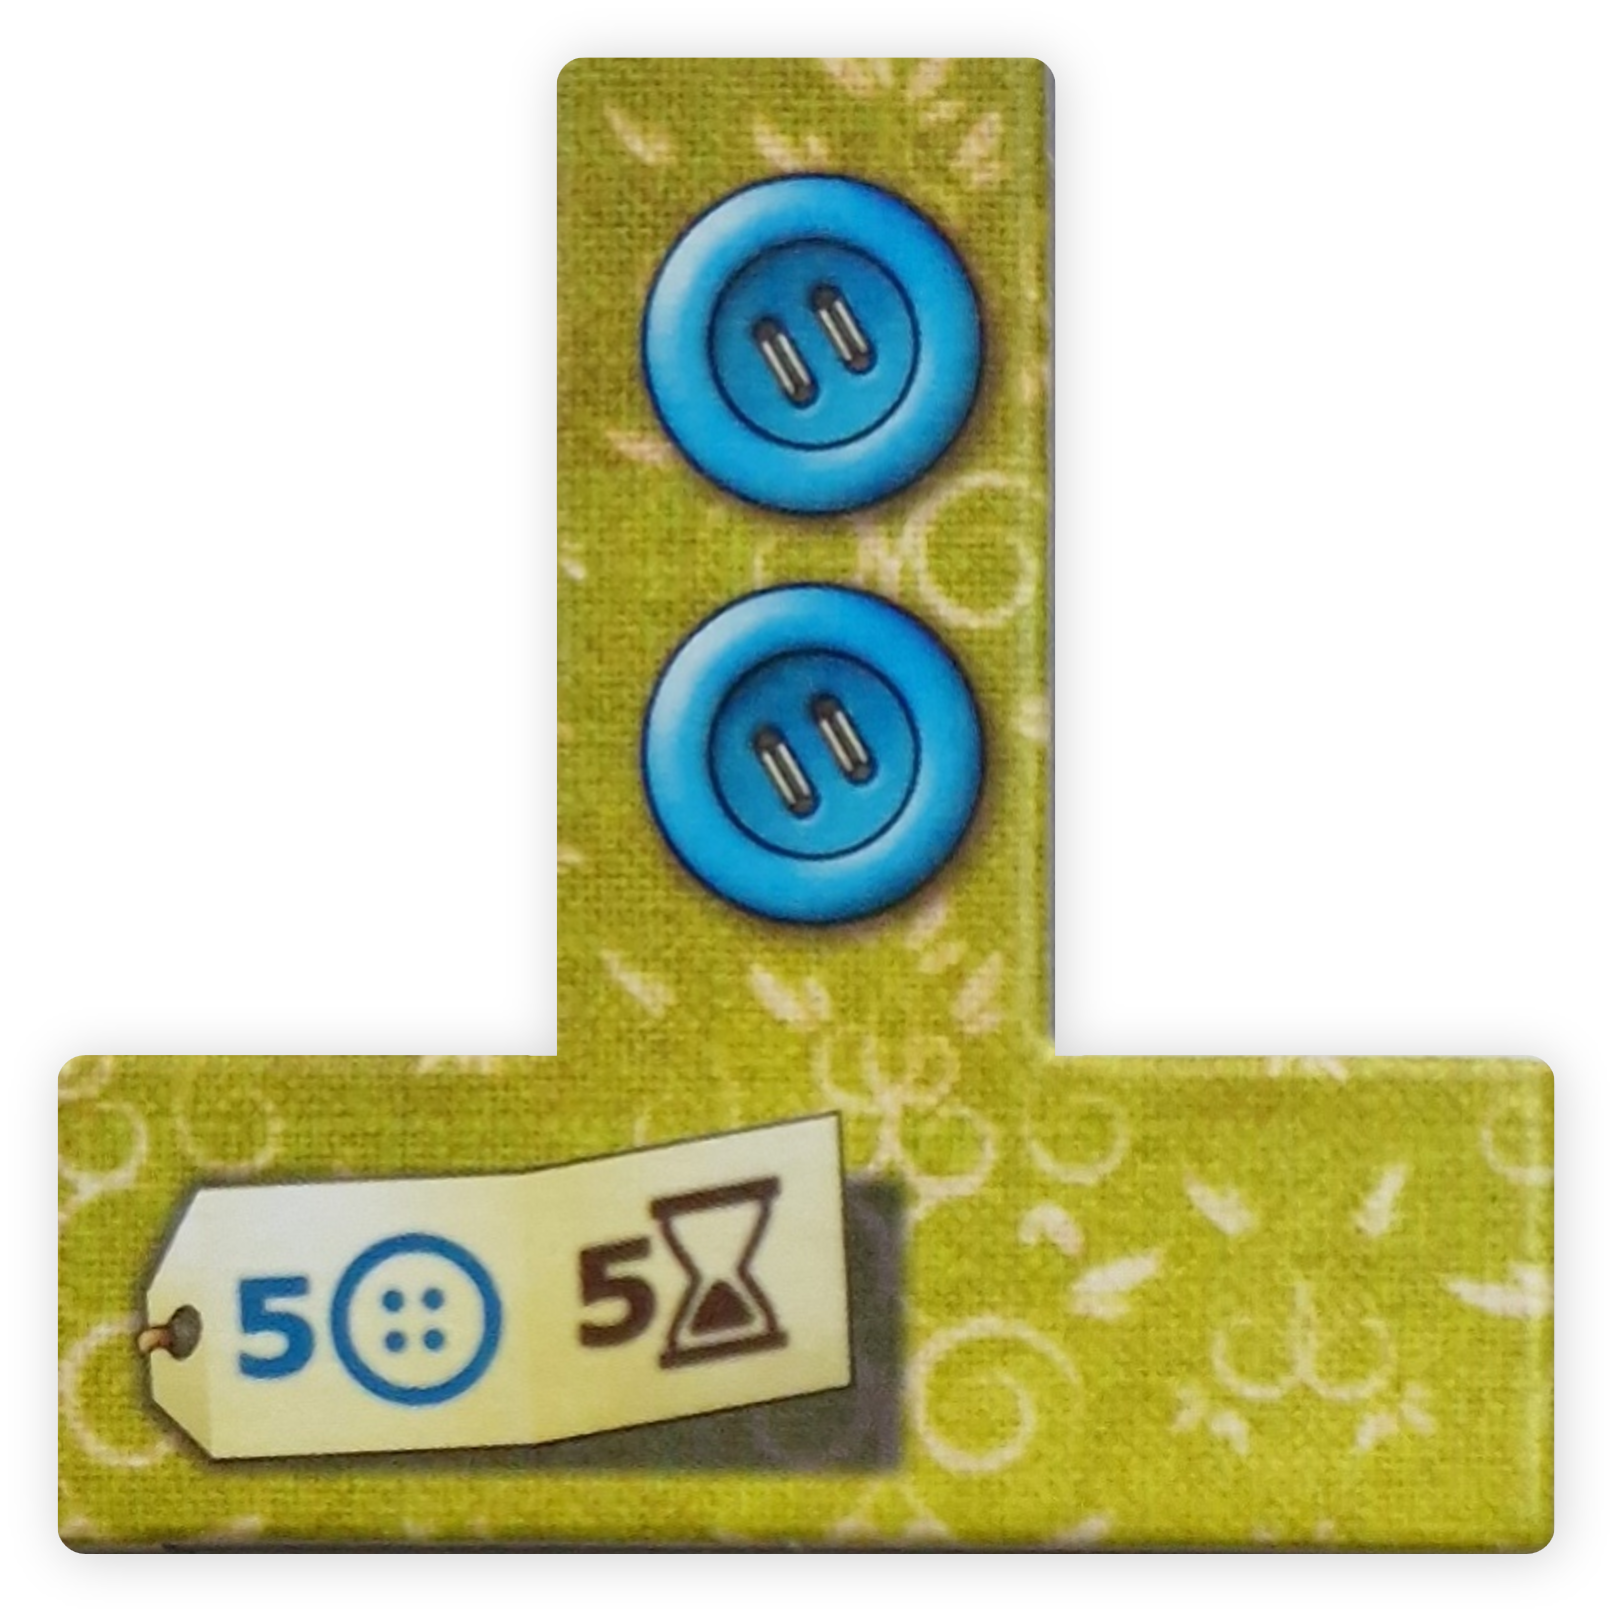
\includegraphics[width=0.2\textwidth]{res/pictures/assets/29-front.png}} & $29$ & $5$    & $5$              & $5$ & $2$ & $\frac{2}{25} = 0{,}08$        \\ \hline
    \adjustbox{valign=m, max width=0.2\textwidth, max height=0.1\textheight}{\includegraphics[width=0.2\textwidth]{res/pictures/assets/30-front.png}} & $30$ & $6$    & $3$              & $6$ & $2$ & $\frac{1}{18} \approx 0{,}056$ \\ \hline
    \adjustbox{valign=m, max width=0.2\textwidth, max height=0.1\textheight}{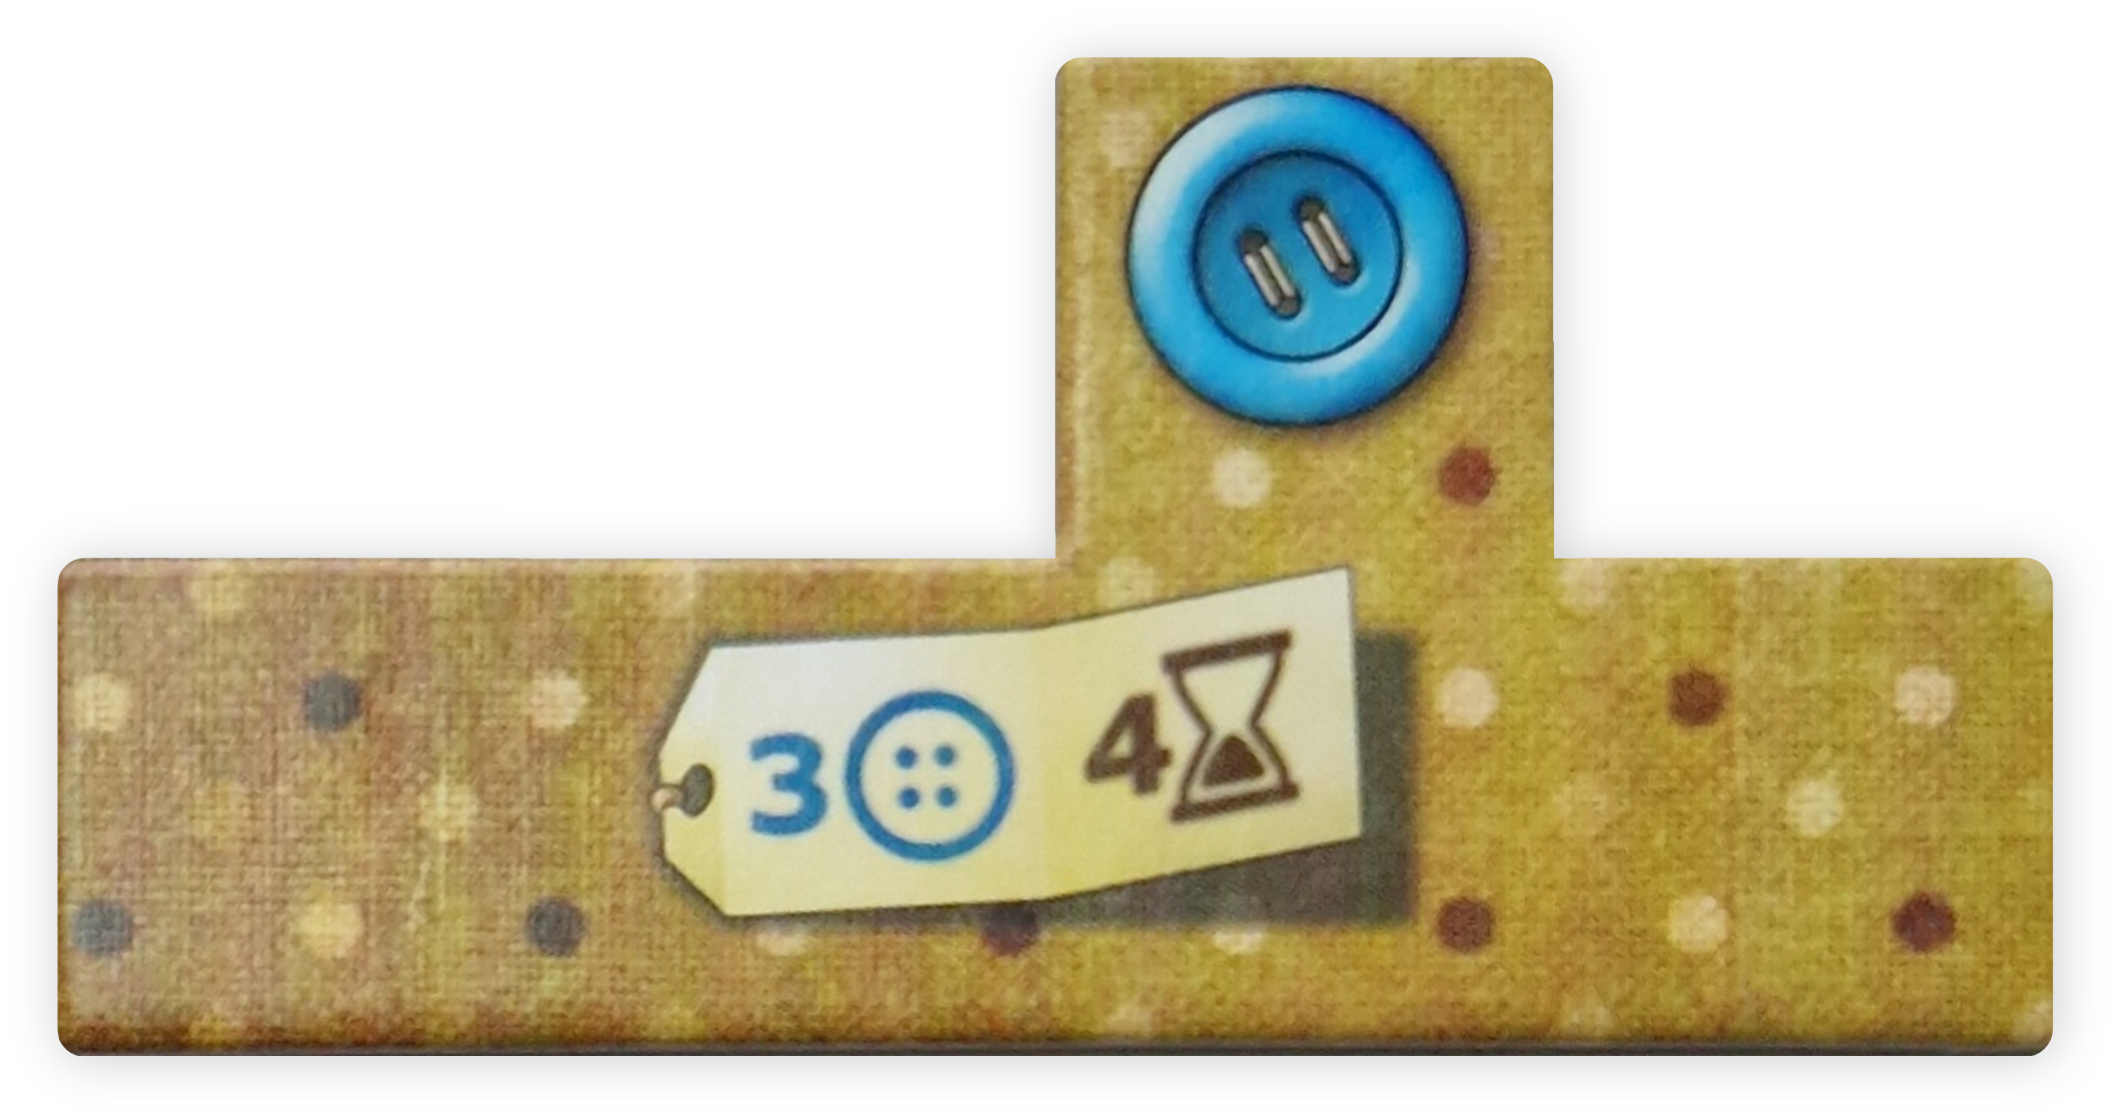
\includegraphics[width=0.2\textwidth]{res/pictures/assets/31-front.png}} & $31$ & $5$    & $3$              & $4$ & $1$ & $\frac{1}{20} = 0{,}05$        \\ \hline
    \adjustbox{valign=m, max width=0.2\textwidth, max height=0.1\textheight}{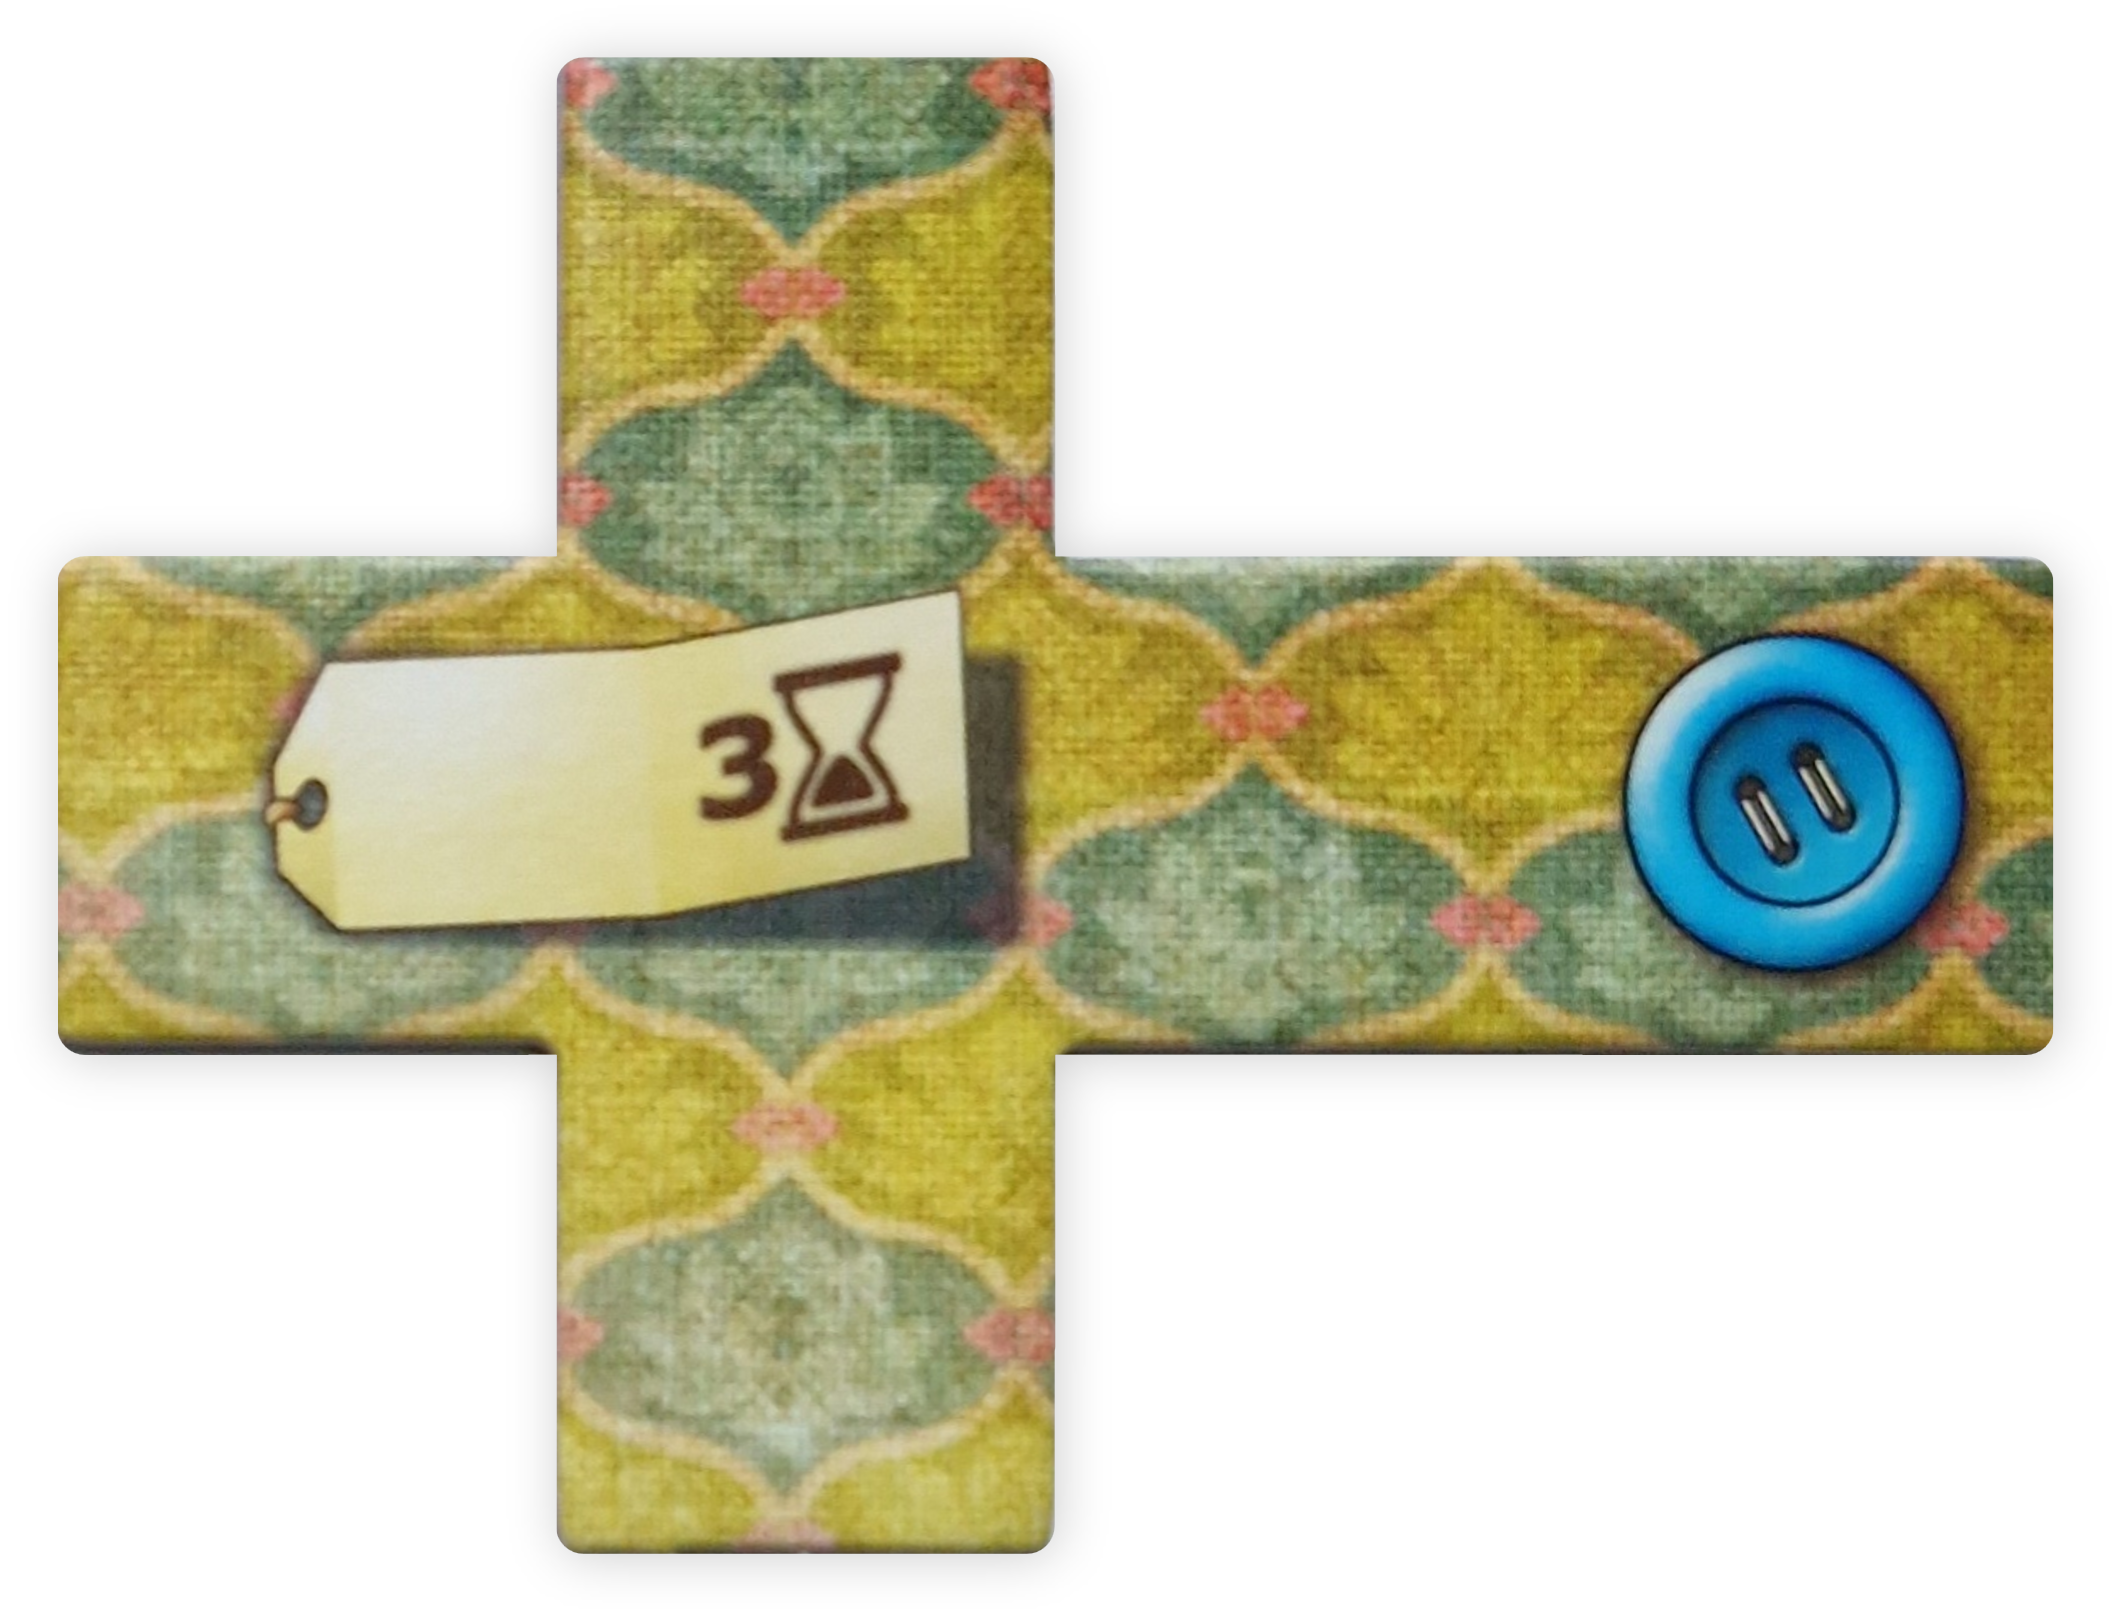
\includegraphics[width=0.2\textwidth]{res/pictures/assets/32-front.png}} & $32$ & $6$    & $0$              & $3$ & $1$ & $\frac{1}{18} \approx 0{,}056$ \\ \hline
\end{longtable}

% Reset to default
% \setlength{\tabcolsep}{6pt}

\newpage
\end{document}
